\documentclass[11pt, twoside, openright, a4paper, chapterprefix]{scrbook}
\usepackage[inner=2.5cm, outer=2.5cm, top=4cm, bottom=4cm]{geometry}

%%% PACKAGES %%%%%%%%%%%%%%%%%%%%%%%%%%%%%%%%%%%%%%%%%%%%%%%%%%%%%%%%%%%%%%%%%%
%%%%%%%%%%%%%%%%%%%%%%%%%%%%%%%%%%%%%%%%%%%%%%%%%%%%%%%%%%%%%%%%%%%%%%%%%%%%%%%
%%
%%          $Id: packages.tex 385 2013-02-12 21:53:10Z holz $
%%    author(s): RoboCupAtWork Technical Committee(s)
%%  description: List of packages for the RoboCupAtWork rulebook
%%
%%%%%%%%%%%%%%%%%%%%%%%%%%%%%%%%%%%%%%%%%%%%%%%%%%%%%%%%%%%%%%%%%%%%%%%%%%%%%%%
\usepackage{soul}

\usepackage[english]{babel}
\usepackage{amsmath,amssymb,amsfonts}
\usepackage[nice]{nicefrac}
\usepackage{siunitx}
\usepackage{graphicx}
\usepackage{multicol}
\usepackage{verbatim}
\usepackage{fancyhdr}
% \usepackage{svn-multi}
\usepackage{color}
\usepackage{xcolor,colortbl}
\usepackage{epsfig}
\usepackage{makeidx}
\usepackage{lscape}
\usepackage{picinpar}
% \usepackage{./styles/bar}
\usepackage{./styles/tweaklist}
%\usepackage{subfigure}
\usepackage{enumerate,paralist}
\usepackage{multirow}
\usepackage{pgffor}
\usepackage{array}
\usepackage{etoolbox}
\usepackage{hyperref}
\usepackage{tabularx}
\usepackage{xspace}

%\usepackage[utf8x]{inputenc}
%\usepackage{times}
%\usepackage{helvet}
%\usepackage{courier}

\usepackage{url}
\usepackage{caption}
%\usepackage{subcaption}
\usepackage{epstopdf}
\usepackage{subfig}
\usepackage{float}
\usepackage{wrapfig}
\usepackage{titlesec}
\usepackage{xfrac}

\usepackage[normalem]{ulem}  % used for \revadd, \revdel, etc.
\usepackage{xspace}  % used for adding spaces to macros, e.g. \RC, \RCAW, etc.
\usepackage[export]{adjustbox}  % used for valign option on images

% Local Variables:
% TeX-master: "../Rulebook"
% End:

\usepackage[titletoc]{appendix}
\usepackage{enumitem}
\usepackage{mathtools}
\usepackage{gensymb}
\usepackage[normalem]{ulem}
\setlist{noitemsep}
\usepackage{hhline}
\usepackage{rotating}
\usepackage{tikz}

\usetikzlibrary{arrows}
\usetikzlibrary{calc}
\usetikzlibrary{fit}
\usetikzlibrary{decorations.pathreplacing}
%%% SubfigureSetup %%%%%%%%%%%%%%%%%%%%%%%%%%%%%%%%%%%%%%%%%%%%%%%%%%%%%%%%%%%%
%\renewcommand{\subfigtopskip}{5pt}        % default is 10pt
%\renewcommand{\subfigbottomskip}{5pt}     % default is 10pt
%\renewcommand{\subfigcapskip}{3pt}        % default is 10pt
%\renewcommand{\subfigcapmargin}{7pt}      % default is 10pt

%%% TweakList-Setup %%%%%%%%%%%%%%%%%%%%%%%%%%%%%%%%%%%%%%%%%%%%%%%%%%%%%%%%%%%
\renewcommand{\itemhook}{%                 % modify itemize-spacing
  \setlength{\topsep}{2pt}%
  \setlength{\partopsep}{1pt}%
  \setlength{\itemsep}{-1pt}%
}
\renewcommand{\enumhook}{%                 % modify enumerate-spacing
  \setlength{\topsep}{2pt}%
  \setlength{\partopsep}{1pt}%
  \setlength{\itemsep}{-1pt}%
}
\renewcommand{\descripthook}{%             % modify description-spacing
  \setlength{\topsep}{2pt}%
  \setlength{\partopsep}{1pt}%
  \setlength{\itemsep}{-1pt}%
}

\setkomafont{title}{\normalfont}
\setkomafont{sectioning}{\normalfont\bfseries}
\addtokomafont{caption}{\small}
\setkomafont{captionlabel}{\small\bfseries}
\setkomafont{descriptionlabel}{\normalfont\bfseries}
\renewcommand*{\chapterformat}{\LARGE{Chapter \thechapter}}

\setcounter{secnumdepth}{3}

\setlength{\parskip}{10pt plus 1pt minus 1pt}
\setlength{\parindent}{0pt}

%%% MACROS %%%%%%%%%%%%%%%%%%%%%%%%%%%%%%%%%%%%%%%%%%%%%%%%%%%%%%%%%%%%%%%%%%%%
\newcommand{\YEAR}{2018\xspace}
\newcommand{\STATE}{Preliminary}

%%%%%%%%%%%%%%%%%%%%%%%%%%%%%%%%%%%%%%%%%%%%%%%%%%%%%%%%%%%%%%%%%%%%%%%%%%%%%%%
%%
%%          $Id: macros.tex 399 2013-02-14 20:24:02Z holz $
%%    author(s): RoboCupAtHome Technical Committee(s)
%%  description: Macros for the RoboCupAtWork rulebook
%%
%%%%%%%%%%%%%%%%%%%%%%%%%%%%%%%%%%%%%%%%%%%%%%%%%%%%%%%%%%%%%%%%%%%%%%%%%%%%%%%

%%%%%%%%%%%%%%%%%%%%%%%%%%%%%%%%%%%%%%%%%%%%%%%%%%%%%%%%%%%%%%%%%%%% 
% Macros for generating score sheets for RoboCup@Work              %
% to be used in the rulebook or during the competition             %
%                                                                  % 
% Author: Dirk Holz & David Gossow                                 %
% Modif : Mauricio Matamoros                                       %
% $Id: macros_score_sheets.tex 429 2013-04-30 10:09:55Z holz $     %
%%%%%%%%%%%%%%%%%%%%%%%%%%%%%%%%%%%%%%%%%%%%%%%%%%%%%%%%%%%%%%%%%%%% 


\usepackage{calc}
\usepackage{ifthen}
\usepackage{wasysym}
\usepackage{chngpage}


%%% Counters / temp. variables %%%%%%%%%%%%%%%%%

\newcounter{currTestScore}
\newcounter{currTestScoreTotal}
\newcounter{currTestScoreTotalWithoutBonus}
\newcounter{currOutstandingBonus}
\newcommand{\scorelistOptions}{}
\newcommand{\scoresheetOptions}{}

% set \shortScoresheet to true for the rulebook version and to false for the referee's scoresheet
\newcommand{\shortScoresheet}{true}

% set \threeAttempts to true for three columns in the scoresheet
\newcommand{\threeAttempts}{false}

% set \retryAvailable to true for a second column in the scoresheet
\newcommand{\retryAvailable}{true}

% set \continueAvailable to true for CONTINUE sections
\newcommand{\continueAvailable}{true}

% name of the current test, is set automatically in the rulebook
\newcommand{\currentTest}{}

% (internal) if-clause shortcut to switch between short rulebook version and full score sheet for referees
\newcommand{\ifShortScoresheet}[2]{%
  \ifthenelse{ \equal{\shortScoresheet}{true}}{%
    #1%
  }{%
    #2%
  }%
}

\newcommand{\ifEvaluationSheet}[2]{%
  \ifthenelse{ \equal{\scoresheetOptions}{evaluationSheet}}{%
    #1%
  }{%
    #2%
  }%
}

% (internal) draws the scoresheet line for score handwritting
\newcommand{\scoreline}[1][0.08]{\rule{#1\linewidth}{.2pt}}

% (internal) draws the lines for score hadndwritting in the table outline based on the number of attempts
\newcommand{\attemptScoreLines}{
  \switchAttempts
    {\scoreline[0.06] & \scoreline[0.06] & \scoreline[0.06]}
    {\scoreline & \scoreline}
    {\scoreline}
}

% (internal) Select one of the provided arguments based on the number of attempts
% (3 tries, retry (2) or only try (1))
\newcommand{\switchAttempts}[3]{
  \ifthenelse{\equal{\threeAttempts}{true}}{#1}{\ifthenelse{\equal{\retryAvailable}{true}}{#2}{#3}}
}

% (internal) stores the number of attempts to perform
\edef\numAttempts{0}
% (internal) writes on the command \numAttempts the number of attempts to perform
\newcommand\defNumAttempts{
  \switchAttempts
  {\global\edef\numAttempts{3}}
  {\global\edef\numAttempts{2}}
  {\global\edef\numAttempts{1}}
}

%% commands for overriding internal calculations %%%%%%%%%%%%%%%%%%%%%%%%%%%%%%%%%%%%%%%%

% set score counter to arbitrary value
\newcommand{\setTotalScore}[1]%
{%
  \setcounter{currTestScore}{#1}
}

% set outstanding bonus to arbitrary value
\newcommand{\setOutstandingBonus}[1]%
{%
  \setcounter{currOutstandingBonus}{#1}
}




%% Score sheet page layout %%%%%%%%%%%%%%%%%%%%%%%%%%%%%%%%%%%%%%%%%%%%%%%%%%%%%%%%%%%%%%%%

% usage: \begin{scoresheet}[repeatable] ... \end{scoresheet}
\newenvironment{scoresheet}[1][]{
  % begin
  \newpage

  \renewcommand{\scoresheetOptions}{#1}
  
  \begin{minipage}[t]{0.8\textwidth}%
    \vspace{0pt}
    {\huge \textbf{Score Sheet} }
    
    \vspace{2 em}
    
    \begin{tabular}{ @{} l l l}
      \textbf{Test:} & \currentTest \\[.9 em]
      
      \ifEvaluationSheet{}{%
        \textbf{Team name:} & \scoreline[0.6]\\[.9 em]%
      }%
      % 
      \textbf{Referee name:} & \scoreline[0.6]\\[.9 em]%
      %	
      %	\ifEvaluationSheet{}{%
      %   \textbf{Restart:} & \Square ~1st try \hspace{1 em} \Square ~2nd try
      %	}
      %	
      % test repetition checkboxes (for stage 2 tests)
      \ifthenelse{ \equal{#1}{repeatable} }{%
	\textbf{Test repetition:} & \Square ~1st \hspace{1 em} \Square ~2nd\\[.9em]%
      }{}
    \end{tabular}

    \vspace{0.5 em}

  \end{minipage}
  \hfill
  \begin{minipage}[t]{0.15\textwidth}%
    \vspace{0pt}
    \includegraphics[width=\textwidth]{images/logo_RoboCupAtHome.jpg}%
  \end{minipage}\\
}
{
  % end
  \vspace{.2 em}
  \textbf{Remarks:}

  %% signatures of referee / team leader %%%%%%%%%%%%
  \vfill
  \ifEvaluationSheet{
    % team evaluation sheet
    \begin{tabular}{@{} @{\extracolsep{\fill}} l l @{}}
      \scoreline[0.25] \hspace{0.05\linewidth} & \scoreline[0.25] \hspace{0.05\linewidth}
      \\
      \textit{Date \& time}%
      & \textit{Referee}
    \end{tabular}
  }{
    % normal sheet
    \begin{tabular}{@{} @{\extracolsep{\fill}} l l l @{}}
      \scoreline[0.25] \hspace{0.05\linewidth} & \scoreline[0.25] \hspace{0.05\linewidth} & \scoreline[0.25]
      \\
      \textit{Date \& time}%
      & \textit{Referee} %
      & \textit{Team leader}
    \end{tabular}
  }

  \newpage
}


%% Score list table %%%%%%%%%%%%%%%%%%%%%%%%%%%%%%%%%%%%%%%%%%%%%%%%%%%%%%%%%%%%%%%%

% usage: \begin{scorelist}[openDoorSignal] ... \end{scorelist}
\newenvironment{scorelist}[1][]{
  % begin

  % init variables %%%%%%%%%
  \renewcommand{\scorelistOptions}{#1}
  \setcounter{currTestScore}{0}
  \setcounter{currOutstandingBonus}{0}

  % setup table %%%%%%%%%
  \vspace{0.8 em}

  \ifShortScoresheet {
    \begin{tabular*}{\textwidth}{@{} @{\extracolsep{\fill}} p{0.8\linewidth} r @{}}
      \ifEvaluationSheet{
        \textbf{Team} & \textbf{Score} \\ \hline 
      }{%
        \textbf{Action} & \textbf{Score} \\ \hline 
      }
    }{  
      % else:
      % \begin{tabular*}{\textwidth}{@{}p{0.65\linewidth}lp{0.15\linewidth}@{}}
      %   \textbf{Action} & \textbf{Score} & \multicolumn{1}{l}{\textbf{Success}}\\ \hline 
      \ifEvaluationSheet{
        \begin{tabular*}{\textwidth}{@{} @{\extracolsep{\fill}} p{0.7\linewidth} r r @{}}
          \textbf{Team} & \textbf{Score} & \textbf{Result}\\ \hline 
        }{
          \ifthenelse{\equal{\threeAttempts}{true}}{
            \begin{tabular*}{\textwidth}{@{} @{\extracolsep{\fill}} p{0.6\linewidth} r r r r @{}}
            \textbf{Action} & \textbf{Score} & \textbf{\small $1^{st}$ try} & \textbf{\small $2^{nd}$ try} & \textbf{\small$3^{rd}$ try} \\ \hline 
          }
          %else
          {
            \begin{tabular*}{\textwidth}{@{} @{\extracolsep{\fill}} p{0.6\linewidth} r r r @{}}
            \textbf{Action} & \textbf{Score} \ifthenelse{\equal{\retryAvailable}{true}}{& \textbf{1st try} & \textbf{2nd try}}{ & \textbf{Only try}} \\ \hline 
          }
        }
      }
    }
      {
        % end

	\ifEvaluationSheet{}{%
          
          % calculate max. score, outstanding bonus %%%%%%%
          \ifthenelse{\value{currOutstandingBonus} = 0}{%
            \setcounter{currOutstandingBonus}{ \value{currTestScore} / 10 }
          }{}
          \setcounter{currTestScoreTotal}{ \value{currTestScore} + \value{currOutstandingBonus} }
          \setcounter{currTestScoreTotalWithoutBonus}{ \value{currTestScore} }
          

          % Special penalties & bonuses %%%%%%%%%%%%%%%%
          \scoreheading{Special penalties \& bonuses}
          \ifShortScoresheet{}{
          	\ifthenelse {\equal{\continueAvailable}{true}}{\scoreitem[0.75]{0}{1st CONTINUE}}{}
          
          	\ifthenelse {\equal{\continueAvailable}{true}}{\scoreitem[0.50]{0}{2nd CONTINUE}}{}
		  }
          
          \scoreitem{-50}{Not attending \ifShortScoresheet{(see sec.~\ref{rule:not_attending})}{}}
          
          \ifthenelse{\equal{\scorelistOptions}{openDoorSignal}}{
            \scoreitem{-10}{Using start button \ifShortScoresheet{(see sec.~\ref{rule:start_button})}{}}
          }{}

          % \ifthenelse{\value{currOutstandingBonus} = 0}{
          \scoreitem{\thecurrOutstandingBonus}{Outstanding performance \ifShortScoresheet{(see sec.~\ref{rule:outstanding_performance})}{}}
          % }{}
          
          % Total score %%%%%%%%%%%%%%%%
          \hline\\
          % \textbf{Total score} & \scoring{ \thecurrTestScoreTotal } %
          \ifShortScoresheet {%
            % No Score per try in short version
          }{%
            \textbf{\textit{Score per try}} & \scoring{ \thecurrTestScoreTotalWithoutBonus } %
          }
          % add line to put in total:
          \ifShortScoresheet{}{& \attemptScoreLines} \\   
          \ifShortScoresheet{
            \textbf{Total score} (excluding penalties and bonuses) & \scoring{ \thecurrTestScoreTotalWithoutBonus } %
          }{
            \defNumAttempts
            & \\
            \textbf{Total score}  & \scoring{ \thecurrTestScoreTotalWithoutBonus } & \multicolumn{\numAttempts}{c}{\scoreline[0.20]}
          } \\
	}

      \end{tabular*}
      
    }


    %% Score sheet table entries %%%%%%%%%%%%%%%%%%%%%%%%%%%%%%%%%%%%%%%%%%%%%%%%%%%%%%%%%%%%%%%%

    % for loop helper
    % usage: \forloop[step]{counter}{initial_value}{conditional}{code_block} 
    \newcommand{\forloop}[5][1]%
    {%
      \setcounter{#2}{#3}%
      \ifthenelse{#4}%
      {%
 	#5%
 	\addtocounter{#2}{#1}%
 	\forloop[#1]{#2}{\value{#2}}{#4}{#5}%
      }%
      % else
      {%
      }%
    }

    \newcounter{ct}

    % heading
    % usage: \scoreheading{text}
    \newcommand{\scoreheading}[1]{
      \ifShortScoresheet {%
        \phantom{.} \\[-4 ex] \multicolumn{2}{@{}l}{\textbf{\textit{#1}}}\\[0pt]
      }{%
        \phantom{.} \\[-4 ex] \multicolumn{3}{@{}l}{\textbf{\textit{#1}}}\\[0pt]
      }
    }

    % table entry
    % usage: \scoreitem[multiplicity]{points}{description}
    \newcommand{\scoreitem}[3][1]{

      % add to max. total score if points > 0
      \ifthenelse{ #2 > 0 }{
        \addtocounter{currTestScore}{ #2 * #1 }
      }{}%
      % 
      \begin{minipage}[t]{\linewidth} {#3} \vspace{0.1 em} \end{minipage} & %
      \scoring{ \ifthenelse{ \equal{#1}{1} }{}{ #1 $\times$} \ifthenelse{ \equal{#2}{0} }{}{ #2}}%
      % insert check marks:	
      %	\ifShortScoresheet{}{ & \forloop{ct}{0}{\value{ct} < #1}{ \Square}} \\[3pt]
      % insert line
      \ifShortScoresheet{ %
        \\ 
      }{ % else
        \ifEvaluationSheet{}{& \attemptScoreLines} \\[0pt]
      }
    }


% Local Variables:
% TeX-master: "../Rulebook"
% End:

%%%%%%%%%%%%%%%%%%%%%%%%%%%%%%%%%%%%%%%%%%%%%%%%%%%%%%%%%%%%%%%%%%%%%%%%%%%%%%%
%%
%%          $Id: macros_open_demonstrations.tex 391 2013-02-14 07:57:07Z sugiura $
%%    author(s): holz
%%  description: simple macros for specifications of open challenges
%%
%%%%%%%%%%%%%%%%%%%%%%%%%%%%%%%%%%%%%%%%%%%%%%%%%%%%%%%%%%%%%%%%%%%%%%%%%%%%%%%

\newcommand{\OpenDemonstrationTask}[2] {
  \begin{enumerate}%
    \item \textbf{Setup and demonstration:} The team has a maximum of \timing{#1 minutes} for setup, presentation and demonstration.%
    \item \textbf{Interview and cleanup:} After the demonstration, there is
	      another \timing{#2 minutes} where the team answers %
    questions by the jury members.\\%
    During the interview time, the team has to undo its changes to the environment.%
  \end{enumerate}%
}

\newcommand{\OpenDemonstrationChanges}{
  \subsection{Changes to the environment}
  \begin{enumerate}
    \item \textbf{Making changes:} As in the other open demonstrations, teams are allowed to make modifications to the arena as they like, 
    but under the condition that they are reversible.
    \item \textbf{Undoing changes:} In the interview and cleanup team, changes need to be made undone by the team. 
    The team has to leave the arena in the \emph{very same} condition they entered it.
  \end{enumerate}
}
% Local Variables:
% TeX-master: "../Rulebook"
% End:


\newcommand{\rulebookVersion}{\STATE\ version for RoboCup \YEAR}

\def\RC{RoboCup\xspace}
\def\RCAW{RoboCup@Work\xspace}

\renewcommand{\labelenumi}{\arabic{enumi}.}
\renewcommand{\labelenumii}{\labelenumi\arabic{enumii}.}
\renewcommand{\labelenumiii}{\labelenumii.\arabic{enumiii}.}


%% %%%%%%%%%%%%%%%%%%%%%%%%%%%%%%%%%%%%%%%%%%%%%%%%%%%%%%%%% %%
%%                    Developement-Tools                     %%
%% %%%%%%%%%%%%%%%%%%%%%%%%%%%%%%%%%%%%%%%%%%%%%%%%%%%%%%%%% %%

%% %%%%%%%%%%%%%%%%%%%%%%%%%%%%%%%%%%%%%%%
\newcommand{\tbc}[1]{\textbf{\it\color{red}{t.b.c. ...}#1\color{black}}}
\newcommand{\todo}[1]{\textbf{\it\color{red}{todo: }#1\color{black}}}
\newcommand{\TODO}[1]{\textbf{\it\color{red}{TODO:\\}#1\color{black}}}
\newcommand{\chk}[1]{\textbf{\color{red}#1\color{black}}}

\newcommand{\revadd}[1]{\textcolor{blue}{#1}}
\newcommand{\revdel}[1]{\textcolor{red}{\sout{#1}}}
\newcommand{\revcha}[2]{\revdel{#1}\revadd{#2}}

\newcommand{\reworkon}{\marginpar{\raggedright\color{red}{$\downarrow$rework}\color{black}}}
\newcommand{\reworkoff}{\marginpar{\raggedright\color{red}{$\uparrow$rework}\color{black}}}

%% %%%%%%%%%%%%%%%%%%%%%%%%%%%%%%%%%%%%%%%
%%  site notes/margin notes
\def\note#1{\marginpar{\raggedright\tiny\color{blue}#1}}
\def\mpar#1{\marginpar{\raggedright\tiny#1}}
\def\rand#1{\marginpar{\raggedright\tiny#1}}
\setlength{\marginparwidth}{2cm}

\newcommand{\refsec}[1]{Section~\ref{#1}}
\newcommand{\reftab}[1]{Table~\ref{#1}}
\newcommand{\reffig}[1]{Figure~\ref{#1}}

%% %%%%%%%%%%%%%%%%%%%%%%%%%%%%%%%%%%%%%%%
%% side-annotation-macros for easy lookup
% \newcommand{\awardmark}{\marginpar{\centering\includegraphics[width=.34cm]{images/icon_award.pdf}}}
% \newcommand{\refmark}{\marginpar{\centering\includegraphics[width=.5cm]{images/icon_whistle.pdf}}}
% \newcommand{\referee}[1]{\emph{#1}\marginpar{\centering\includegraphics[width=.5cm]{images/icon_whistle.pdf}}}
% \newcommand{\scoremark}{\marginpar{\centering\includegraphics[width=.34cm]{images/icon_score.pdf}}}
\newcommand{\awardmark}{}
\newcommand{\refmark}{}
\newcommand{\referee}[1]{}
\newcommand{\scoremark}{}
%\newcommand{\scoring}[1]{\emph{#1}\marginpar{\centering\includegraphics[width=.34cm]{images/icon_score.pdf}}}
\newcommand{\scoring}[1]{\emph{#1}}
\newcommand{\timark}{\marginpar{\centering\includegraphics[width=.34cm]{icon_clock.pdf}}}

%\newcommand{\timing}[1]{\emph{#1}\marginpar{\centering\includegraphics[width=.34cm]{images/icon_clock.pdf}}}
\newcommand{\timing}[1]{\emph{#1}}

\def\svnRevision{Unknown} %
\def\svnChangeData{Unknown} %
\def\revnumtmpfile{.temp_rulebook_version}
\def\revdattmpfile{.temp_rulebook_date}
\immediate\write18{git rev-list HEAD | wc -l > \revnumtmpfile}
%\immediate\write18{svnversion . > \revnumtmpfile}
\IfFileExists{\revnumtmpfile}{\def\svnRevision{\input{\revnumtmpfile}\unskip}}{} 
\immediate\write18{git log -1 --date=short  | grep 'Date:' | awk '{print $2}'> \revdattmpfile}
%\immediate\write18{svn info | grep 'Last Changed Date:' | awk '{print $4}'> \revdattmpfile}
\IfFileExists{\revdattmpfile}{\def\svnChangeData{\input{\revdattmpfile}\unskip}}{} 
% \IfFileExists{\revnumtmpfile}{\immediate\write18{rm -f \revnumtmpfile}}{} 
% \IfFileExists{\revdattmpfile}{\immediate\write18{rm -f \revdattmpfile}}{} 
\newcommand{\VERSION}{Revision \svnChangeData\_\svnRevision}


% Local Variables:
% TeX-master: "../Rulebook"
% End:

%% %%%%%%%%%%%%%%%%%%%%%%%%%%%%%%%%%%%%%%%%%%%%%%%%%%%%%%%%%%%%%%%%%%%%%%%%%%%
%%
%%          $Id: abbrevix.tex 373 2013-02-12 20:32:49Z holz $
%%    author(s): RoboCupAtHome Technical Committee(s)
%%  description: Abbreviations for the RoboCupAtHome RuleBook
%%
%% %%%%%%%%%%%%%%%%%%%%%%%%%%%%%%%%%%%%%%%%%%%%%%%%%%%%%%%%%%%%%%%%%%%%%%%%%%%

%% temp-variables %%%%%%%%%
\newlength{\adxtemp}
\newlength{\adxspace}
\setlength{\adxspace}{3cm}

%% %%%%%%%%%%%%%%%%%%%%%%%%%%%%%%%%%%%%%%%
%%  Commands to use this
%% %%%%%%%%%%%%%%%%%%%%%%%%%%%%%%%%%%%%%%%

%% \abb{abk}
%% to reference an abbreviation
\newcommand{\abb}[1]{\hypertarget{#1}{#1}}

%% \term{the term}
%% print 'the term' in italic,
%% do not include 'the term' in index
%\newcommand{\term}[1]{#1\index{#1}}
\newcommand{\term}[1]{\textit{#1}}

%% \iterm{the term}
%% print 'the term' in italic,
%% include 'the term' in index
\newcommand{\iterm}[1]{\textit{#1}\index{#1}}

%% \nterm{the term}
%% do NOT print 'the term' but include 'the term' in index
\newcommand{\nterm}[1]{\index{#1}}

%% \TERM
%% print first term, add second term to index
\newcommand{\Term}[2]{\textit{#1}\index{#2}}


%% \aterm{the term}{abb}
%% print 'term', 
%% include 'term' with abbreviation 'abb' in abbreviation-index
\newcommand{\aterm}[2]{\settowidth{\adxtemp}{#2}{\hypertarget{#2}{#1 (#2)}\abbex{#2\hspace{\adxspace}\hspace{-\the\adxtemp}#1}}}

%% \iaterm{the term}{abbreviation} 
%% print 'term', 
%% include 'the term' in index, 
%% and include abbreviation in abbreviation-index
\newcommand{\iaterm}[2]{\settowidth{\adxtemp}{#2}{\hypertarget{#1}{\textit{#1} (#2)}\index{#1}\abbex{#2\hspace{\adxspace}\hspace{-\the\adxtemp}#1}}}

%% %%%%%%%%%%%%%%%%%%%%%%%%%%%%%%%%%%%%%%%
%%  Main Abbreviation Definitions
%% %%%%%%%%%%%%%%%%%%%%%%%%%%%%%%%%%%%%%%%

\makeatletter
\newlength{\QZ@TOChdent}% Used to define hanging indents.
\setlength{\QZ@TOChdent}{1.0em}%
\renewcommand{\@pnumwidth}{1.55em}%
\makeatother
%
%\newenvironment{simpleenv}[4]{\clearpage}{\clearpage}%
%\newenvironment{simpleenv}[4]{\clearpage}{\pagebreak}%
\newenvironment{simpleenv}[4]{\pagebreak}{\pagebreak}%
\newcommand{\BaseDiff}{0}%
%\newcommand{\RSpnum}[1]{\makebox[\@pnumwidth][r]{#1}}%
\newcommand{\RSpnum}[1]{\makebox[1.57em][r]{#1}}%
\newcommand{\RSnopnum}[1]{\makebox[\@pnumwidth][r]{}}%
\newcommand{\RSpset}[1]{\RSpnum{#1}}%
%
\newcommand{\printabbex}[4][\jobname]{%
  \typeout{ ***** printabbex #1 #2 #3 #4 for file \jobname.tex}%
  \IfFileExists{#1.and}{%
     \begin{simpleenv}{#1}{#2}{#3}{#4}%
       \pagestyle{plain} %
       \addcontentsline{toc}{chapter}{#2}%
       \chapter*{\textbf{#3}}{#4}%
       \input{#1.and}%
       \vfill%
     \end{simpleenv}%
   }%
   {\typeout{ ***** ERROR: No file #1.and found for file \jobname.tex.}}}%
\renewcommand{\see}[2]{#2 \emph{see} #1}%
\makeatletter
\newcommand{\makeabbex}[1][\jobname]{\begingroup
  \makeatletter
  \if@filesw \expandafter\newwrite\csname #1@adxfile\endcsname
  \expandafter\immediate\openout \csname #1@adxfile\endcsname #1.adx\relax
  \typeout{ ***** Writing abbex file #1.adx for file \jobname.tex.}%
  \fi \endgroup}
%\makeatother
%\makeatletter
\@onlypreamble{\makeindex}%
\newcommand{\abbex}[2][\jobname]{\@bsphack\begingroup
               \def\protect##1{\string##1\space}\@sanitize
               \@wrabbex{#1}{#2}}
\newcommand{\@wrabbex}[2]{\let\thepage\relax
   \xdef\@gtempa{\@ifundefined{#1@adxfile}{}{\expandafter
      \write\csname #1@adxfile\endcsname{\string
      \indexentry{#2|}{\thepage}}}}\endgroup\@gtempa
   \if@nobreak \ifvmode\nobreak\fi\fi\@esphack}
\makeatother
\newcommand{\indxspace}{\par\vspace{\BaseDiff\baselineskip}}
\makeatletter
\newcommand{\IndexSet}{%
\renewcommand{\@idxitem}{\par\setlength{\leftskip}{0pt}%
                         \setlength{\hangindent}{\QZ@TOChdent}}%
\renewcommand{\subitem}{\par\setlength{\leftskip}{0.25in}%
                         \setlength{\hangindent}{\QZ@TOChdent}}%
\renewcommand{\subsubitem}{\par\setlength{\leftskip}{0.5in}%
                         \setlength{\hangindent}{\QZ@TOChdent}}%
\renewcommand{\indexspace}{}
\renewcommand{\indxspace}{\par\vspace{\BaseDiff\baselineskip}}
\renewenvironment{theindex}{%
                \setlength{\parindent}{\z@}%
                \parskip\z@ \@plus .3\p@\relax
                \setlength{\rightskip}{\@tocrmarg}%
                \setlength{\parfillskip}{-\rightskip}%
                \let\item\@idxitem}
} %% End of the IndexSet definition
\makeatother

\newcommand{\printidx}{\addcontentsline{toc}{chapter}{Index}\printindex}
\newcommand{\printabx}{\printabbex{Abbreviations}{Abbreviations}{}}
%\newcommand{\printabbrevidx}{\printindex[abb]{Abk�rzungen}{Abk�rzungen}{}}
\newcommand{\printabbrevidx}{\printabbex{Abbreviations}{Abbreviations}{}}
%\newcommand{\makeabbrevidx}{\makeindex[abb]}
\newcommand{\makeabbrevidx}{\makeabbex}

% Local Variables:
% TeX-master: "../Rulebook"
% End:


\makeindex                                % generate index
\makeabbex                                % generate abbreviations

%%% DOCUMENTINFO %%%%%%%%%%%%%%%%%%%%%%%%%%%%%%%%%%%%%%%%%%%%%%%%%%%%%%%%%%%%%%
\hypersetup{
  pdftitle     = {\RCAW Rulebook},
  pdfsubject   = {\RCAW Rulebook},
  pdfauthor    = {\RCAW Technical Committee},
  pdfkeywords  = {\RC, @Work, Rules, Competition},
  colorlinks   = true,
  anchorcolor  = blue,
  linkcolor    = blue,
  urlcolor     = blue,
}

%%% HEADINGS & PAGE STYLE %%%%%%%%%%%%%%%%%%%%%%%%%%%%%%%%%%%%%%%%%%%%%%%%%%%%%
\newcommand{\footline}{\RCAW Rulebook / \rulebookVersion}
\pagestyle{fancy}
\renewcommand{\chaptermark}[1]{\markboth{\chaptername\ \thechapter. \ #1}{}}
\renewcommand{\sectionmark}[1]{\markright{\thesection \ #1}{}\renewcommand{\currentTest}{#1}}
\fancyhf{}
\fancyhead[LE,RO]{\thepage}
\fancyhead[RE]{\sffamily\rightmark}
\fancyhead[LO]{\sffamily\leftmark}
\fancyfoot[C]{\scriptsize \sffamily \footline{}}
\fancypagestyle{plain}{
        \fancyhf{}
        \fancyhead[LE,RO]{\thepage}
        \fancyhead[RE]{\sffamily\rightmark}
        \fancyhead[LO]{\sffamily\leftmark}
        \fancyfoot[C]{\scriptsize \sffamily \footline{}}
		\renewcommand{\headrulewidth}{0.5 pt}
}
\fancypagestyle{empty}{
        \fancyhf{}
        \fancyhead{}
        \fancyfoot[C]{\scriptsize \sffamily \footline{}}
		\renewcommand{\headrulewidth}{0 pt}
}

\newcommand{\quotes}[1]{``#1''}
\newcommand{\textbi}[1]{\textbf{\textit{#1}}}
%\newcommand{\sectionbreak}{\clearpage}
%\newcommand{\subsectionbreak}{\clearpage}


%%%%%%%%%%%%%%%%%% Please add your personal makro here %%%%%%%%%%%%%%%%%%%%%%%%
\newcommand{\szug}[1]{\todo[color=green!40, inline]{[Sebastian] #1}}
\newcommand{\marco}[1]{\todo[color=green!40, inline]{[Marco     ] #1}}
\newcommand{\deebul}[1]{\todo[color=yellow!40, inline]{[Deebul     ] #1}}
\newcommand{\christoph}[1]{\todo[color=teal!40, inline]{[Christoph     ] #1}}
\newcommand{\all}[1]{\todo[color=red!40, inline]{[all     ] #1}}

%%%%%%%%%%%%%%%%%%%\renewcommand{%%%%%%%%%%%%%%%%%%%%%%%%%%%%%%%%%%%%%%%%%%%%%%
%%%%%%%%%%%%%%%%%%%%%%%%%%%%%%%%%%%%%%%%%%%%%%%%%%%%%%%%%%%%%%%%%%%%%%%%%%%%%%%
%%%%%%%%%%%%%%%%%%%%%%%%%%%%%%%%%%%%%%%%%%%%%%%%%%%%%%%%%%%%%%%%%%%%%%%%%%%%%%%

\begin{document}
\errorcontextlines 10000
\listoftodos
\begin{titlepage}
  \begin{center}
    {
      
      
\includegraphics[width=\textwidth]{images/logo_RoboCupAtWork.pdf}\\[1.23ex]
    }
    \vspace{2.7 cm}
    \hrulefill\par
    {%
      \vspace*{.27cm}
      \Huge{\RCAW}\\[1.23ex]
      \Large Rulebook \\[2ex]
    }
    



    \hrulefill\par
    
    \vfill

    
    %Rainer Bischoff\\
	Nico Hochgeschwender\\
	Robin Kammel\\
	%Daniel Kaczor\\
	Gerhard Kraetzschmar\\
	Walter Nowak\\
	Asadollah Norouzi\\
	Benjamin Schnieders\\
	Sebastian Zug\\
    
    \vfill
    ~~ Version: \YEAR ~~ \\
    ~~  \today ~~ \\
    %\vfill
  \end{center}
\end{titlepage}


\pagestyle{empty}
%\listoftodos[Todos, Discussions, Remarks]

\tableofcontents
\clearpage

\pagestyle{plain}

% !TEX root = ../Rulebook.tex

\chapter{Summary of Changes}

\begin{comment}
This chapter provides an overview for experienced teams that know the rules and just need an update on what is new for the specific year. 
All new teams are strongly advised to read the whole rule book thoroughly.
\end{comment}

\section{Season 2024}

For the Season 2024, we mainly added some clarifications regarding onsite events and the usage of ATTCs.

\subsection{Open Source Award}

We added an open source award which should encourage share of code and knowledge between teams with the intention to improve the league community and simplify the initial steps to participate (see \ref{sec: osa}).

\subsection{Clarifications}

We added some clarifications regarding:

\begin{itemize}
	\item Arbitrary Surfaces and objects sinking into them
	\item Default table size and allowed margin for onsite constructions
	\item Placing multiple objects into the same container
	\item The maximum size for decoy objects to avoid damage on manipulators
\end{itemize}

\subsection{Teamleader Meetings}

We added timeslots for teamleader meetings to the official onsite schedule.
They have always been part of onsite events but were a bit difficult to organize without official requirements 
with the recently increasing number of participating teams.

\subsection{April Tagged Object - Details}

We've added some detailed requirements for the usage of April Tagged Objects,
mainly targeting better usability and handling for onsite events.
We also removed some bonus points for manipulation of ATTCs as we felt that they were unjustified
considering the much lower technical hurdle.

To ensure that we can actually replace a regular task with the simplified ATT version,
teams wanting to use that option are required to provide two complete sets of prepared objects for onsite events.

\section{Season 2023}

\subsection{Restructuring of Benchmark Tests}

The specialized tasks Precise Placement and Rotating Table have been integrated into the new Advanced Transportation Tasks and the Final.
The standalone tests have therefore been removed from the competition schedule, effectively reducing the number of total tests by one.

\subsection{Linear Increase of Complexity}

The elements included in the different tests have been adjusted to form a more linear increase of overall task complexity over the course of the competition. This should allow teams to participate in the tests more successful for longer while still setting benchmarks in the advanced tests.

\subsection{Replacement of the RoCKIn Object Set with the new Advanced Set}

The objects from previous years technical challenge "Real Object Test" have been added to the new Advanced Object set. This replaces the outdated RoCKIn object set for this season and onwards.

\subsection{Introduction of April Tagged Objects}

With increasing requirements for object recognition due to the introduction of arbitrary surfaces and more difficult objects, the object detection is very critical for teams to being able to perform tasks in the league. To relax the initial boundary of this task, an option to replace the real objects with April tagged cubes has been introduced. Teams can then focus on other aspects of the league (navigation, task optimization, etc.) while being able to participate in the league successfully. As the final benchmark still foresees actual detection and recognition of real objects, a penalty is applied when a team uses this simplification.

\subsection{Clarifications for successful manipulation}

Some unclear situations were adressed with some clarifications regarding successful object placement on the table, in containers and on precise placement tiles.

\subsection{Referee Briefing}

An additional organization slot was added to the schedule that shall be used to brief the referees of each team for the upcoming competition tests. Only briefed refs are allowed to judge the future runs.
Teams are asked to send at least two members to the briefing, if possible.

\subsection{Minimum Ref Number}

A lower boundary of 4 for the amount of refs required for "fair" judgement was added.
In case of only a few attending teams and therefore lower referee numbers,
TC members will assist in the judging process.

\subsection{Technical Challenges}

The technical challenge "Real Object Test" has been removed as the new object set is used in the benchmark tests.



\section{Season 2022}

\subsection{General Changes for 2022}

In 2021, the first virtual robocup was held online via discord, zoom and youtube live.
As a lot of new teams came into the league which never experienced a in-person robocup,
it came clear that the rulebook was missing out on specific information and rule definitions.
A lot of the rules have been habit and spoken agreements during the years,
which included crucial elements such as handling of robot collisions, repeating runs,
on-site competition organization and more.

This years rulebook tries to clarify all these rules, while also releasing some constraints 
while enforcing more robot safety. In the following, 
some rule summaries are being made about the following chapters.
Please carefully read the paragraphs anyways.

\subsection{Chapter 2: League Organization}

Discord has proven to be a very useful tool to organize 
robocups as it allows teams to communicate. All participating teams should join our Discord to keep up on news and announcements.

\subsection{Chapter 3: Robot Rules}

The size constraints were relaxed to allow more chassis types.
However, certain safety requirements must be met to participate in the competition.

\subsection{Chapter 3: Environment Specification}

The requirements for a robot to autonomously navigate the arena have been specified. Robots must fit those specs to participate.

The arena elements and their role in the competition are defined, declaring a task location a service area.
Robots must perform various manipulation tasks at service areas, mostly by handling a set of objects.



\subsection{Chapter 4: The Competition}

The on-site process is defined and explained, most importantly the rules and schedule of runs. Robots must autonomously perform a set of tasks at different service areas, where the exact task definition is defined by so called tests.

Each team has one performance slot for each test type (currently 7+1), with the option to repeat a lower-scoring test once in a later timeslot if possible.
A performance slot consists of a prep phase, a run phase and the end phase, where the performing team prepares and executes their run and then gets their performance then evaluated by the refs.

\subsection{Chapter 5: Test Definition}

Clarification of the basic manipulation, basic transportation, precise placement and rotating table test.


\subsection{Chapter 6: Scoring Adjustments}

The scoring for successful task execution and errors has been updated to ease the competition for newer teams while keeping the ambitions for more difficult tasks with boni.

\subsection{Chapter 7: Virtual Cups}

Taking the rules from 2021s virtual cup, 
requirements for arena setups at home are defined to allow teams to participate in their own laboratory.
They must livestream their test performance with a professional camera setup to allow refs worldwide to evaluate the performance.

\subsection{Chapter 8: Technical Challenges}

Three new technical challenges have been introduced to help evolve the league and the scientific challenges. 
The exact specification of the individual tests is yet to be made.
	



\chapter{Introduction}
\section{\RCAW in a Nutshell}\label{sec:at_work_nushell}
\RCAW is a competition in \RC that targets the use of robots in work-related scenarios. \RCAW utilizes proven ideas and concepts from \RC competitions to tackle open research challenges in industrial and service robotics. With the introduction of this new event, \RC opens up to communities researching both classical and innovative robotics scenarios with very high relevance for the robotics industry. 
\par
Examples for the work-related scenarios targeted by \RCAW include

\begin{itemize}
	\item loading and/or unloading of containers with/of objects with the same 	or different size,
	\item pickup or delivery of parts from/to structured storages and/or 				unstructured heaps,
	\item operation of machines, including pressing buttons, opening/closing 			doors and drawers, and similar operations with underspecified or unknown 			kinematics,
	\item flexible planning and dynamic scheduling of production processes 			involving multiple agents (humans, robots, and machines),
	\item cooperative assembly of non-trivial objects, with other robots 				and/or humans,
	\item cooperative collection of objects over spatially widely  distributed 	areas, and
	\item cooperative transportation of objects (robots with robots, robots 			with humans).
\end{itemize}

The \RCAW scenarios target difficult, mostly unsolved problems in robotics, artificial intelligence, and advanced computer science, in particular in perception, path planning and motion planning, mobile manipulation, planning and scheduling, learning and adaptivity, and probabilistic modeling, to name just a few. Furthermore, \RCAW scenarios may also address problems for which solutions require the use and integration of semantic web technology, RFID technology, or advanced computational geometry.
\par

Solutions to the problems posed by \RCAW require sophisticated and innovative approaches and methods and their effective integration. The scenarios are defined such that the problems are sufficiently general and independent of particular industrial applications, but also sufficiently close to real application problems that the solutions can be adapted to particular application problems with reasonable effort.
\par

A \RCAW competition has only recently become a feasible idea for several reasons: The arrival of new, small, and flexible robot systems for mobile manipulation allow more university-based research labs to perform research in the above-mentioned areas. Advances and a revived interest in the use of simulation technology in robotics enable research groups to perform serious research without having a full set of costly robotics and automation equipment available.
\par

The robotics and automation industry is recently shifting its attention towards robotics scenarios involving the integration of mobility and manipulation, larger-scale integration of service robotics and industrial robotics, cohabitation of robots and humans, and cooperation of multiple robots and/or humans. Last but not least, there is a huge interest by funding agencies and professional societies in well-designed and professionally performed benchmarks for industry-relevant robotics tasks. \RCAW is designed as an instrument to serve all these needs.
\par
We would like to acknowledge the following people for contributing to the development
of the \RCAW league.

\begin{itemize}
	\item Rainer Bischoff
	\item Daniel Kazcor
	\item Arne Hitzmann
	\item Frederik Hegger
	\item Herman Bruyninckx
	\item Sven Schneider
	\item Jakob Berghofer
\end{itemize}

Please use the following citation for \RCAW:
\begin{verbatim}
@InCollection{Kraetzschmar2014,
  Title = {RoboCup@Work: Competing for the Factory of the Future},
  Author = {Kraetzschmar, Gerhard K. and Hochgeschwender, Nico and Nowak, Walter
  and Hegger, Frederik and Schneider, Sven and Dwiputra, Rhama and Berghofer, Jakob
  and Bischoff, Rainer},
  Booktitle = {RoboCup 2014: Robot World Cup XVIII},
  Publisher = {Springer International Publishing},
  Year = {2015},
  Editor = {Bianchi, Reinaldo A. C. and Akin, H. Levent and
  Ramamoorthy, Subramanian and Sugiura, Komei},
  Pages = {171-182},
  Series = {Lecture Notes in Computer Science},
  Volume = {8992}
}
\end{verbatim}

\section{Organization of the League}\label{sec:organisation_of_the_league}

\subsection{League Committees}
The following list of committees is implemented for RoboCup@Work.

\subsubsection{Executive Committee}

Executive Committee (EC) members are responsible for the long term goals of the league and thus have also contact to other leagues as well as to the RoboCup federation. The Executive Committee presents the league and its achievements to the RoboCup federation every year and gets feedback to organize the league. All committee members are also members of the Technical Committee. Executive Committee members are elected by the Board of Trustees and appointed by the President of the RoboCup Federation, they serve 3-year terms.

\begin{itemize}
	\item Walter Nowak, Locomotec GmbH
	\item Nico Hochgeschwender, Bonn-Rhein-Sieg University
\end{itemize}


\subsubsection{Technical Committee}
The Technical Committee (TC) is responsible for technical issues of the league, most notably the definition of the rules, the qualification of teams, the adherence to the rules as well as the resolution of any conflicts that may arise during tournaments. The current TC members are:

\begin{itemize}
	\item Jan Carstensen, Leibniz Universit\"at Hannover
	\item Sebastian Zug, Otto-von-Guericke-University Magdeburg
	\item Yiyan Wang, Singapore Polytechnic, Singapore
\end{itemize}


\subsubsection{Organizing Committee}
The Organizing Committee (OC) is responsible for the practical implementation of tournaments, most notably for providing test arenas and any objects and facilities required to perform the various tests, scheduling tests, assigning and managing referees, recording and publishing competition results, and any other management duties arising before, during, and after a tournament. The current OC members are:

\begin{itemize}
	\item Philipp Busse, Otto-von-Guericke-University Magdeburg
	\item Asadollah Norouzi, Singapore Polytechnic
	\item Weiwei Shang, University of Science and Technology of China
\end{itemize}

\subsubsection{Industrial Advisory Board}
The role of the Industrial Advisory Board is to ensure the industrial relevance of the tests and the overall competition. It allows representatives from industry to voice interesting new problems, which may be included in existing or new test scenarios. 
\par
Currently, the Industrial Advisory Board has no members yet.

\subsubsection{ Research Advisory Board}
The role of the Research Advisory Board is to ensure that the tests and scenarios are innovative and relevant from a research point of view. The members will be recruited from academic institutions and research organizations.
\par
Currently, the Research Advisory Board has no members yet.

\subsection{League Infrastructure}
In order to provide a forum for continuous discussions between teams and other stakeholders, the league builds and maintains an infrastructure consisting of web site, mailing lists, and repositories for documentation, software, and data. The infrastructure is complemented by a minimum infrastructure to be built and maintained by teams, i.e. teams should eventually create their own web page to which the RoboCup@Work League’s web pages can be linked.

\subsubsection{Infrastructure Maintained by the League}
The official website of RoboCup@Work is at

http://www.robocupatwork.org

This web site is the central place for information about the league. It contains general introductory information plus links to all other infrastructure components, such as a league wiki, the mailing lists, important documents such as this rule book, announcements of upcoming events as well as past events and participating teams.
\par
The league maintains several mailings lists:
\par
rc-work@lists.robocup.org
\par
This is the general RoboCup@Work mailing list. Anyone can subscribe, but a real name must be provided either as part of the email address or being specified on the mailing list subscription page. The list is moderated in order to avoid abuse by spammers. 
\par
rc-work-tc@lists.robocup.org
\par
This is the mailing list for the Technical Committee. Posts from non-members have to be approved by the list moderator. Approvals will be given only in well-justified cases.

\subsubsection{Infrastructure Maintained by Teams}
Each team is requested to build and maintain a minimum infrastructure for the team. This infrastructure consist of 

\begin{itemize}
	\item a team web site,
	\item a team contact, and
	\item a team mailing address.
\end{itemize}

The team web site should contain the following information:

\begin{itemize}
	\item name of the team, and team logo, if any
	\item affiliation of the team
	\item team leader including full contact information
	\item list of team members
	\item description of the team’s research interest and background
	\item description of specific approach pursued by the team
	\item description of the robot(s) used by the team
	\item list of relevant publications by team members

\end{itemize}

The team contact should be the official contact of the team. Usually, for university-based teams, this would be an academic person such as a professor or post-doc, who should, however, be responsive and be able to answer quickly when contacted by email.
\par
The team mailing address should be an email alias, which should be used to subscribe the team to the general RoboCup@Work mailing list. The email alias should at least include the team contact and the team leader.

\section{Participation in the Competition}\label{sec:participation_in_the_competition}
Participation in RoboCup@Work requires successfully passing a qualification procedure. This procedure is to ensure the quality of the competition event and the safety of participants. Depending on constraints imposed by a particular site or the number of teams interested to participate, it may not be possible to admit all interested teams to the competition.
 
\subsection{Steps to Participate}
All teams that intend to participate at the competition have to perform the following steps:

\begin{enumerate}
	\item Preregistration (may be optional; currently by sending email to the TC)
	\item Submission of qualification material, including a team description 				paper and possibly additional material like videos or drawings
	\item Final registration (qualified teams only)
\end{enumerate}


All dates and concrete procedures will be communicated in due time in advance.

\subsection{Qualification}
The qualification process serves a dual purpose: It should allow the Technical Committee to assess the safety of the robots a team intents to bring to a competition, and it should allow to rank teams according to a set of evaluation criteria in order to select the most promising teams for a competition, if not all interested teams can be permitted. The TC will select the qualified teams according to the qualification material provided by the teams. The evaluation criteria will include:

\begin{itemize}

	\item Team description paper
	\item Relevant scientific contribution/publications
	\item Professional quality of robot and software
	\item Novelty of approach
	\item Relevance to industry
	\item Performance in previous competitions
	\item Contribution to RoboCup@Work league, e.g. by
		\begin{itemize}
			\item Organization of events
			\item Provision and sharing of knowledge
		\end{itemize}
	\item Team web site

\end{itemize}

\subsection{Team Description Paper}
The Team Description Paper (TDP) is a central element of the qualification process and has to be provided by each team as part of the qualification process. All TDPs will be included in the CD  proceedings of the RoboCup Symposium. The TDP should at least contain the following information in the author/title section of the paper:

\begin{itemize}
	\item Name of the team (title)
	\item Team members (authors), including the team leader
	\item Link to the team web site
	\item Contact information
\end{itemize}


The body of the TDP should contain information on the following:

\begin{itemize}
	\item focus of research/research interest
	\item description of the hardware, including an image of the robot(s)
	\item description of the software, esp. the functional and software architectures
	\item innovative technology (if any)
	\item reusability of the system or parts thereof
	\item applicability and relevance to industrial tasks
\end{itemize}


The team description paper should cover in detail the technical and scientific approach, while the team web site should be designed for a broader audience. Both the web site and the TDP have to be written in English.

% !TEX root = ../Rulebook.tex

\section{Organization of the Competition}\label{sec:participation_in_the_competition}

\subsection{Teams}
The Technical Committee and the Organizational Committee will jointly determine the number of teams permitted to participate in a competition well in advance. The rules shall enable a competition with up to at least 24 teams lasting not more than four full days.
The number of people to register per team is not restricted by default, but may be limited due to local arrangements. Teams that plan to bring more than four members are advised to contact the Organizing Committee beforehand.
During registration, each team has to designate one member as team leader. A change of the team leader must be communicated to the Organizing Committee. The team leader is the only person who can officially communicate with the referees during a run, e.g. to decide to abort a run, to call a restart, etc. The team leader can ask the OC to accept additional teams members for these tasks.
\par
During on-site registration and upon request by the Organizing Committee a team has to nominate one or more referees for the competition. If a team fails to provide referees in an appropriate way, the Organizing Committee \todo{old version: may take actions such as reduction of points for the respective team. /// new version: chooses an arbitrary member of the team for this position.}


\subsection{Team Practice and Use of Arenas}
The teams will be given an opportunity to practice with their robots either in the competition arenas or in special test arenas, if available. The frequency and lengths of practice periods will be decided by the OC on site. The OC will also decide about if and how many teams may use an arena simultaneously and can decide on a practice schedule for teams wishing to use the arenas. Arenas may be modified between practice time and competition runs.

\subsection{Stages and Tests}
The OC may decide to split the competition into several stages. The competition design may foresee that only a smaller number of teams qualifies for a consecutive stage. An exemplary competition design could foresee a first stage with all qualified teams, a second stage with only the best 10 teams from the first stage, and a finals stage with the best 5 teams of the second stage.
\par
Each stage is composed of a sequence of tests. The OC and the TC will jointly determine the type and number of tests in a stage and schedule the tests.
Each test may be executed in one or multiple runs. The term run designates a single trial of a test for each team.

\subsection{Scoring and Ranking}
For each test the calculation of scores is defined individually, comprising points for achieving certain subtasks, points for winning a run and penalty points.
\par
If not specified otherwise, the following set of scoring rules applies for each test:
\par
Teams may use simplifications, which will result in a reduction of scores for the given run:

\begin{itemize}
	\item Use of external sensors: \hfill -200 points
	\item Use of other external objects (e.g. to support localization): \hfill -100 points
	\item Use of own loading or unloading areas: \hfill -200 points
\end{itemize}

Additional simplifications are specified for individual tests. These reductions do not count as penalty points. Teams that want to make use of the simplifications above have to announce them in advance of the competition to the TC. The TC might forbid the use of specific elements for simplification if these are not in the spirit of the league or may cause disproportionate advantages for a team.
\par
Penalty points are given as follows, each time again the incident occurs:

\begin{itemize}
	\item A manipulation object is lost or placed anywhere outside of the service areas: \hfill -100 points
	\item Robot caused a collision with the environment: \hfill -50 points
	\item Restart used: \hfill -200 points
\end{itemize}

Controlled collisions between a robot and the environment are allowed, i.e. slightly touching a loading area with the robot’s base or gripper. As soon as a robot starts to move environmental elements or the wheels start to spin (wheel-spin), it will be considered as a collision and the running test will be aborted. A controlled collision can only occur during manipulation operations.
\par
If the projection of any part of a robot touches a barrier tape marking a virtual wall it counts as a collision. Touching or Passing a Barrier Tape when entering or exiting the arena does not count as collision.
\par
When an object lost contact to the robot or touches the ground, it is not considered as being carried anymore (e.g. an object falls off the gripper or from the transportation platform).
\par
All teams fully complete a perfect run will receive a completion bonus of 0.75 points per second left on the run time. These points are only awarded if the run is perfect, i.e. all objectives reached without any penalties.
\par
A team cannot get less than zero points for one run. The score for a test is the average of the runs of this test, calculated by summing up the scores of each run and dividing it by the number of runs. The scores of the tests of the first stage are summed up, and the teams with the highest sums proceed to the next stage.
\par
In case of a tie, the team with the higher score during the last test wins. If both had the same score, then the test before that one is considered and so on. In case of a tie, there will be a decider run chosen by the TC only for those teams affected.
\par
%Some tests have three so-called complexity levels. A complexity level (low, medium and high) encodes the difficulty of the test such as the number of objects to manipulate or whether the arena is equipped with obstacles or without.
\par
%Every team decides for each run of a test in which complexity level they want to participate. This decision must be made by all teams when asked for by the OC, but at least before the first team starts a particular run.

Each test provides a set of so-called feature variations encoding the overall variability of the test (e.g. whether obstacles can occur or not, number and type of manipulation objects). To enhance comparability among different test runs, all teams will have to perform the same test instance.


\subsection{Common Procedures}
The order in which the teams have to perform a run is determined by a draw by the Organizing Committee. The order will be made public at least one hour before a slot of the particular test.
\par
A run is preceded with a 5 minutes preparation time. This time begins once the previous team has left the arena and the arena is setup (e.g. all manipulation objects are in place). During the preparation time the team may enter the competition area in person, but not with the robot. Entering before this time is allowed only with explicit allowance of the Organizing Committee.
\par
When the preparation time ends, all team members must immediately leave the area and
robots must be ready to start. The team has to check if the arena is setup correct (e.g. all manipulation objects are placed according to task spec, obstacles are placed correct).
\par
The referees start a run by sending the start signal from the Referee Box.
\par
A run ends when the duration for the given test has passed, when the task has been finished by all robots, when the referees decide to stop it, or when the team leader of the team whose turn it is decides that the run can be finished earlier as no more progress is expected.
\par
During a run teams may only interact with the robot or enter the area if explicitly allowed by the referees.
\par
After each run, the teams must leave the arena within one minute.

\subsection{Restarts}
Teams might use one so-called restart in a run. Restarts have the following aspects:

\begin{itemize}

	\item Per run, at most one restart is allowed for a team, if not specified 			otherwise in a test.
	\item At any time during a run, the team can call for a restart to the 				referees.
	\item When the referees accept the call for restart, the team may enter the 			arena. The time will continue running.
	\item The arena and the robot will be reset exactly to the setup at the 				beginning of the run (except the timer for the run). Random elements such as 			obstacles or object positions remain like before.
	\item The points for this run achieved so far are reset to zero (including 			possible penalty points). After the run, a penalty score for the restart will 	be applied.
	\item The referees decide when the arena is prepared again for the restart. If 	the robot is not yet ready, teams can keep trying to get it ready until the 			time for the run is over.
	\item As soon as the team signals that the robot is ready, the task 					specification is sent again.
	\item Afterwards the start signal is sent from the referee box.

\end{itemize}

\subsection{Roles of OC and TC}
The Organizing Committee is responsible for all aspects concerning the competition, such as providing the competition arenas, ensuring their conformity with the rules, assigning space to teams in the team area, the organization and scheduling of meetings, the nomination and scheduling of referees, and the scheduling and timely execution of tests and stages.
The Technical Committee is responsible for all aspects concerning the rules, such as compliance of the robots with rules and safety standards, the clarification of rules and resolution of any conflicts that may arise during the competition.

\subsection{Referees}
The referees have to ensure the correct execution of the tests. They may interrupt runs if they suspect breaches of rules, see possible danger for humans or possible damages of robots or the environment. Beside these general tasks, the referees are responsible for
\begin{itemize}
\item controlling the refbox (1 referee)
\item supervising the robot and counting collisions (2 referees from different positions) and
\item scoring results (all 3 together).
\end{itemize}
A team of referees supervise all runs of one test. \todo{The appointment of the referees has to be announced to the teams in combination to the test schedule. OK?}


\subsection{Meetings and Language of Communication}
Both the TC and the OC may organize several special meetings during a competition, such as referee meetings, team leader meetings, etc. The meetings will be announced locally. It is the responsibility of the team to inform itself about the organization and scheduling of such meetings.
\par
Each team is expected to send at least one representative to such meetings. If the meeting refers to specific roles, such as “referee” or “team leader”, the person designated by the team to fill this role is expected to participate.
\par
The language for all communication in the league is English.

\subsection{Code of Conduct and Disqualification}
Teams and team members are expected to maintain a friendly and cooperative atmosphere throughout a competition and contribute to a vivid work environment and to scientific exchange before, during and after a competition.
\par
The Technical Committee may disqualify individual team members or a whole teams during a competition for severe reasons, such as repeated breach of rules.



\chapter{General Rules}
% !TEX root = ../Rulebook.tex

Each of the particular tests defined later in this document may define its own scenario. In this document, a scenario consists of elements such as the

\begin{itemize}
	\item environment,
	\item objects that affect navigation,
	\item objects that are to be manipulated,
	\item objects with which robots interact,
	\item number of robots allowed per team,
	\item number of teams competing simultaneously in the same arena,
	\item task to be performed by a team, and
	\item the criteria for evaluating a team's performance.
\end{itemize}

In order to avoid excessive development efforts for each specific test and to allow reuse of partial functionalities the scenarios are built from a reasonably small set of components, which are later put together in different ways. This section describes these elements.

\section{Design of Robots}
The robots used for competition shall satisfy professional quality standards. The concrete definition of these standards is to be assessed by the TC, comprising aspects such as sturdy construction, general safety, and robust operation. It is not required that the robots are certified for industrial use.

\subsection{Design and Constraints} \label{ssec:RobotDesignAndConstraints}
%The robots need to comply with certain size constraints. A robot, including all parts attached to it as used in the competition, must be able to move by itself into a configuration so that it fits into a box of side lengths 80 cm x 55 cm x 110 cm (length x width x height). If all the robot's parts, such as manipulator or anything able to protrude outside of the previously specified box, are fully extended, the system must still not exceed a box of side lengths 120 cm x 80 cm x 160 cm (length x width x height). The organizers may specify further constraints, such as weight limits. If a team would like to apply a robot with deviating robot dimensions, it should contact the TC. Exceptions for specific robots are possible in case of small differences.

There are no constraints regarding the size and weight of the used robots, but that they have to fit in the arena defined in section \ref{sec:ArenaDesign}. The minimum passage width is 80cm. The used robots must be able to maneuver in that space.\par

The used batteries may not exceed 500Wh of capacity for safety. 300Wh of capacity is recommended. See subsection \ref{ssec:RobotBehaviorAndSafety} as well.\par 

The maximum speed of the robots may not exceed 1.5 m/s. The robot should also be able to halt in a reasonable space on concrete floor.\par 
\par
All robots must have an emergency stop button. The emergency stop has to be a hard stop mechanism, that ensures that the energy transfer to all actuators is stopped immediately and the robot halts. The mechanism must be a red emergency stop button that is clearly visible, easily accessible and per wire attached to the robot. A wireless emergency stop button is optional but not sufficient.
The OC may request the proof of a robot's safety (e.g. the correct operation of an emergency stop) anytime during the competition and exclude teams that cannot satisfy safety requirements.
\par
Electric, pneumatic, and hydraulic actuation mechanisms are permitted, provided that they are constructed and produced according to professional standards and meet safety constraints. Combustion engines and any kind of explosives are strictly forbidden. Robots may not pollute or harm their environment in any way, e.g. by loss of chemicals or oil, spilling liquids, or exhausting gases. Furthermore, constraints on the noise generated by a robot in operation may apply. These will be communicated in due time.
\par
Further, the following assumptions are made about the kind of robots used in the competition:
\par
\begin{itemize}

	\item At least one of the robots used by a team is mobile and moves on wheels. No specific assumptions are made about the kinematic design, but the mobile robots should be able to move on basically flat, sufficiently firm surfaces.
	\item The robots have at least one manipulator and are able to grasp objects, which are graspable by a parallel gripper with a jaw width of at least 5 cm and do not weigh more than 300 g.
	\item The manipulator of the robot should be designed and mounted on the robot such that it can grasp objects from heights between 0 cm and 40 cm above the floor.
	\item The robots use sensors to obtain information about their whereabouts in the environment and the task-relevant objects. The major types of sensors that may be used by the robots include:
	\begin{itemize}
		\item Laser range finders (cf. models by Hokuyo or Sick)
		\item Color CCD cameras (cf. any kind of USB camera)
		\item 3D cameras (cf. any kind of camera with depth information)
	\end{itemize}
	\item The design of the scenario should be such that the robots can solve the tasks safely and robustly using (all or a subset of) these sensors.

\end{itemize}

\par
If there are even vague doubts about the eligibility of using particular designs, parts, or mechanisms, the team should consult the TC well in advance.
\par
The robots have to be marked such that a clear distinction of robots used by different teams during a test is possible for spectators. The OC can define the concrete types of markers to be used. In this case the markers are not taken into account when checking the robot's size constraints. The markers shall not interfere with safe operation of the robot.
\par
The TC may require that robots are equipped with a wireless communication device of some sort (e.g. 802.11n), in order to communicate task specifications to the robots.
\par
Future competitions may foresee the use of RFID sensors in the scenario design.


\subsection{Behavior and Safety} \label{ssec:RobotBehaviorAndSafety}
For safety the robots have to meet the constraints in section \ref{ssec:RobotDesignAndConstraints}. In general, all robots shall be operated with maximum safety in mind. Any robot operation must be such that a robot neither harms humans nor damages the environment. \par 
The used batteries shall be handled with care and all team members must be educated in the correct usage, charging and storage of the batteries of the team. For lithium batteries appropriate storage bags must be used by the teams. The OC supplies a fire extinguisher for lithium batteries at the competition. If this is not sufficient for the used batteries of a team. The team is responsible for supplying an appropriate fire extinguisher by themselfs. The OC and TC control the observance of this rules.

When participating in a competition, the team may operate the robot only in their own team area, in the arenas provided (possibly constrained by a schedule assigning periods of time for exclusive use of the arena by a team or a group of teams), and in any other areas designated by the organizers for robot operation. Any operation of robots outside of these areas, e.g. in public areas or emergency paths, require prior permission by the OC.

\section{Referee Box}
\label{sec:refbox}
The TC shall provide a referee box that supports the evaluation of the competition. It applies the time measuring, generates the tasks according to the chosen test configuration and monitors the
competition. For this purpose each robot has to transmit a keep-alive signal every second during all phases (initialization, preparation, game, finish).

The referee box
\begin{enumerate}
  \item announces the start of the preparation time,
  \item communicates the task specifications,
  \item starts each competition run, and
  \item closes a successful run after reaching the endzone, or
  \item aborts the run in case of a time lapse (indicated by a sound signal of the refbox).
\end{enumerate}

% Figure \ref{fig:refbox} depicts the progress of a competition run.
When the robot is initialized, it starts immediately to transmit its beacon
signal. The referee box answers with a state information. If the previous robot
has left the arena, one of the referees starts the seconded phase by pushing a
button. The referee box transmits a new state message that informs the robot
about the beginning of the initialization phase. Inside the referee box a
timer is started which initiates the start of the execution phase after
transmitting the test parameters. During the run the robot is able to activate
the external devices and to receive their status information. This run phase is
terminated by a second timer that alerts after the duration defined in the
instance table.
%
% \begin{figure}
% \centering
% 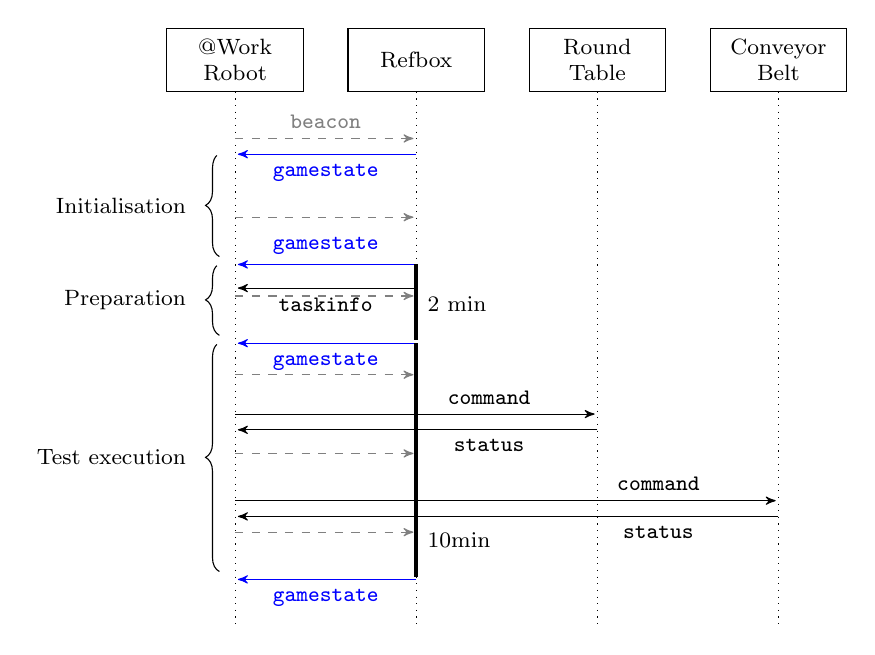
\begin{tikzpicture}[->,>=stealth',shorten >=1pt,auto,node distance=2.3cm,text centered, font={\footnotesize} ]
    \tikzstyle{element} = [draw=black, fill=white, rectangle, text width = 1.5cm, text centered, minimum height = 0.8cm, minimum width = 1.6cm]

    \tikzstyle{text_element} = [text width = 1.5cm, text centered]
    
    \node (ROBOT)[element]{@Work Robot};
    \node (REFBOX)[element, right of=ROBOT, fill=white, draw=black]{Refbox};
   \node (ROUNDTABLE)[element, right of=REFBOX]{Round Table};
  \node (CONVEYOR)[element, right of=ROUNDTABLE, fill=white, draw=black]{Conveyor Belt};
  
\coordinate (BELOW) at ($(ROBOT)+(0,-7.2cm)$);
\draw [dotted, -] (ROBOT) -- (ROBOT|-BELOW) ;
\draw [dotted, -] (REFBOX) -- (REFBOX|-BELOW) ;
\draw [dotted, -] (ROUNDTABLE) -- (ROUNDTABLE|-BELOW) ;
\draw [dotted, -] (CONVEYOR) -- (CONVEYOR|-BELOW) ;

\def \dist {1.0cm}
\coordinate (BEACON) at ($(ROBOT)+(0,-\dist)$);
\draw[->, dashed, gray] (BEACON) -- (BEACON-|REFBOX) node [midway] {{\tt beacon} } node [at end, anchor=center] (AUX){};

\def \dist {0.2cm}
\coordinate (START) at ($(AUX)+(0,-\dist)$);
\draw[->, blue] (START) -- (START-|ROBOT) node [midway] {{\tt gamestate} } node [at end, anchor=center] (AUX_1){};

\foreach \y in {2,...,6} 
       {\pgfmathtruncatemacro{\offset}{ \y * 1.3}
      \coordinate (BEACON) at ($(ROBOT)+(0,-\y)$);
       \draw[->, dashed, gray] (BEACON) -- (BEACON-|REFBOX) node [midway] {} node [at end, anchor=center] (AUX){};
} 

\def \dist {1.4cm}
\coordinate (START_PREP) at ($(START)+(0,-\dist)$);
\draw[->, blue] (START_PREP) -- (START_PREP-|ROBOT) node [midway, above] {{\tt gamestate}} node [at end, anchor=center] (AUX_1){};

\draw[-,decorate,decoration={brace,amplitude=5pt}] ($(START_PREP)-(2.5cm,-0.1cm)$) -- ($(START)-(2.5cm,0)$) node[midway, xshift=-0.3cm]{Initialisation};

\def \dist {0.3cm}
\coordinate (TASK) at ($(START_PREP)+(0,-\dist)$);
\draw[->] (TASK) -- (TASK-|ROBOT) node [midway] {{\tt taskinfo} } node [at end, anchor=center] (AUX_1){};

\def \dist {2.4cm}
\coordinate (START_GAME) at ($(START)+(0,-\dist)$);
\draw[->, blue] (START_GAME) -- (START_GAME-|ROBOT) node [midway] { {\tt gamestate} } node [at end, anchor=center] (AUX_1){};

\draw[-,decorate,decoration={brace,amplitude=5pt}] ($(START_GAME)-(2.5cm,-0.1cm)$) -- ($(START_PREP)-(2.5cm,0)$) node[midway, xshift=-0.3cm]{Preparation};

\draw[-, ultra thick] (START_PREP) -- (START_GAME) node [midway] {2 min};

\def \dist {5.4cm}
\coordinate (END_GAME) at ($(START)+(0,-\dist)$);
\draw[->,blue] (END_GAME) -- (END_GAME-|ROBOT) node [midway] { {\tt gamestate} } node [at end, anchor=center] (AUX_2){};

\draw[-,decorate,decoration={brace,amplitude=5pt}] ($(END_GAME)-(2.5cm,-0.1cm)$) -- ($(START_GAME)-(2.5cm,0)$) node[midway, xshift=-0.3cm]{Test execution};

\def \dist {0.9cm}
\coordinate (START_BELT) at ($(AUX_1)+(0,-\dist)$);
\draw[->] (START_BELT) -- (START_BELT-|ROUNDTABLE) node [midway, xshift=1cm] { {\tt command } } node [at end, anchor=center] (AUX_3){};

\def \dist {0.2cm}
\coordinate (END_BELT) at ($(AUX_3)+(0,-\dist)$);
\draw[->] (END_BELT) -- (END_BELT-|ROBOT) node [midway, xshift=1cm] { {\tt status } } node [at end, anchor=center] (AUX_1){};

\def \dist {0.9cm}
\coordinate (START_BELT) at ($(AUX_1)+(0,-\dist)$);
\draw[->] (START_BELT) -- (START_BELT-|CONVEYOR) node [midway, xshift=2cm] { {\tt command } } node [at end, anchor=center] (AUX_3){};

\def \dist {0.2cm}
\coordinate (END_BELT) at ($(AUX_3)+(0,-\dist)$);
\draw[->] (END_BELT) -- (END_BELT-|ROBOT) node [midway, xshift=2cm] { {\tt status } } node [at end, anchor=center] (AUX_1){};


\draw[-, ultra thick] (START_GAME) -- (END_GAME) node [midway, yshift=-1cm] {10min};

\end{tikzpicture}
% \caption{Sequence diagram of a complete competition run monitored by the referee box}
% \label{fig:refbox}
% \end{figure}
% \par
The TC provides a \aterm{Robot Operating System}{ROS} based interface of the referee box as well as
a reference implementation.
The Referee box implementation and its documentation is available under the following link:
\begin{center}
\url{https://github.com/robocup-at-work/atwork-commander}

\end{center}



% The publish/subscribe communication with the referee box and the external
% devices have to be mapped on the following topics:\note{We should not talk about @Work being a game, e.g. "gamestate". (Sven and Fred)}

% \begin{table}[h!]
% \centering
%  \begin{tabular}{|l|c|c|p{5.9cm}|}
%  \hline
%  Topic & Robot & Refbox & Remarks \\ \hline\hline
%  {\tt /atwork/refbox/gamestate} & S & P & {\tt uint8 gamestate \newline
% uint8 PREPERATION  = 0\newline
% uint8 RUNNING\_TASK = 1\newline
% uint8 PAUSE    = 2  \newline
% uint8 END\_TASK     = 3\newline
% uint8 STOP     = 4 }\\ \hline
%   {\tt /atwork/refbox/beacon} & P & S & {\tt
%   geometry\_msgs/Pose2D position \newline
% string  current\_action } \\ \hline
%    {\tt /atwork/refbox/taskinfo } & S & P & {\tt BNT[] bnt\_tasks \newline
% BMT[] bmt\_tasks  \newline
% BTT[] btt\_tasks } \\ \hline
%    {\tt /atwork/refbox/[device]/command} & P & S & {\tt int8 state \newline
% int8 ERROR        = -1 \newline
% int8 NOT\_RUNNING  = 0 \newline
% int8 RUNNING      = 1   }\\\hline
%    {\tt /atwork/refbox/[device]/status  } & S & P & {\tt int8 state \newline
% int8 ERROR        = -1 \newline
% int8 NOT\_RUNNING  = 0 \newline
% int8 RUNNING      = 1   }\\\hline
%  \end{tabular}
%   \label{tab:RefBoxTopics}
%  \caption{Referee box topics}
% \end{table}
%
% \begin{table}[h!]
% \centering
%  \begin{tabular}{|l|p{6.3cm}|}
%  \hline
%  Message types & Remarks \\ \hline\hline
%  {\tt Atworkobject} & {\tt uint8 name\newline
% uint8 F20\_20\_B = 0 \newline
% uint8 F20\_20\_G = 1 \newline
% uint8 S40\_40\_B = 2 \newline
% uint8 S40\_40\_G = 3 \newline
% uint8 M20\_100  = 4 \newline
% uint8 M20      = 5 \newline
% uint8 M30      = 6 \newline
% uint8 R20      = 7 \newline
% \revdel{uint8 V20      = 8} \newline
% string destination }\\ \hline
%
%  {\tt BNT} &  {\tt Waypoint[] waypoints }\\ \hline
%
%  {\tt BMT} &  {\tt string   startplace \newline
% string[] pickObjects \newline
% string   destination }\\ \hline
%
%   {\tt BTT} &  {\tt string destination  \newline
% AtworkObject[] objects }\\ \hline
%    {\tt Waypoint  } &  {\tt string position \newline
% uint8  orientation \newline
% uint8  WEST  = 0 \newline
% uint8  EAST  = 1 \newline
% uint8  SOUTH = 2 \newline
% uint8  NORTH = 3 \newline
% uint32  duration  }\\\hline
%  \end{tabular}
%  \caption{Refere box auxiliary message types \todo{can we provide a repository where the message files are stored? And make it consistent with items in Table \ref{tab:manipulation_objects} and \ref{tab:manipulation_objects_rockin}. And add the missing test like PPT, CBT, etc.}}
%   \label{tab:RefBoxAUX}
% \end{table}
%
% Table~\ref{tab:RefBoxAUX} summarizes the auxiliary types embedded in
% the referee box messages. A detailed description of the referee box-API is given in the
% corresponding documentation available on \todo{???????????????}.

\par
The referee box visualizes the current state of the competition run, time measurements, the task specification and robot positions for visitors. Team information (name, affiliation, contact information) are given too in this context.

%\todo{NICO: add maybe some screenshots from the referee box, also make a reference to the FESTO referee box}
\clearpage

\section{Design of the Environment}
\label{sec:ArenaDesign}

The competition is held in an arena resembling an example layout of industrial manufacturing facilities. 
The arena is a static 2D environment consisting of walls, tables and obstacles with a size of atleast 10 m$^2$ and not more than 120 m$^2$. 
An example layout is shown in fig. \ref{fig:arena_example}.

\begin{figure} [h!]
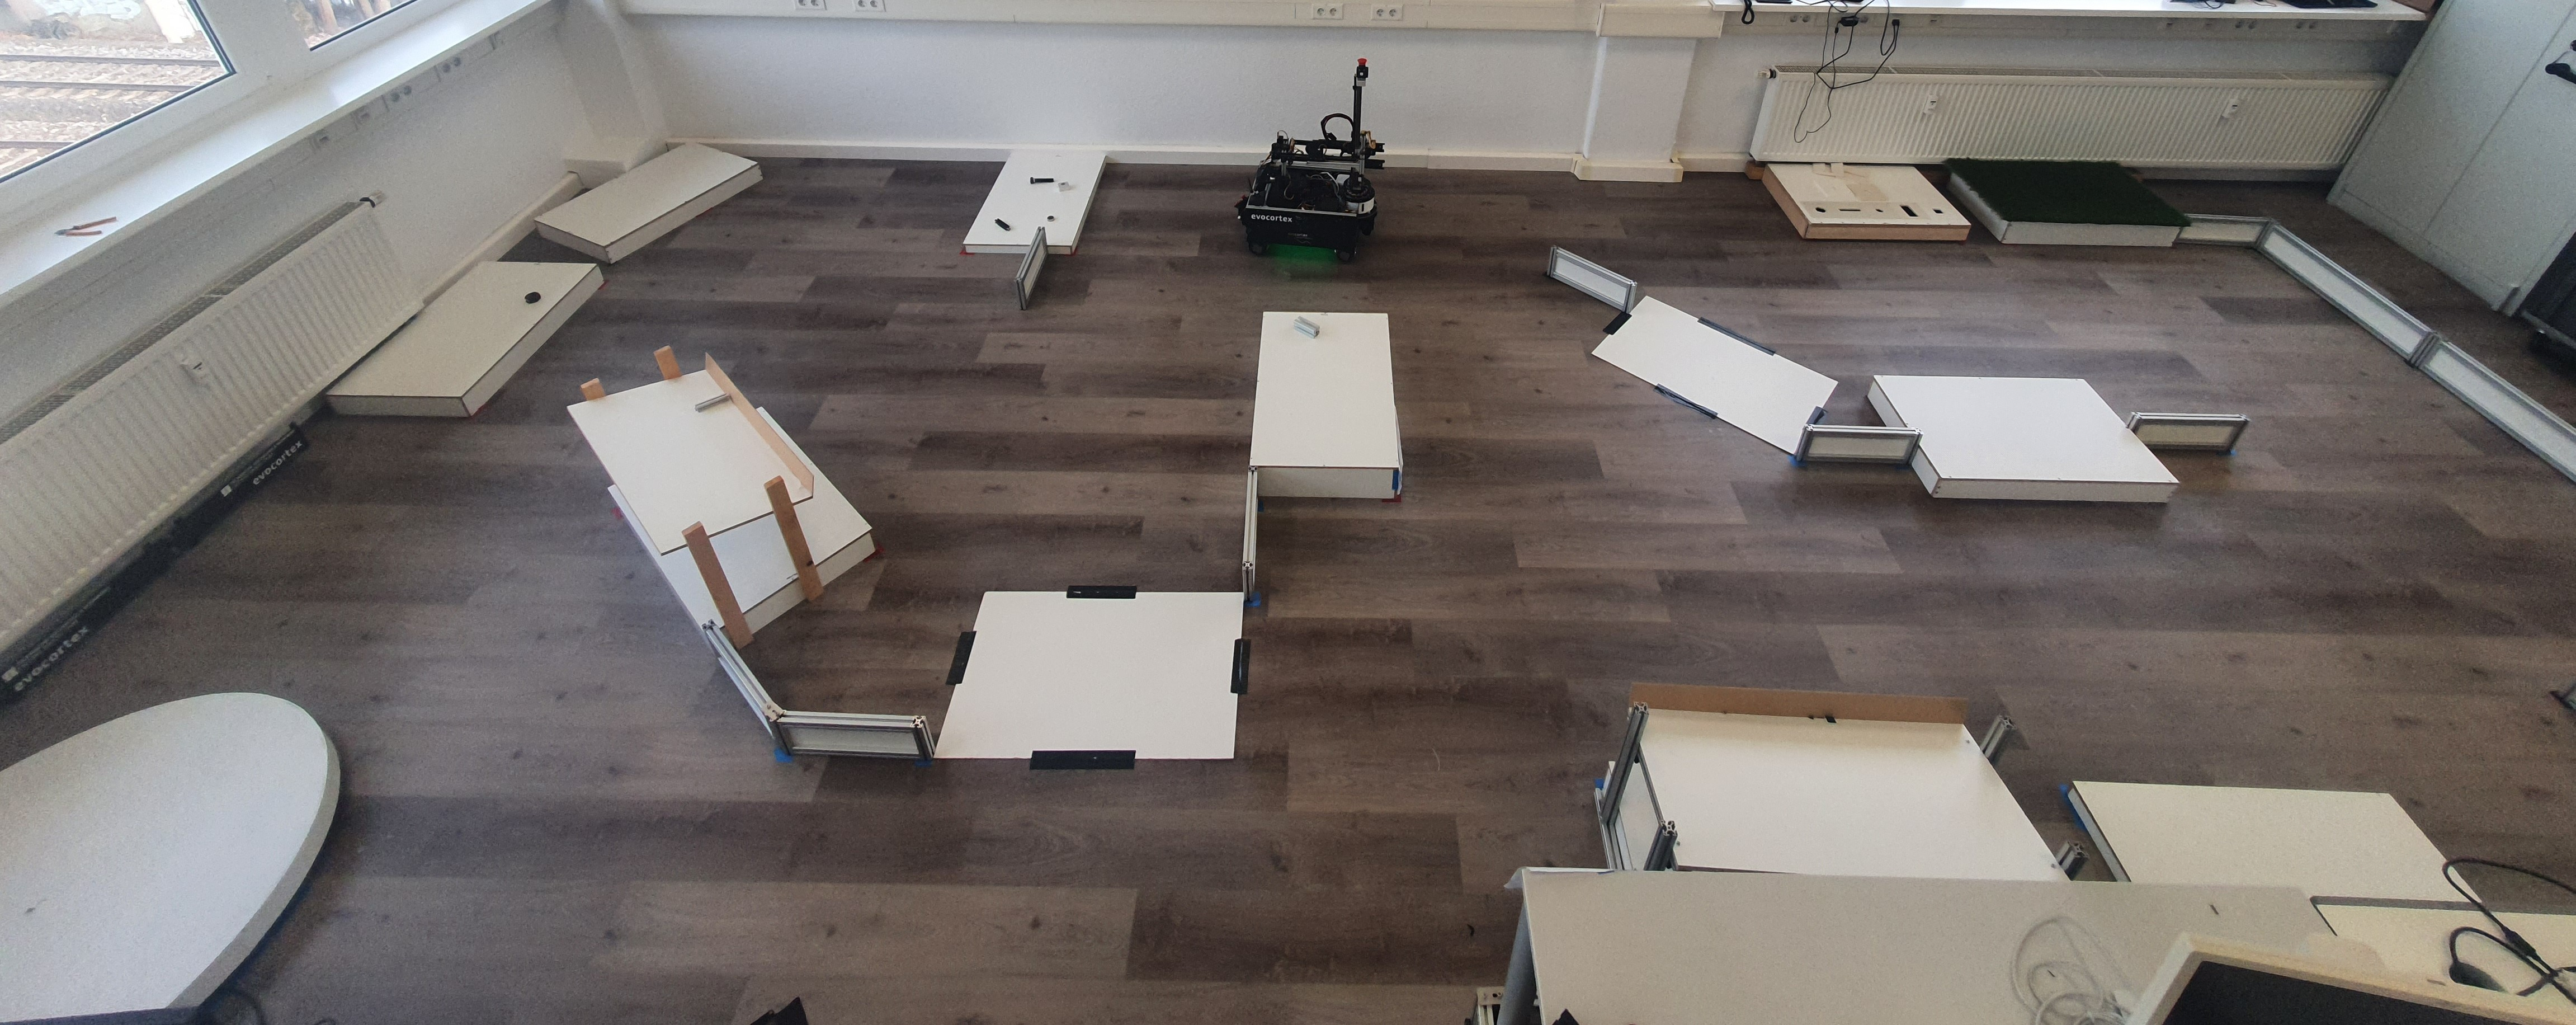
\includegraphics[width= \textwidth ]{./images/general_rules/arena_example.jpg}
\caption{An exemplary setup of a \RCAW environment.}
\label{fig:arena_example}
\end{figure}

Layouts may include rooms and hallways to create more realistic scenarios.
Service areas (see section \ref{ssec:serviceareas}) mark the locations for robots to perform tasks.
Each requested service area must be accessible via atleast one path of 80 cm width.

\begin{figure} [h!]
\centering
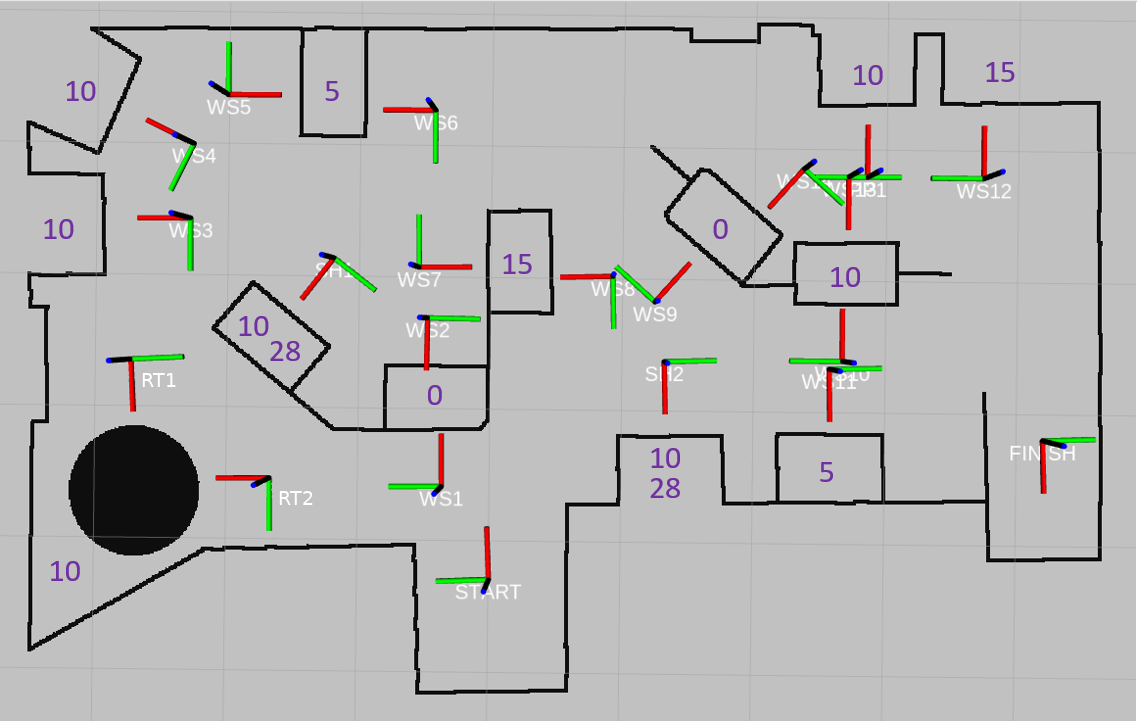
\includegraphics[width= 0.8\textwidth ]{./images/general_rules/arena_map_annotated}
\caption{Annotated 2D map of the environment in fig. \ref{fig:arena_example}}
\label{fig:arena_map_annotated}
\end{figure}

Each competition has a new and unique layout designed by the actual TC members.
It should feature:
\begin{itemize}
\item Area 10 m$^2$ - 120 m$^2$
\item Minimum distance between arena elements atleast 80 cm 
\item Widespread service areas entailing robot movements
\item Multiple paths between service areas
\item Start and Finish areas
\end{itemize}


\subsection{Service Areas} 
\label{subsec: serviceareas}

A service area indicates a location for a robot where tasks (e.g. picking or placing objects) have to be performed.
Such a location is usually a table with a flat white top (see fig. \ref{fig:arena_example}), but can also be a rotating table, shelf, precise placement station or any other type needed for a specific task.
In order to successfully reach a service area, robots must position themselves in front of the service area in a way that allows manipulation of the objects of interest. To enable robots to reach such a position, a rectangular area with 80 cm width must be kept free of obstacles (see fig. \ref{fig:arena_service_area_free}). 

\begin{figure} [h!]
\centering
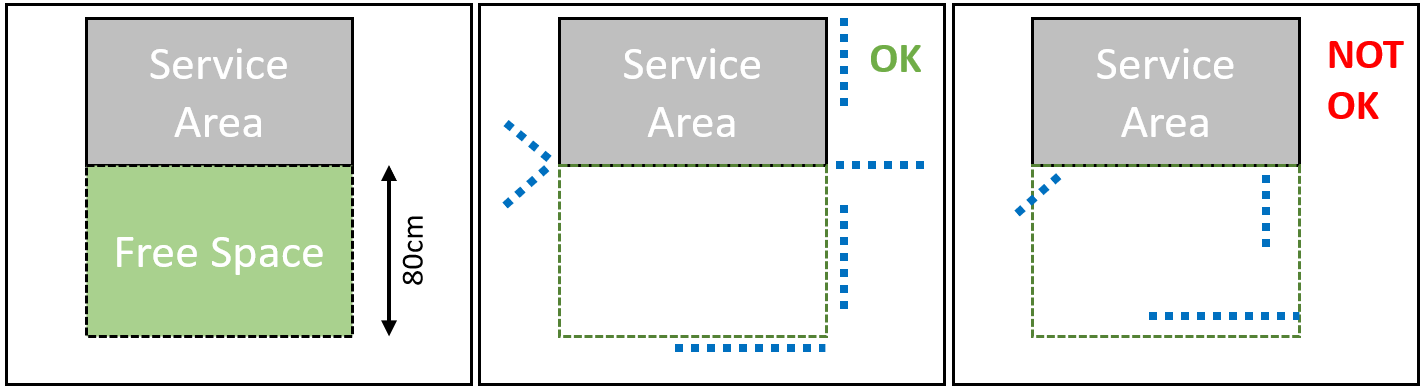
\includegraphics[width= 0.8\textwidth ]{./images/general_rules/arena_service_area_free_space}
\caption{Free Space in front of a service Area}
\label{fig:arena_service_area_free}
\end{figure}

The arena layout must define where the "front" of a table is.
Figure \ref{fig:arena_map_annotated} gives an example for the definition of the position of each service area, marking them as WSx (Workstation x), SHx (Shelf x) and CBx (Conveyor Belt x). The orientation only indicates the direction of the service area. It does not specify the robot's heading, which may be chosen by teams according to their individual robot design.

Tables that can be used from both sides (see fig. \ref{fig:arena_example}) are sometimes defined as two seperate workstations (e.g. WS5 & WS6). However, manipulation of a service area requires the robot to have its center in the rectangular area defined in fig. \ref{fig:arena_service_area_free}. This means that manipulation of the opposite service area is NOT allowed (see \ref{ssec:ManipulationZone}), even though it would be physically possible.
This rule also applies to the two positions for the rotating table (CB1 and CB2).
This makes smaller physical layouts possible that still provide the ability to create complex navigation challenges due to the amount of locations to visit.

Two special service areas are the START and FINISH positions. Both are rectangular areas for the robot to be positioned at the start or the end of a run. The service areas are marked using tape that may be crossed and are optionally equipped with light barriers used for time keeping.


\subsection{Walls and virtual Walls}
\label{subsec: Walls and virtual Walls}

The arena consists of outer and inner walls used to build structures, create obstacles or function as protection barriers for teams and viewers. Walls may be either physical (plank) or virtual (tape).
The arena is completely enclosed by walls (both types!), meaning robots are not allowed to exit the arena during a run.

The height of a physical wall must be not less than 20 cm and no more than 40 cm.
Most walls have a uniform main color (white), but may be enforced by metal (aluminum framework) and decorated with sponsor logos or ads.

Virtual walls are made of red and white tape (Tesa signal red/white) of 5 cm width. This tape may never be crossed during a run and is mainly used to close gaps in the physical outside walls.

\begin{figure} [h!]
\centering
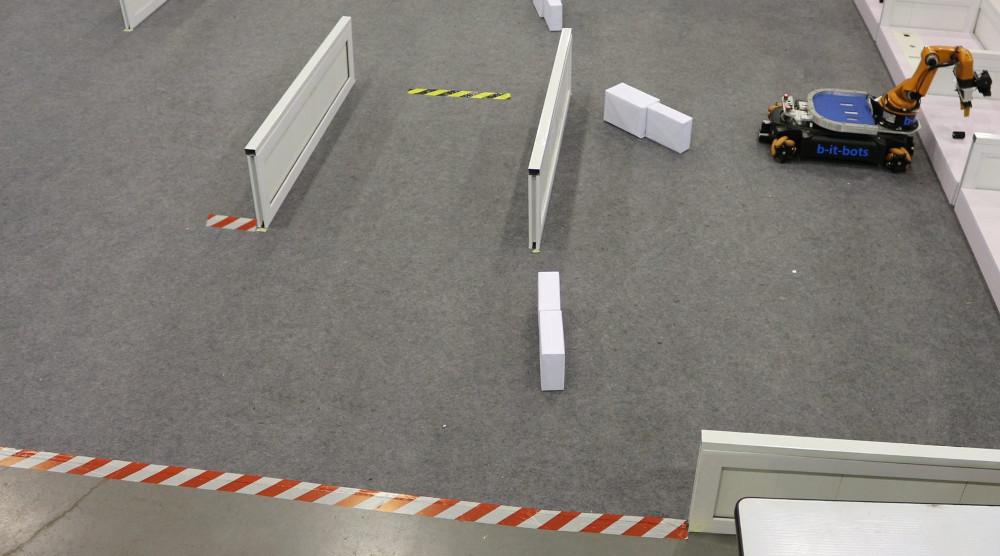
\includegraphics[width= 0.7\textwidth ]{./images/general_rules/barrier_tapes_in_china15.jpg}
\caption{Example of barrier tape used during \RC 2015. The red/white tape is used to indicate virtual walls , while the yellow/black one denotes a virtual fence.}
\label{fig:walls_and_virt_walls}
\end{figure}

Figure \ref{fig:walls_and_virt_walls} also shows black and yellow tape (Tesa signal black/yellow). 
This tape is referred to as 'Barrier Tape' and marks virtual fences. 
Such tapes are mainly used inside the arena to add obstacles.


\subsection{Obstacles}
\label{subsec: Obstacles}

In addition to the static arena elements, semi-dynamic obstacles may be placed inside the arena before a competition run begins. 
The position of such obstacles is decided by the referees during the setup phase of the run and randomized between different run types.

Obstacles may block paths partly or completely, as long as all active service areas are still reachable.
There are three main obstacle placement types:

\begin{itemize}
\item \textbf{Blocking:} 
A narrow section is completely blocked by the obstacle, which means that no robot can physically pass it ($<$ 20 cm).

\item \textbf{Semi-Blocking:} 
The obstacle reduces the distance between arena elements below the minimum width for a path. The path therefore counts as blocked, meaning that there must exist another valid path to all active service areas. Robots are still allowed to use all paths if they fit through the smaller gaps.

\item \textbf{Non-Blocking:}
The obstacle adds or enlarges an arena element but keeps all paths intact.
\end{itemize}

Obstacles can be either physical or virtual.
Physical obstacles measure atleast 2 x 2 x 20 cm (l x b x h) and may be made of any non-transparent, firm material (wood, metal). Some examples are bins, shipping boxes and wall elements. Their color is not specified.
All physical obstacles are treated like any other arena element during a run, including the rules for collisions.

Virtual obstacles are marked using the Barrier Tape from section \ref{subsec: Walls and virtual Walls}. 
These virtual fences recently have been introduced to the league, which is why collisions with them are treated differently (see REF SCORING).

\subsection{Arena Element Specifications}
\label{subsec: Arena Element Specifications}

\subsubsection{Markup Tape}

LEANDER

Used to mark tables, start fin etc.

\subsubsection{Floor}
The floor is made of some firm material. Examples include floors made of concrete, screed, timber, plywood, chipboard, laminated boards, linoleum, PVC flooring, or carpet. Some examples are illustrated in Figure \ref{fig:example_floors}. Floors may neither be made of loose material of any kind (gravel, sand, or any material which may damage the functioning of the robot's wheels) nor may such material be used on top of the floor. Liquids of any kind are not allowed. The floor may have spots of unevenness of up to 1 cm in any direction (clefts, rifts, ridges, etc.).

\begin{figure} [h!]
\begin{center}
\subfloat{
\includegraphics[height = 2cm]{./images/general_rules/example_floor_1.jpg}} \hspace{0.1cm}
\subfloat{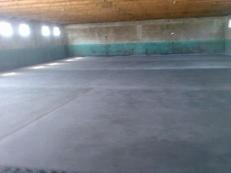
\includegraphics[height = 2cm]{./images/general_rules/example_floor_2.jpg}} \hspace{0.1cm}
\subfloat{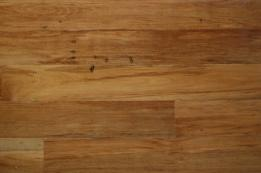
\includegraphics[height = 2cm]{./images/general_rules/example_floor_3.jpg}} \hspace{0.1cm}
\subfloat{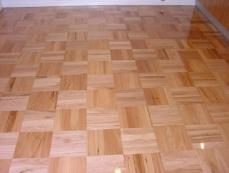
\includegraphics[height = 2cm]{./images/general_rules/example_floor_4.jpg}} \hspace{0.1cm}
\subfloat{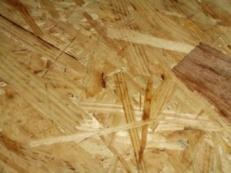
\includegraphics[height = 2cm]{./images/general_rules/example_floor_5.jpg}}\\
\subfloat{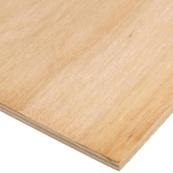
\includegraphics[height = 2cm]{./images/general_rules/example_floor_6.jpg}} \hspace{0.1cm}
\subfloat{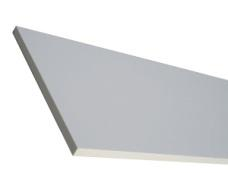
\includegraphics[height = 2cm]{./images/general_rules/example_floor_7.jpg}} \hspace{0.1cm}
\subfloat{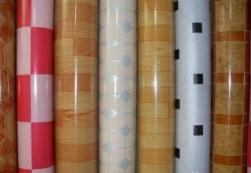
\includegraphics[height = 2cm]{./images/general_rules/example_floor_8.jpg}} \hspace{0.1cm}
\subfloat{
\includegraphics[height = 2cm]{./images/general_rules/example_floor_9.jpg}} \hspace{0.1cm}
\subfloat{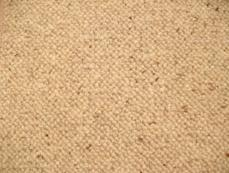
\includegraphics[height = 2cm]{./images/general_rules/example_floor_10.jpg}}
\end{center}
\caption{Examples of floors that can be used for \RCAW arenas.}
\label{fig:example_floors}
\end{figure}



\subsubsection{Workstations - TODO}

However, from 2020 on and in order to make the competition more realistic, the heights of the service areas will be variable, allowing the OC to adjust them before each test run.
If a service area has a height of zero cm, a tape will mark the area (see Figure \ref{fig:barrier_tape_0cm}).
The tape will be on the floor and will be blue/white striped.
The surounded area may be covered by a white sheet of paper fixed by the tape.
The OC is responsible to replace it in case of pollution or tears.
This tape may be crossed, and does not count as a collision.
If the robot touches a manipulation object while navigating, this will be handled as a collision.

\begin{figure} [h!]
\begin{center}
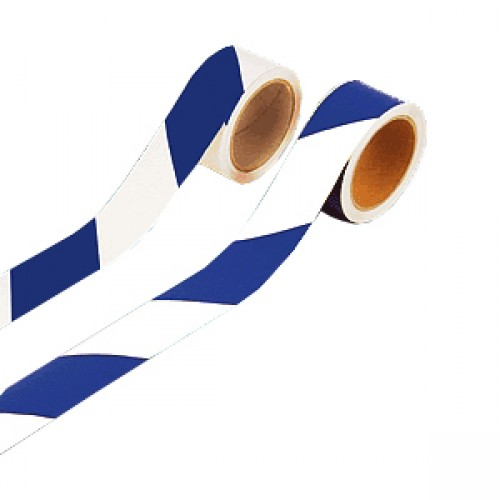
\includegraphics[height = 2.5cm]{./images/barrier_tape_0cm_area.jpg}
\end{center}
\caption{Barrier tape used to mark service areas with 0 cm height.}
\label{fig:barrier_tape_0cm}
\end{figure}

Until 2017, service areas have always been represented by white coloured surfaces with no other decoy objects on it than the official ones in Tables \ref{tab:manipulation_objects} and \ref{tab:manipulation_objects_rockin}.
However, this does not represent real life scenarios.
The robot might have to pick objects from different colored or dirty places. Also there could be other industrial items on the surface area that the robot must avoid.
In order to make the operating environment more realistic, different kinds of arbitrary surfaces (Figure \ref{fig:ast_surface_example}) with decoy industrial items (Figure \ref{fig:ast_example}) have been introduced.
To facilitate the participation of newer teams that are yet focused on more basic functionalities, the integration of arbitrary surfaces is by now limited to:
\begin{itemize}
\item One service area during the BTT1.
\item Two service areas during the BTT2.
\item Two service areas during the BTT3.
\item Three service areas during the final round.
\end{itemize}

\begin{figure}[h!]
\centering
\subfloat[]{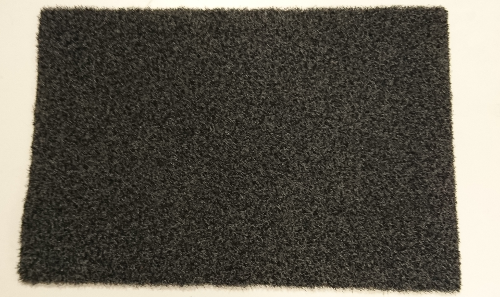
\includegraphics[width=.3\textwidth]{./images/Arbitrary_Surface_rug}}
\hspace{0.5cm}
\subfloat[]{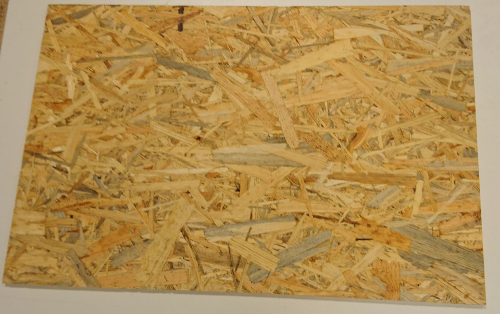
\includegraphics[width=.3\textwidth]{./images/Arbitrary_Surface_wood}}
\hspace{0.5cm}
\subfloat[]{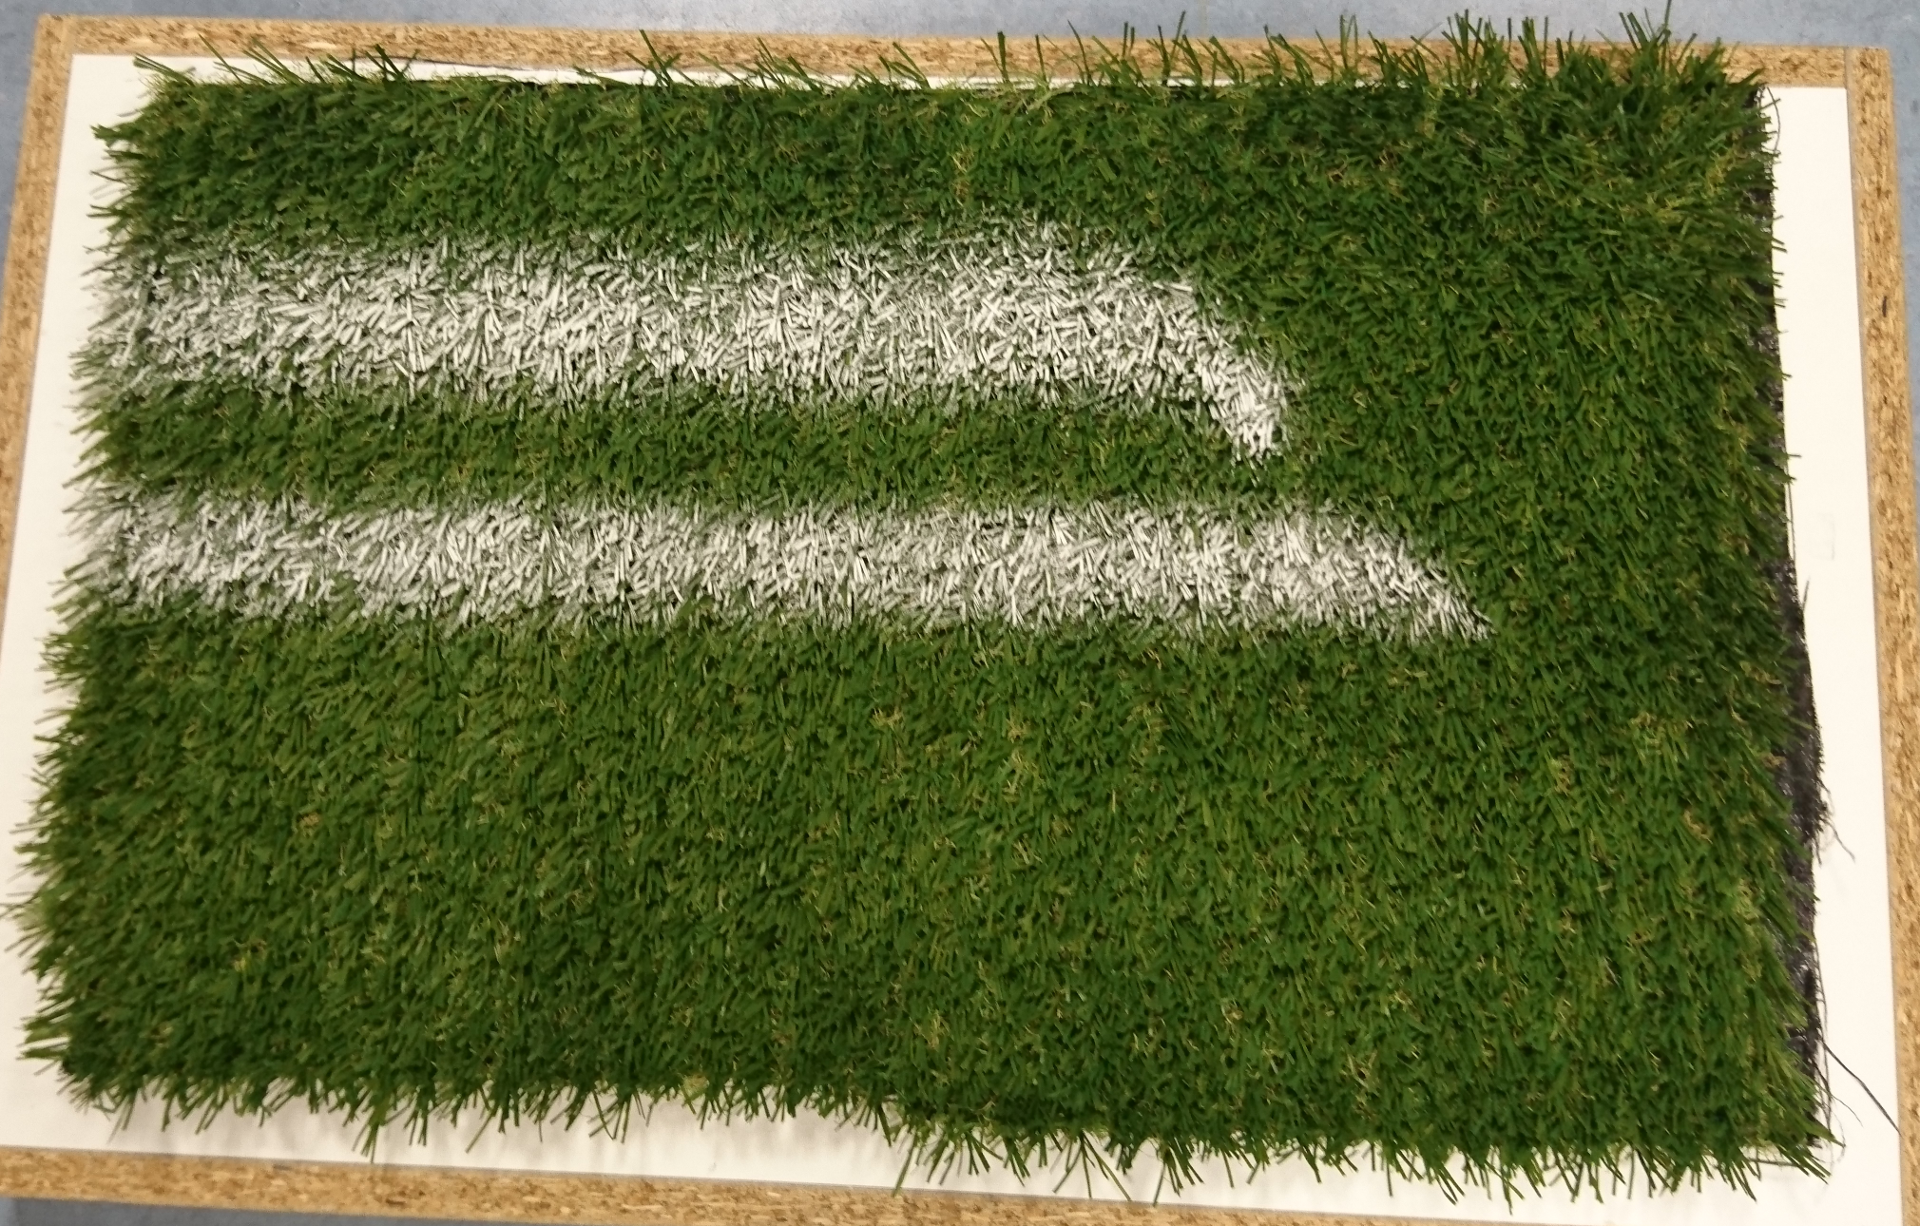
\includegraphics[width=.3\textwidth]{./images/Arbitrary_Surface_grass}}\\
\subfloat[]{\includegraphics[width=.3\textwidth]{./images/Arbitrary_Surface_fake_wood_1}}
\hspace{0.5cm}
\subfloat[]{\includegraphics[width=.3\textwidth]{./images/Arbitrary_Surface_fake_wood_2}}
\caption{Examples of arbitrary surfaces used for service areas.}
\label{fig:ast_surface_example}
\end{figure}

\begin{figure}[h!]
\begin{center}
\subfloat[]{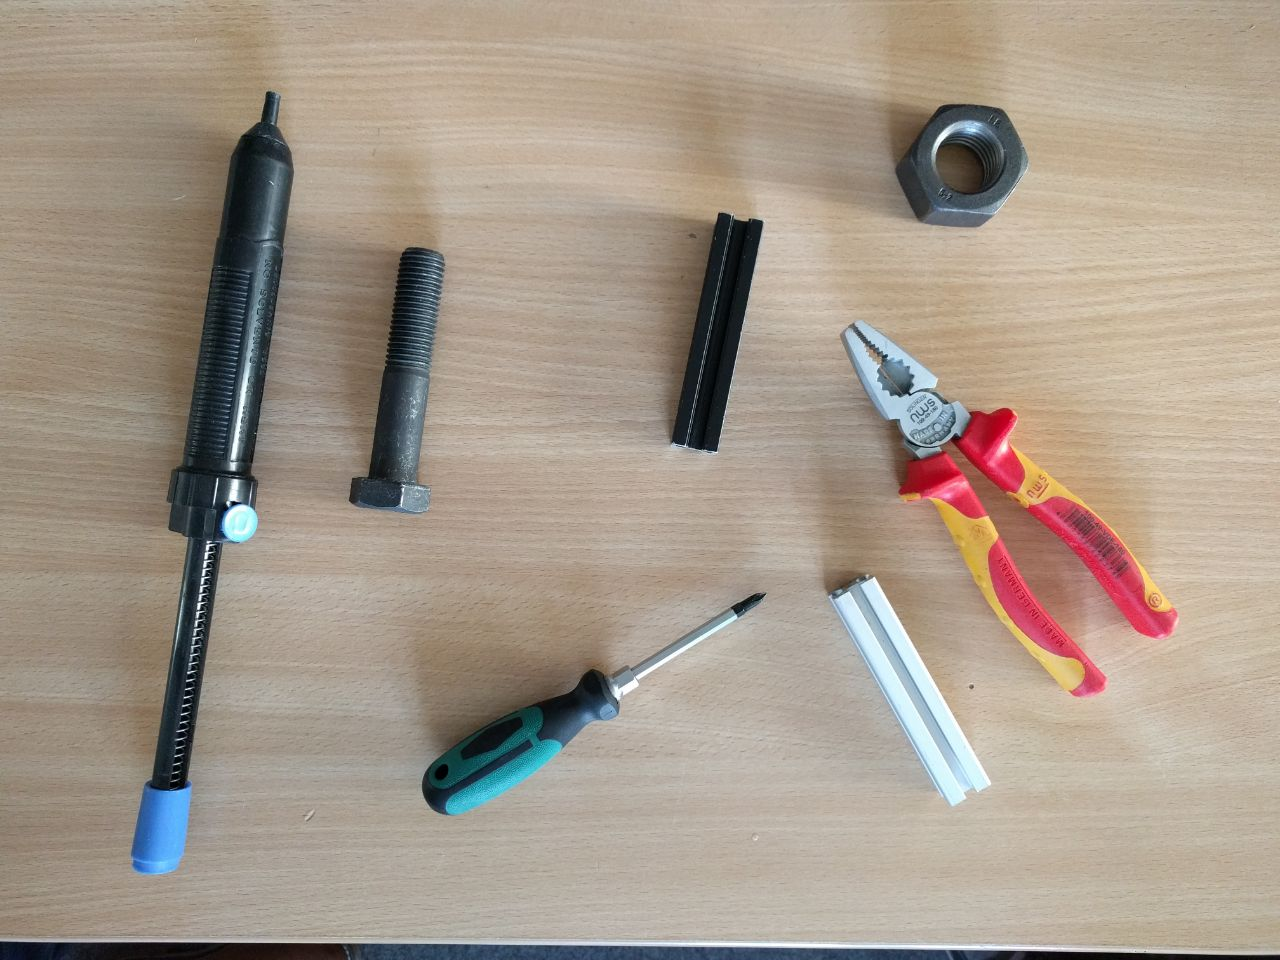
\includegraphics[height = \textwidth/3]{./images/realisticWorkingDeskI.jpeg}}
\hspace{0.5cm}
\subfloat[]{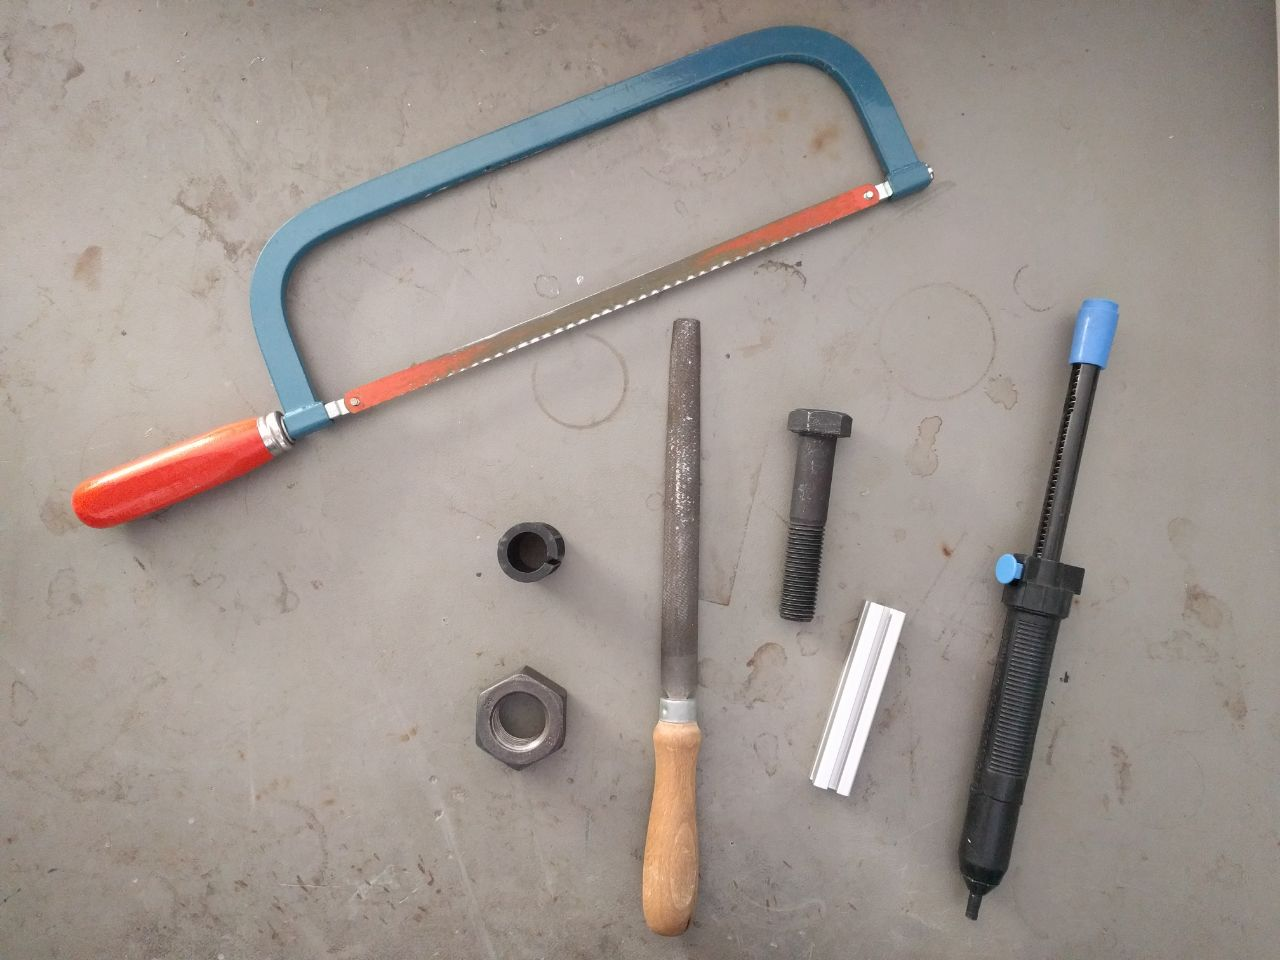
\includegraphics[height = \textwidth/3]{./images/realisticWorkingDeskII.jpeg}}
\end{center}
\caption{Examplary configuration of the working desks}
\label{fig:ast_example}
\end{figure}





%\subsection{Racks}
%Service areas, e.g. loading and unloading areas, may foresee the use of racks. Objects to be delivered or removed from racks have to be placed or picked up from the top. The height of the racks should be not lesser than 5 cm and not more than 40 cm. The color for the top surface of racks is a bright uniform color such as white or light gray, unless a test specifies a different color. The top surface of the rack may be specially designed in order to serve specific purposes, e.g. holding objects.

\subsubsection{Shelves}\label{sec:Shelves}
Service areas may foresee the use of shelves and shelf units as depicted in Figure~\ref{fig:shelf}. Objects to be delivered or removed from shelves have to be placed or picked sideways. The height of the shelves should be not lesser than 5 cm and not be more than 40 cm.
The shelf surface may be specially designed in order to serve specific purposes, e.g.\, holding objects.

\begin{figure} [h!]
\centering
\subcaptionbox{A shelf with two levels and uniform colored surfaces.}{%
  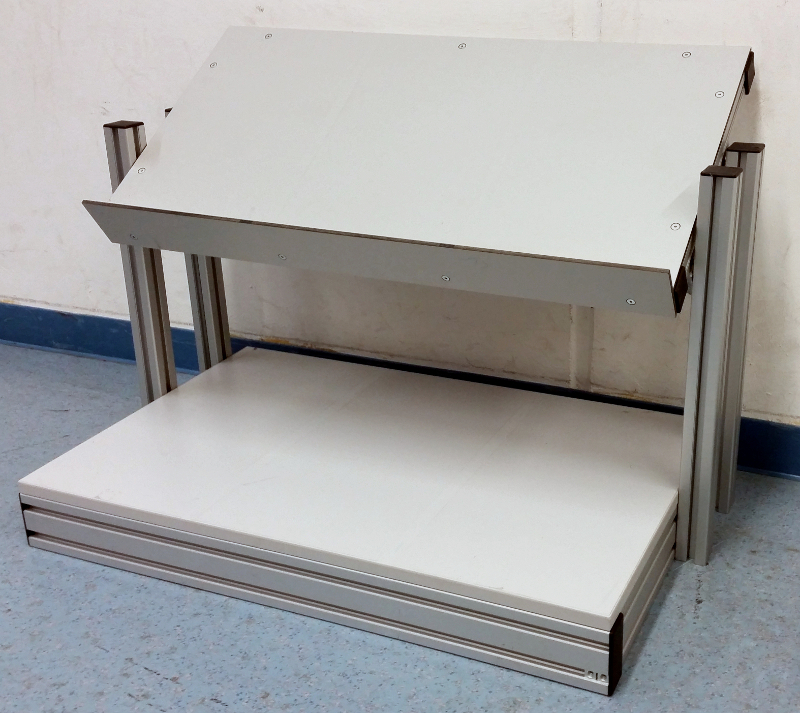
\includegraphics[width=0.4\textwidth ]{./images/shelf.jpg}%
}%
\subcaptionbox{Technical draw of shelf configuration.}{%
  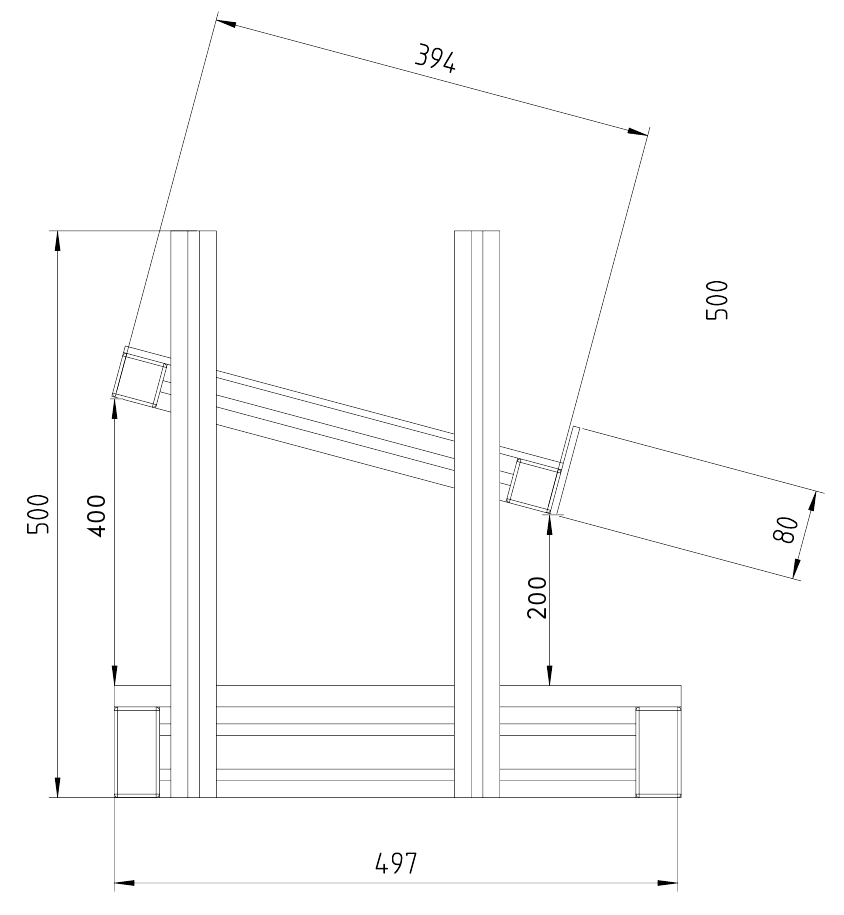
\includegraphics[width=0.4\textwidth ]{./images/SketchShelf.jpeg}%
}
\caption{Exemplary shelf and generic technical drawing.}%
\label{fig:shelf}
\end{figure}

\subsubsection{Rotating Turntable - TODO}

\subsubsection{Containers - Move to manipulation?}
As in many industrial settings, the \RCAW environment may be equipped with several containers (see Figure~\ref{fig:containers}). They can store any kind of manipulation object defined in Section~\ref{ssec:ManipulationObjects}. Robots are supposed either to grasp one or multiple objects out of containers or to place previously grasped objects into them. Several containers can be present in the environment and are always associated with a service area. That means that the container itself will be placed on top and within the manipulation zone defined in Section~\ref{ssec:ManipulationZone}.
It is also possible that more than one container is placed on top of a single service area.
The constraints defined in Section~\ref{ssec:ManipulationZone} apply also to the containers.

Currently, a container itself does to not need to be manipulated or transported by the robot.

\begin{figure} [h!]
\begin{center}
\subfloat[blue]{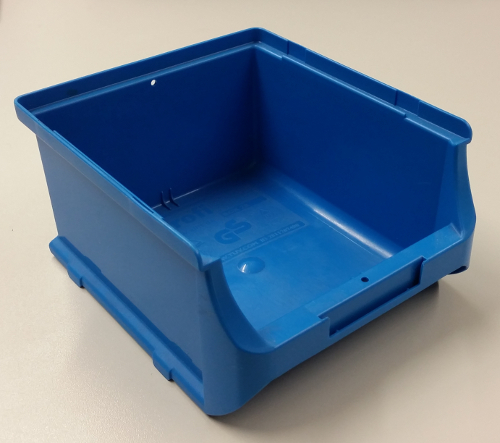
\includegraphics[height = 3cm]{./images/container_blue.jpg}} \hspace{1cm}
\subfloat[red]{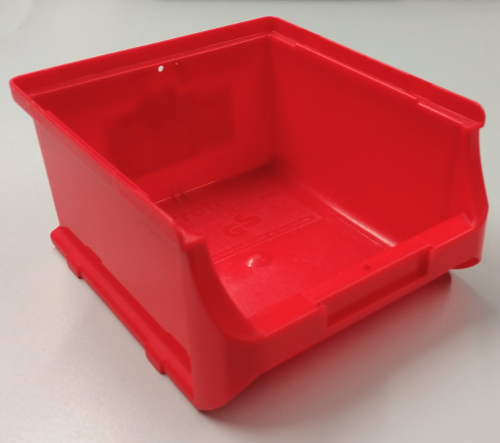
\includegraphics[height = 3cm]{./images/container_red.jpg}}
\end{center}
\caption{Containers can be used for grasping objects out or placing objects into them.}
\label{fig:containers}
\end{figure}


\section{Design of Navigation Tasks} \label{sec:NavigationTasks}
Every task has some navigation involved in it. Successful navigation will be awarded in every test according to Table \ref{tab:InstancePoints}. If not defined differently in the respective test, a navigation is successful when the robot reached the service area as defined in section \ref{ssec:Navigating}. 

\textbf{REMARK:} Since 2020 the BNT test is removed from the set of tests done at the competition. Remark that points for reaching service areas are given in all tests, so that teams which are only able to navigate with their robot can still achieve points in all tests.


\subsection{Reaching a Service Area} \label{ssec:Navigating}
A service area counts as successfully reached if the robot would be able to manipulate the service area it is standing on. The manipulation range will be subjectively evaluated by the referees.


\section{Design of Manipulation Tasks} \label{sec:ManipulationTasks}


\subsection{Manipulation Zone} \label{ssec:ManipulationZone}
The manipulation zone defines the area where objects can be placed. Thereby, the following constraints need to be satisfied:
\begin{itemize}
	\item The maximum depth of the manipulation zone is 20 cm.
	\item The minimum distance between objects to each other is 2 cm.
	\item The minimum distance of the beginning of the manipulation zone to a wall is 10 cm.
	\item There as an offset of 2 cm from the border of the service area to the manipulation zone.
\end{itemize}
Note, the constraints do not permit, that objects can be partially occluded dependent on the viewpoint.
\begin{figure} [h!]
\centering
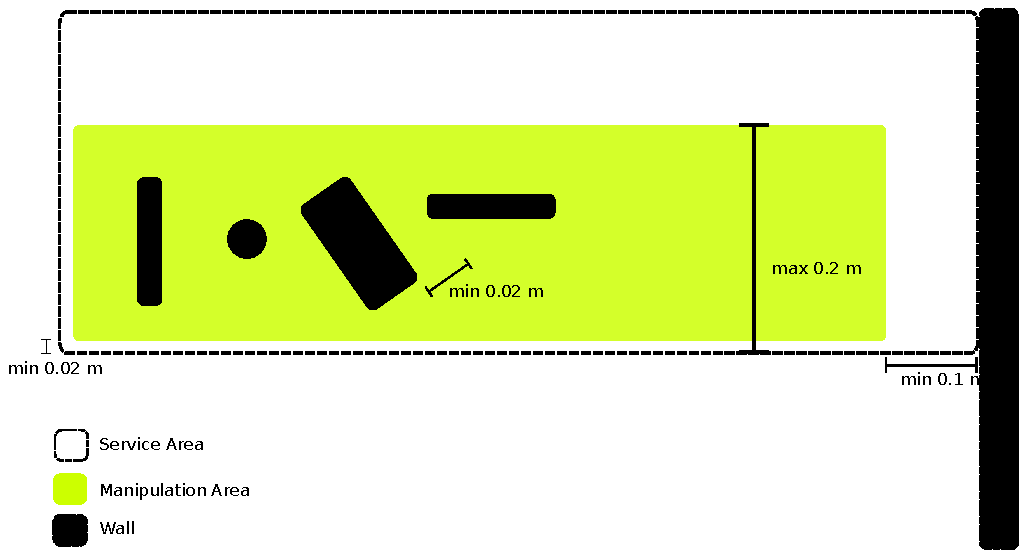
\includegraphics[width=1.0\textwidth ]{./images/manipulation_zone.pdf}
\caption{Manipulation zone: the green color indicates the area where objects can be placed on a service area by the referees.}
\label{fig:manipulation_zone}
\end{figure}


\subsection{Manipulation Objects} \label{ssec:ManipulationObjects}
The manipulation objects in \RCAW shall include a wide range of objects relevant in industrial applications of robotics. They eventually cover any raw material, (semi-)finished parts or products as well as tools and possibly operating materials required for manufacturing processes.
\par
The intention is to start with a simple set of objects of different shapes and colors. Every year, the spectrum shall then be widen in at least one aspect. The initial set of objects includes basic standard screws and nuts with various sizes and masses as shown in Table~\ref{tab:manipulation_objects} and Table~\ref{tab:manipulation_objects_rockin}. Objects of one kind can slightly vary e.g. considering the surface.

For the placement of manipulation objects the following terms are used:

\begin{itemize}
\item Position: point within 2D coordinate system of a service area,
\item Rotation: rotation around vertical axis of a service area,
\item Orientation: rotation around horizontal axes of a service area, i.e. whether the object is standing upright or lying on its side
\item Pose: combination of position, rotation and orientation.
\end{itemize}

\newcommand{\imageView}[1]{\includegraphics[width=2cm, valign=c]{#1}}
{
\newcommand{\rowpadding}{0.4cm}
\setlength\extrarowheight{\rowpadding}
\begin{table}[p]
\begin{tabular}{|c|c|c|m{6cm}|}
\hline
Object & Symbolic Description & Mass & Details \\
\hline
\imageView{./images/F20_20_B.jpg} & \texttt{F20\_20\_B} & 49 g & Small aluminium profile (black)\newline
 Height: 20 mm \newline
 Width: 20 mm \newline
 Length: 100 mm \\ [\rowpadding]
\hline
\imageView{./images/F20_20_G.jpg} & \texttt{F20\_20\_G} & 49 g & Small aluminium profile (gray)\newline
 Height: 20 mm \newline
 Width: 20 mm \newline
 Length: 100 mm \\ [\rowpadding]
\hline
\imageView{./images/S40_40_B.jpg} & \texttt{S40\_40\_B} & 186 g & Big aluminium profile (black)\newline
 Height: 40 mm \newline
 Width: 40 mm \newline
 Length: 100 mm \\ [\rowpadding]
\hline
\imageView{./images/S40_40_G.jpg} & \texttt{S40\_40\_G} & 186 g & Big aluminium profile (gray)\newline
 Height: 40 mm \newline
 Width: 40 mm \newline
 Length: 100 mm \\ [\rowpadding]
\hline
\imageView{./images/M20_100.jpg} & \texttt{M20\_100} & 296 g & Screw\newline
 ISO 4014 \newline
 M20 \newline
 Length: 100 mm \\ [\rowpadding]
\hline
\imageView{./images/M20.jpg} & \texttt{M20} & 56 g & Small nut\newline
 ISO 4032 \newline
 M20 \\ [\rowpadding]
\hline
\imageView{./images/M30.jpg} & \texttt{M30} & 217 g & Big nut\newline
 ISO 4032 \newline
 M30 \\ [\rowpadding]
\hline
\imageView{./images/R20.jpg} & \texttt{R20} & 14 g & Plastic tube\newline
 Inner diameter: 20 mm \newline
 Outer diameter: 30 mm \newline
 Length: 45 mm \\ [\rowpadding]
\hline
%\imageView{./images/V20.jpg} & \texttt{V20} & 14 g & Inner diameter: 20 mm \newline
%Outer diameter: 30 mm \newline
%Length: 45 mm \\
%\hline
\end{tabular}
\caption{\RCAW manipulation object set.}
\label{tab:manipulation_objects}
\end{table}


\begin{table}[p]
\begin{tabular}{|c|c|c|m{6cm}|}
\hline
Object & Symbolic Description & Mass & Details \\
\hline

\imageView{./images/bearingBoxA.jpg} & \texttt{Bearing\_Box} & 102 g & Bearing box\newline
 Height: 25 mm \newline
 Width: 45 mm \newline
 Length: 50 mm \newline
 Inner diameter: 32 mm \\ [\rowpadding]
\hline

\imageView{./images/bearing.jpg} & \texttt{Bearing} & 42 g & Bearing\newline
 Height: 13 mm \newline
 Inner diameter: 15 mm \newline
 Outer diameter: 32 mm \\ [\rowpadding]
\hline

\imageView{./images/axis.jpg} & \texttt{Axis} & 40 g & Axis\newline
 Diameter: 27 mm \newline
 Length: 96 mm \\ [\rowpadding]
\hline

\imageView{./images/distanceTube.jpg} & \texttt{Distance\_Tube} & 5 g & Distance tube\newline
 Height: 10 mm \newline
 Inner diameter: 28 mm \newline
 Outer diameter: 32 mm \\ [\rowpadding]
\hline

\imageView{./images/motor.jpg} & Motor & 20 g & Motor\newline
 Diameter: 42 mm \newline
 Length: 87 mm \\ [\rowpadding]
\hline
\end{tabular}
\caption{RoCKIn manipulation object set.}
\label{tab:manipulation_objects_rockin}
\end{table}
}


\subsection{Grasping Objects} \label{ssec:GraspingObjects}
If not specified differently in a test, the following definition applies to decide if an object counts as being grasped from a service area.
\par
An object counts as grasped from a service area, when the object was moved outside of the source service area. Outside means, that the vertical projection of the object’s convex hull does not touch the service area any more.

\par
The last point shall enable to let the robot pick up an object in order to analyse its type, e.g. by holding it close to a camera on the robot.
\par
If the robot handles an object, but does not fulfill all points above, the object does not count as being grasped, and neither points for grasping a required object, nor penalty points for grasping an unspecified object are given. Still, if the object drops to the ground or an uncontrolled collision occurs, the normal penalty points apply.

\subsection{Placing Objects on Service Areas} \label{ssec:PlacingObjects}
If not specified differently in a test, a manipulation object counts as placed on a target service area if any part of the object is touching the surface of the service area and the object is not moving at the end of the run. An objects does not count as placed when it is dropped (e.g. dropped from a height above 5 cm). This is to avoid that robots throw objects and potentially harm people or property.
\par
The pose of the object on the service area can be chosen freely by the robot.

%\section{Overall Scenario and Variation Points}
%The following two figures illustrate the kind of arenas that can be built with the previously described components. Figure \ref{fig:example_map} shows an old arena configuration (from IROS 2012) as a topological map defining places and connections, while Figure \ref{fig:example_map_go13} shows an arena configuration (from German Open 2013) with only a few surrounding walls, more open space and a conveyor belt.

%\begin{figure}
%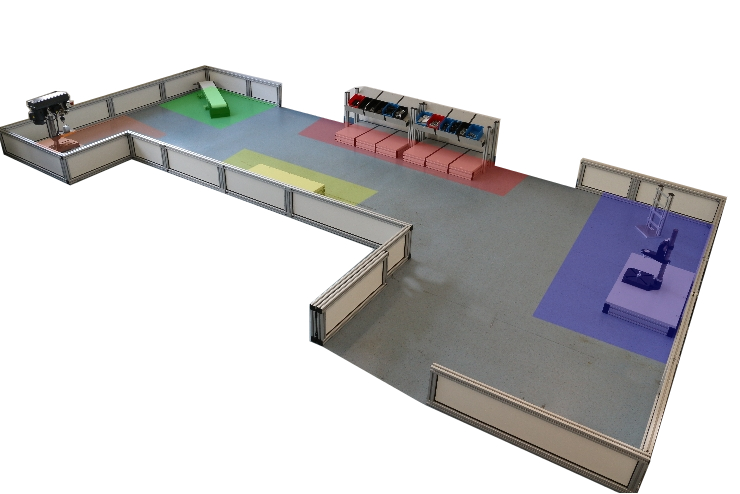
\includegraphics[width= \textwidth ]{./images/arena_brsu_spatial_areas.jpg}
%\caption{Illustration of one possible arena configuration. \todo{similar to Figure~\ref{fig:example_arena}. Delete one or put them together in a subfigure environment}}
%\label{fig:example_map_brsu}
%\end{figure}



\chapter{Tests}
% !TEX root = ../Rulebook.tex
\label{sec:Tests}

\section{General}

\subsection{Common Rules}
\label{ssec: Common Rules}


Unless stated other, the following rules apply to all test types:

\begin{itemize}
\item The order in which the teams have to perform will be determined by a draw from the OC.
\item Teams must not hardcode information gained from runs of previous teams.
\item A single robot is used.
\item The robot must not leave the arena.
\item The maximum objects a robot is allowed to carry is 3.
\item The robot has to start and end at the respective arena location (START, FINISH).
\item The robot will get the task specification from the AC.
\item Reaching succesfully a Service Area is rewarded as defined in \ref{tab:InstancePoints}.
\item The reward for reaching a Service Area will be only rewared once for a Service Area.
\item Service Areas count as succesfully reached as defined in section \ref{sec:ArenaDesign}.
\item Manipulation tasks count as successful as defined in \ref{ssec:GraspingObjects} and \ref{ssec:PlacingObjects}.
\item The score for this test will be calculated as defined in \ref{sec:ScoringAndRanking}.
\item Exact test specification is displayed in table \ref{tab:Instances}.
\end{itemize}


%\end{itemize}



%The actual competition contains of a set of so-called tests. 
%A test is specified in terms of it's purpose and focus, environment features and eventually manipulation objects involved. Further, a concrete specification of the task is given and the rules to be obeyed. 

%Each test has different variability dimensions. That is, which objects to be manipulated, how many locations to visit, from which height to grasp etc. The test instances for \YEAR are defined based on the general test description and can be seen in Section~\ref{sec:ScoringAndRanking}.




%Every test has some navigation to a service area involved in it. Successful navigation will be awarded in every test according to Table \ref{tab:InstancePoints}. A navigation to a service area is successful when the robot reached the service area as defined in section \ref{ssec:Navigating}. The rewarded points for navigation to a servie area will be only awarded once per service area.

\subsection{Grasping Objects} \label{ssec:GraspingObjects}

An Object counts as successfully grasped, if the robot grasps the correct Object of the correct Service Area and transport it out of the corresponding Service Area. In that case the Service Area has an infinite height.

A robot is allowed to grasps an incorrect Object as long as the Object don't leave the Service Area with his complete form. This enables a robot to grasp an Object to examine the Object with a camera. If an incorrect Object grasped and moved out of the Service Area it is counted as an incorrect Object Grasping.

If the Objects falls down from the platform, the robot drops the Object to the floor after leaving the Service Area or the Object falls on top of the Service Area from a height higher than $5\si{\centi\meter}$ while the grasping process it is counted as an Object Loss.

The grasping process starts when the Manipulator enters the Service Area und ends when it leaves the Service Area.

\subsection{Placing Objects} \label{ssec:PlacingObjects}

\textbf{General}

An Object counts as successfully placed, if the robot places an correct Object to a Manipulation Zone of the correct Service Area. The robot has to place the Object so that the Object is lying with his complete form inside the Manipulation Zone. The pose of the Object on the Manipulation Zone can be chosen freely by the robot.

There is a Placement Deduction that will be subtracted from the points of the successfull Grasping. The Placement Deduction will be applied at the following situations, if multiple situations happen while the same placing process the Placement Deduction will applied only once:

\begin{itemize}
	\item If the placed Object or the Manipulator touches another Object, Container or Decoy while the placing process at the Manipulation Zone 
	\item If the placed Object is not lying with his complete form within the Manipulation Zone at the end of the placement process
\end{itemize}

The placement process starts when the Manipulator with the Object enters the Service Area and ends when the placed Object doesn't move anymore and the Manipulator has left the Service Area. In these cases the Service Area has an infinte height.


If an Object is placed from a height higher than $5\si{\centi\meter}$ to the top of the Manipulation Zone it is considered as an Object Loss and no points are given for a successfull Placing.

If a placed Object is either incorrect or the corresponding Service Area is incorrect, the Placement is considered as an Incorrect Placement. If at this Incorrect Placement a Placement Deductions occurs then no additional penalty points will be added to the Incorrect Placement penalty.

\textbf{Shelf}

The Placement at the upper part of the Shelf has to be in the Manipulation Zone of the upper part of the shelf and it is allowed that the Object is moving down to the lower area of the upper part of the shelf after the placement. 


\textbf{Precision Placement}

A successfull Placement of the Object into the cavity will rewarded with a successfull Precision Placement. A successfull Precions Placement is if a  correct Object falls through the correct cavity tile. If the Object is not falling down through the cavity but is stuck in the cavity or is lying at the end of the run at the correct cavity it will be rewarded with an successfull Cavity Placement. However The Object has to be lying with his complete form within the correct cavity.

If an Object is placed on the wrong cavity tile then no points are given and in this case there is also no incorrect Object Placing penalty as long as the Object has to be placed at this Precision Table. If an Object is placed on a Precision Table that shouldn't be placed there, then the incorrect Object Placement penalty will be apllied. 

There are recovery stragedies allowed at the Precision Table to put the Objects into the cavity.
For example it is allowed to poke with the Object in the Gripper to place the Object into the cavity. This  allows the use of a force sensor for placing the Object into the cavity.
It is also allowed to move the Object on the cavity as long as the Object stays on the same cavity. This ensures that a movement of a Object over the complete Table is not allowed.

 


\newpage
%% !TEX root = ../Rulebook.tex
\newpage
\section{Basic Navigation Test}

\paragraph{Purpose and Focus of the Test}
The purpose of the \iaterm{Basic Navigation Test}{BNT} is to check whether the robots can navigate well in their environment, i.e. in a goal-oriented, autonomous, robust, and safe way.
\par
As the navigation problem is in the focus of robotics research for a long time and many approaches for solving it and its subtasks (like exploration, mapping, self-localization, path planning, motion control, and obstacle avoidance) exist, the focus of this test is to demonstrate that these approaches function properly on the robots used by the teams and in the environment defined by the test.
\par

\paragraph{Scenario Environment}
The arena used for this test contains all elements that affect or support navigation: walls, service areas, places, arena objects, wall markers, and floor markers. In addition, obstacles may be placed in the environment.

\paragraph{Manipulation Objects}
This test does not include any objects for manipulation.
\paragraph{Task}
The robot will be sent a task specification, which is a string containing a series of triples, each of which specifies a place, an orientation, and pause duration. The robot has to move to the places specified in the task string, in the order as specified by the string, orient itself according to the orientation given, cover a place marker, pause its movement for the time in seconds as specified by the pause length, and finally leave the arena to reach the final position.

The task specification consists of:

\begin{itemize}
	\item[--] A destination location, e.g. \texttt{WS01}, \texttt{SH02}, \texttt{CB03} or \texttt{WP12}
	\item[--] An orientation (\texttt{N}, \texttt{S}, \texttt{W}, \texttt{E})
	\item[--] A duration in seconds
\end{itemize}

The duration is always set to 3 seconds in order to make validation easier for the referees.
%
% \subsection{Complexity Options}
%
% \subsubsection{Obstacle complexity (pick one):}
%
% \begin{itemize}
% 	\item Easy obstacles (bonus factor = +0.2): There are up to two obstacles in the arena.
% 	\item Medium obstacles (bonus factor =  +0.4): There are up to three obstacles in the arena and the placement of the obstacles is harder.
% \end{itemize}
%
%
% \subsubsection{Barrier Tape complexity (bonus factor = +0.4):}
% There are up to two barrier tape obstacles in the arena.
%
% \subsubsection{Navigation complexity (pick one):}
%
% \begin{itemize}
% 	\item Easy navigation (bonus factor = + 0.0): The place marker has to be covered in such a way by the robot that at least a part of the black area covered
% 	\item Medium navigation (bonus factor = + 0.1): The place marker has to be covered in such a way by the robot that at least a small part of the black area is covered the orientation must be correct, i.e. the robot must not deviate more than 45 deg.
% 	\item Hard navigation (bonus factor = + 0.2): The place marker has to be fully covered by the robot the orientation must be correct, i.e. the robot must not deviate more than 45 deg.
% \end{itemize}
%
%
\paragraph{Rules}
The following rules have to be obeyed:

\begin{itemize}
\item A single robot is used.
\item The robot has to start from outside the arena, enter it through the arena entrance and leave through the exit.
\item The order in which the teams have to perform will be determined by a draw.
\item After the team's robot enters the arena, it must move to the places given in the task specification and assume the orientation specified after the place. The robot may reach a destination by choosing any path.
\item The robot must visit the places in the order given by the task specification. It is possible to skip a place of the task specification and continue with the next one. In cases where the robot skipped one or multiple places there may be multiple possible matchings between places reached and places specified. In that case for calculating scores the matching is taken which leads to the highest score for the team.
\item A destination is counted as reached when the robot covers the place marker for the number of seconds specified by the break and does not move (very small movement of the wheels is allowed). The orientation must not deviate more than 45 degrees.
\item The run is over when the robot reached the final place or the designated time has expired.
\end{itemize}
%
%
%
% \subsection{Scoring}
%
% \begin{itemize}
% \item The team will receive 50 points for reaching a destination correctly (place and orientation) as given in the task specification and provided it stops for the time specified.
% \item The team receives a penalty of –50 points each time the robot touches an obstacle, a wall, an arena object or a service area (i.e. any contact with the environment).
% \item 50 points are awarded for completing the task specification completely correct, i.e. visiting all destinations from the task specification according to position and orientation (according to the chosen complexity level) and finally leaving the arena.
% \item The reached points of a test will be multiplied with the complexity factor that belongs to the chosen complexity level.
% \end{itemize}


\section{Basic Manipulation Test (BMT)}

\subsection{Purpose and Focus of the Test}
The purpose of the Basic Manipulation Test is to demonstrate basic manipulation capabilities by the robots, like grasping, turning, or placing an object.
\par
The focus is on the manipulation and on demonstrating safe and robust grasping and placing of objects of different size and shape. Therefore, only minimal movement of the robot is required. 
\par
Some minor movement is intentionally designed into this test in order to force the teams to do dynamic assessment of the situation (e.g. estimating positions of manipulation objects, determining grasp positions, etc.) and to avoid that solutions depending on completely known initial situations and well-calibrated systems are possible. 

\subsection{Scenario Environment}
The arena used for this test contains basically all elements as for the Basic Navigation Test. Additionally to environmental elements (walls, service areas, floor markers, etc.), different manipulatable objects will be placed on the service areas. 

\subsection{Manipulation Objects}
The manipulation objects in this test include the objects specified in Table \ref{tab:manipulation_objects}.

\subsection{Task}
A single robot is used. The robot can be placed in an arbitrary starting location by the team. The task consists of a sequence of grasp and place operations, with a small base movement in between. The objective is to move a set of objects from one service area into another. The task is finished once all objects are moved or when the time foreseen for the run ends. 
\par
The task specification consists of: 
\begin{itemize}
	\item The specification of the initial place (e.g. D0, S5, U2)
	\item A source location, given as place (any one)
	\item A destination location, given as place (any one, but nearby the source location)
The specification of a final place for the robot (which does not need to be reached)
\end{itemize}

For now, in the competitions only the line is just as possible configuration:
\par
Line( \textless sequence of objects\textgreater )
\par
Further configurations may be specified in the future. Note, that the pose and orientation of each object in the destination service area is left unspecified and can be chosen by the robot. That means also objects don’t have to be put in a line.

Two examples for a full task specification is as follows:
\begin{itemize}
	\item BMT\textless S6,S6,S7,line(V20,R20,F20\_20\_B),S7\textgreater 
	\item BMT\textless S6,S6,S7,line(F20\_20\_G,F20\_20\_B,M20\_100),S7\textgreater 
\end{itemize}


\subsection{Complexity Options}

\subsubsection{Manipulation Object complexity (pick one):}

\begin{itemize}
\item Choose objects (bonus factor =  0.0): The team can freely choose the manipulation objects.
\item Few objects (bonus factor =  0.2): The team can freely choose a set of five manipulation objects.
\item All objects (bonus factor =  0.5): All manipulations objects can be used.
\end{itemize}


\subsubsection{Decoy Object complexity (pick one):}

\begin{itemize}
\item No decoy objects (bonus factor =  0.0): No decoy objects will be used.
\item Few decoy objects (bonus factor =  0.2): The team can freely choose a set of three manipulation objects, to be used as decoy.
\item All decoy objects (bonus factor =  0.3): All manipulations objects can be used as decoy.
\end{itemize}


\subsubsection{Orientation Complexity (bonus factor = 0.2):}
The manipulation objects can be placed in all orientations.

\subsubsection{Rotation Complexity (bonus factor = 0.2):}
The manipulation objects can be placed in all orientations.

\subsubsection{Position Complexity (bonus factor = 0.2):}
The manipulation objects while be placed by the referees.

\subsection{Rules}
The following rules have to be obeyed:

\begin{itemize}
\item The order in which the teams have to perform will be determined by a draw.
\item A team has a time period of 5 minutes to complete a run.
\item At the beginning of a team’s period, the team will get the task specification. 
\item The team can setup the robot anywhere inside the arena.
\item A manipulation object counts as successfully grasped as defined in Section 5.5.3.
\item A manipulation object counts as successfully placed, if the robot has placed the object into the correct destination service area as described in Section 5.5.4.. 
\item The team has at most 5 minutes to complete the task. The time is stopped when the robot has completed task by placing the last object of the task specification. If a team cannot complete the task within 5 minutes, the run will be stopped after 5 minutes. 
\end{itemize}


\subsection{Scoring}
Points are awarded as follows:

\begin{itemize}
\item 100 points are awarded for successfully grasping a manipulation object that is part of the task specification..
\item 50 points are awarded for successfully placing a manipulation object into the destination service area.
\item - 100 points for grasping a wrong manipulation object.
\item 50 points are awarded for completing the task specification completely correct. 
\item The reached points of a test will be multiplied with a defined complexity factor depending on the previously chosen complexity level.
\end{itemize}



% !TEX root = ../Rulebook.tex

\section{Basic Transportation Test}
\label{sec:Basic Transportation Test}

The \iaterm{Basic Transportation Test}{BTT} targets both navigation and manipulation, aswell as logistical optimization. Objects are initially placed on randomly selected service areas and must be transported to their specific target location.
As their total number now exceeds the inventory size, robots will have to manage their inventory content and optimize their payload. The object pool consists of the complete Basic Object Set.

There are currently two versions of the BTT. 
They gradually introduce more elements of the league to the competition, including the randomness of the used objects, the increase of active Service Areas and them not being next to each other anymore, using different table heights and the placement of physical obstacles.

The following paragraphs summarize the two different levels but DO NOT override the test specification in table \ref{fig:test_specifications_instance}.

\paragraph{BTT1}
\begin{itemize}
\item Four randomly selected objects have to be transported.
\item There will be three active service areas and they are not next to each other.
\item Only tables with a height of 10cm are used. 
\end{itemize}

\paragraph{BTT2}
\begin{itemize}
\item Five randomly selected objects have to be transported.
\item Two randomly selected decoy objects are placed onto one or more randomly selected service areas.
\item There will be four active service areas with each covering one of the four table heights (0, 5, 10, 15 $\si{\centi\meter}$).
\item Physical Obstacles are placed inside the arena (one blocking, one semi-blocking).
\end{itemize}

\newpage
\section{Precision Placement Test}
\label{sec:Precision Placement Test}

\paragraph{Purpose and Focus of the Test}
The purpose of the \iaterm{Precision Placement Test}{PPT} is to assess the robot's ability to grasp and place objects into object-specific cavities. This demands advanced perception abilities (to recognize the correct cavity for each object) and manipulation abilities (to grasp and place the object in such a manner that it fits into the cavity).

\paragraph{Scenario Environment}
The same arena as for the Basic Manipulation Test is used. In case that the arena does not already include a modified service area as shown in Figure \ref{fig:ppt_plattform}, it will be added only for this particular test. The modified service arena includes object-specific cavities as shown in the Figure~\ref{fig:ppt_tiles}. For each object used in the test, there will be one specific cavity. The cavity has the dimension of the object plus a 2 mm offset for each dimension. At most five cavities are used in the test.


\begin{figure} [h!]
\begin{center}
\subfloat[F20\_20]{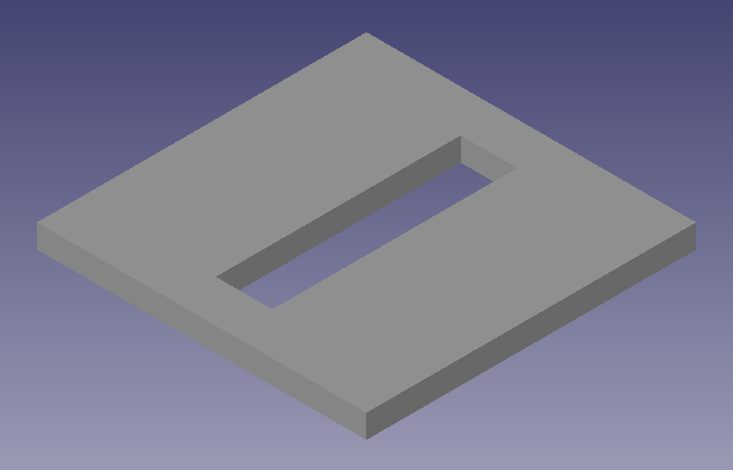
\includegraphics[width = 2cm]{./images/ppt_F20.png}} \hspace{0.1cm}
\subfloat[S40\_40]{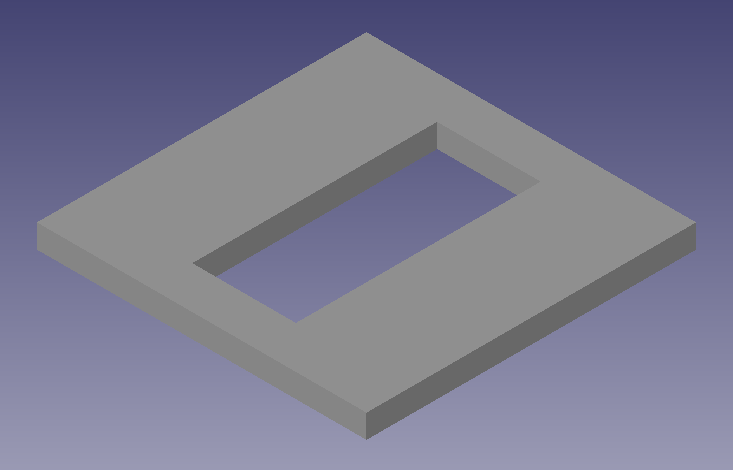
\includegraphics[width = 2cm]{./images/ppt_S40.png}} \hspace{0.1cm} 
\subfloat[M20\_100]{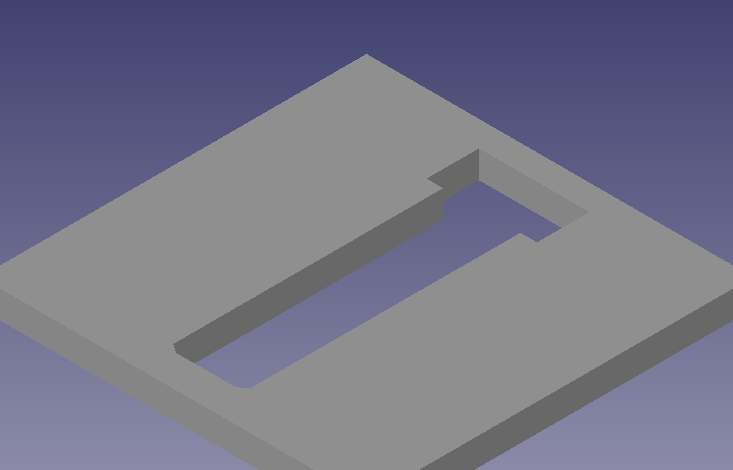
\includegraphics[width = 2cm]{./images/ppt_M20_100.png}}  \hspace{0.1cm}
\subfloat[M20]{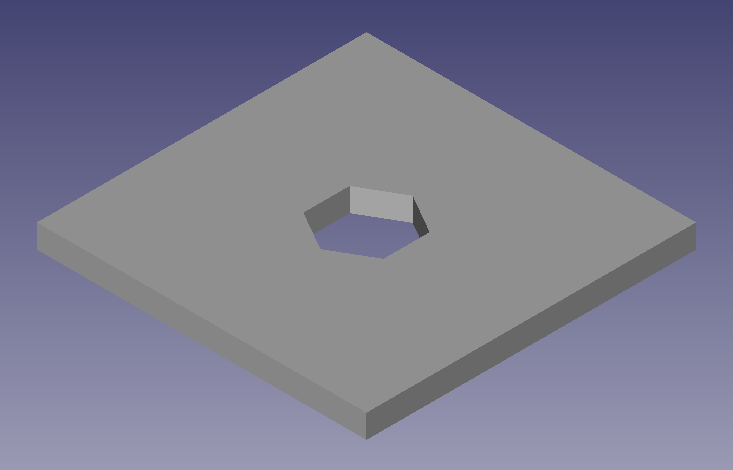
\includegraphics[width = 2cm]{./images/ppt_M20.png}}  \hspace{0.1cm}
\subfloat[M30]{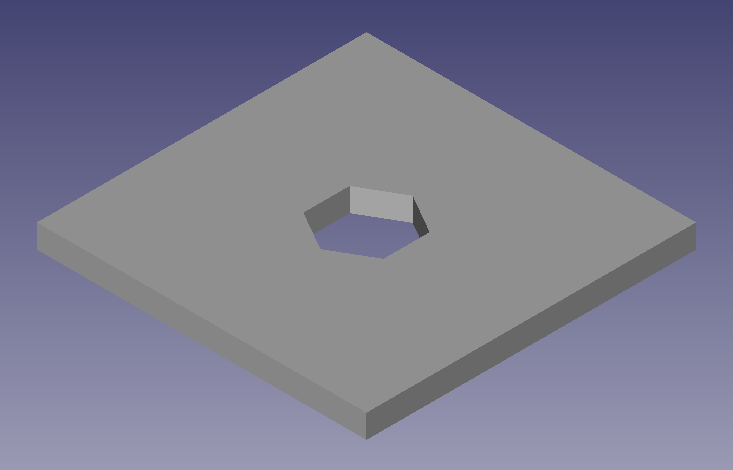
\includegraphics[width = 2cm]{./images/ppt_M30.png}}  \hspace{0.1cm}
\subfloat[R20]{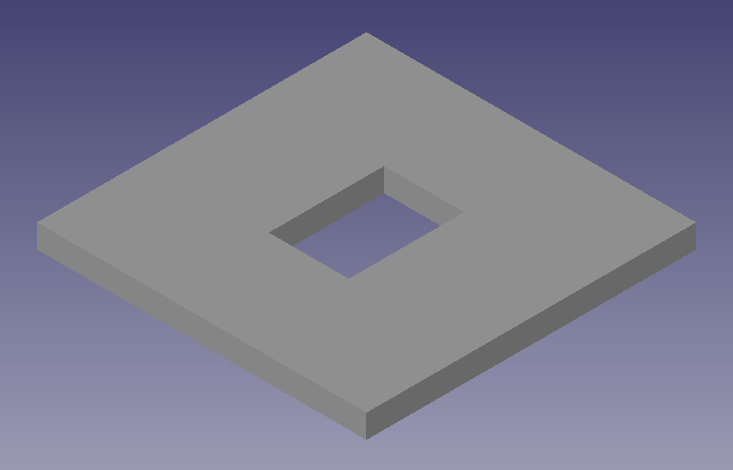
\includegraphics[width = 2cm]{./images/ppt_VR20.png}} \\
\subfloat[F20\_20]{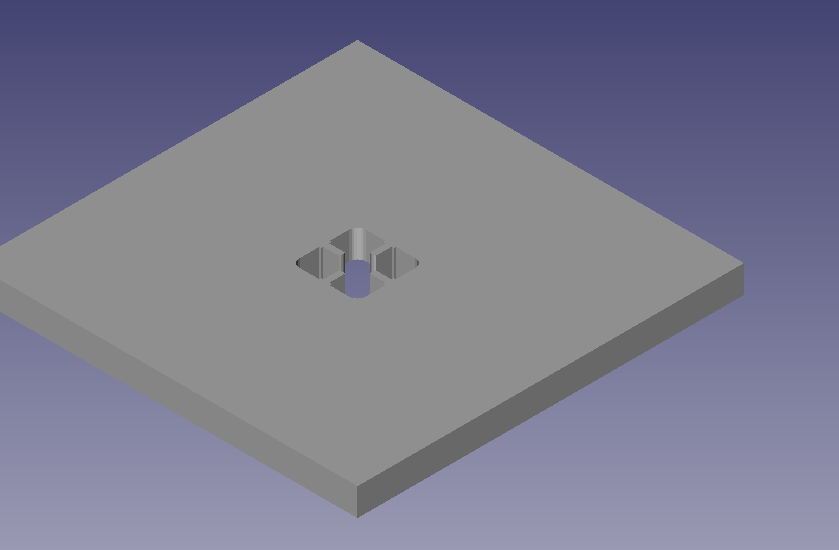
\includegraphics[width = 2cm]{./images/ppt_F20_v.png}}  \hspace{0.1cm}
\subfloat[S40\_40]{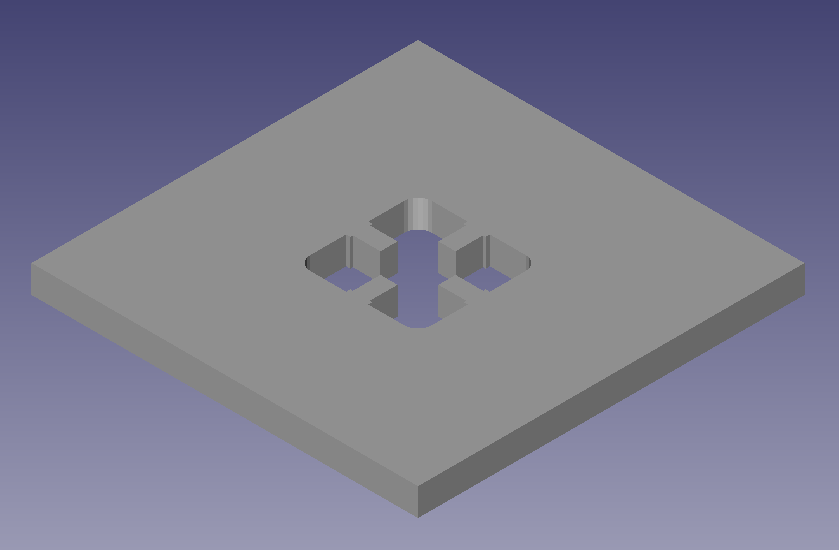
\includegraphics[width = 2cm]{./images/ppt_S40_v.png}}   \hspace{0.1cm}
\subfloat[M20\_100]{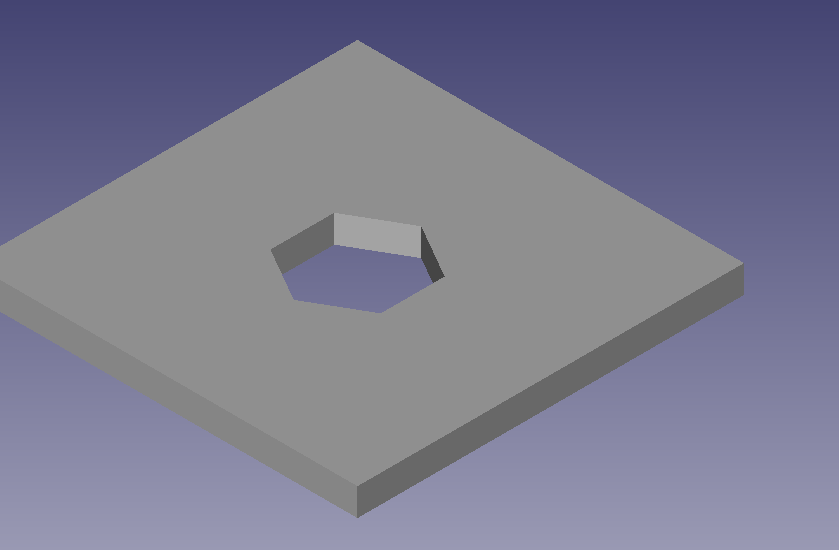
\includegraphics[width = 2cm]{./images/ppt_M20_100_v.png}} \hspace{0.1cm}
\subfloat[M20]{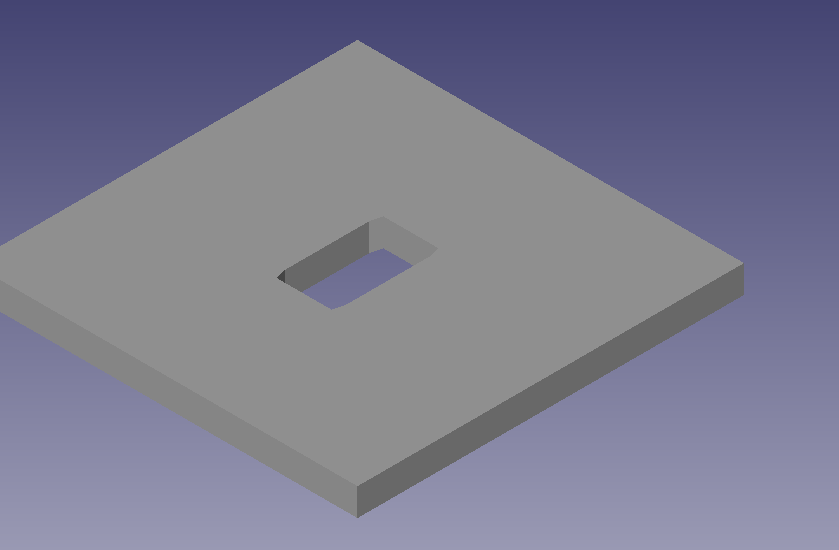
\includegraphics[width = 2cm]{./images/ppt_M20_v.png}}  \hspace{0.1cm}
\subfloat[M30]{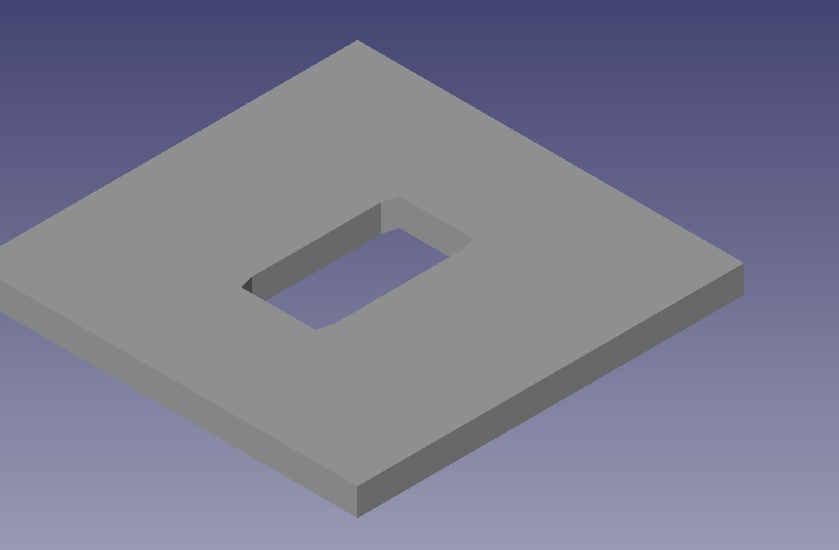
\includegraphics[width = 2cm]{./images/ppt_M30_v.png}}  \hspace{0.1cm}
\subfloat[R20]{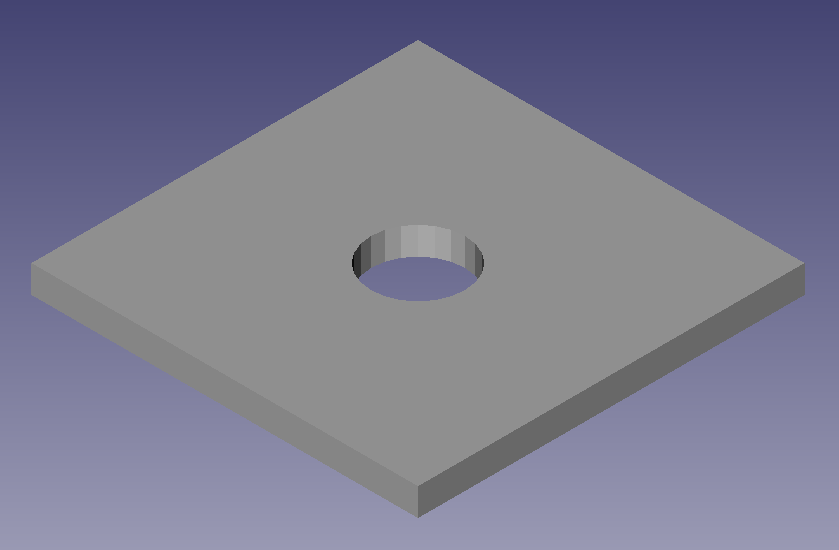
\includegraphics[width = 2cm]{./images/ppt_VR20_v.png}} 
\end{center}
\caption{Illustration of horizontal (top row) and vertical (bottom row) cavities for the different kind of manipulation objects.}
\label{fig:ppt_tiles}
\end{figure}


\paragraph{Manipulation Objects}
The manipulation objects used in this test are defined by the instances described in Table~\ref{tab:Instances}.

\paragraph{Task}
The objective of the task is to pick the objects which are placed on one service area and make a precise placement in the corresponding cavity at the service area with the special PPT platform (an example configuration is illustrated in Figure \ref{fig:ppt_plattform}). 

\begin{figure}
\centering
\includegraphics[width=0.6\textwidth ]{./images/ppt_plattform.jpg}
\caption{The PPT platform including five cavity tiles}
\label{fig:ppt_plattform}
\end{figure}

The task consists of multiple grasp and place operations, possibly with base movement in between, which will, however, be short. Note that the placement of the object in the cavity is finished when the object is fallen into the cavity (i.e. at least some part of the object has to touch ground floor underneath the cavity).

%
%\subsection{Complexity Levels}
%
%All Complexity Options from BMT apply.
%
%\subsubsection{PPT Orientation Complexity (bonus factor = 0.2):}
%The cavities can be placed in all orientations.
%\subsubsection{PPT Rotation Complexity (bonus factor = 0.2):}
%The cavities can be placed in all orientations.

\paragraph{Rules}
The following rules have to be obeyed:

\begin{itemize}

\item A single robot is used.
\item The robot has to start from outside the arena and to end in the final.
\item The order in which the teams have to perform will be determined by a draw.
\item The robot will get the task specification from the referee box.
\item A service area counts as successfully reached as defined in Section~\ref{ssec:Navigating}.
%\item A manipulation object counts as successfully grasped as specified in Section~\ref{ssec:GraspingObjects}.
\item An object counts as placed correctly if it fell through the correct cavity and touches the ground beneath. It may happen that an object blocks the cavity for the next object, e.g. by standing upright on the floor. In that case a referee may remove that object (which remains to count as a successful place). If the referee is not able to do so and the robot places another object into the blocked cavity, it counts as a correct placement if it would have been successful without the blocking object.
\item The run is over when the robot reached the final position or the designated time has expired.
\item The score for this test will be calculated as defined in \ref{sec:ScoringAndRanking}.

\end{itemize}

%\subsection{Scoring}
%Points are awarded as follows:
%
%\begin{itemize}
%\item 50 points are awarded for successfully grasping an object.
%\item 100 points are awarded for successfully placing a manipulation object into the correct cavity.
%\item 50 points are awarded if the task specification has been completely fulfilled. The task is considered as fulfilled if all objects have been dropped in the right cavity. The robot does not have to leave the arena.
%\item a penalty of -50 points is given for each object which has been dropped into the wrong cavity
%\item The reached points of a test will be multiplied with a defined complexity factor depending on the previously chosen complexity level.
%\end{itemize}




% !TEX root = ../Rulebook.tex
%\newpage
\section{Rotating Table Test}
\label{sec:Rotating Table Test}

The \iaterm{Rotating Table Test}{RTT} introduces moving objects to the competition.
A total of six objects are placed on the rotating table (\Marco{add ref to arena design, special rtt}), of which three must be picked and three are decoy objects.

This requires robots to detect objects and estimate their trajectory in order to grasp them successfully.
To lower the difficulty of this task, the table continously spins with a constant speed, enabling robots to use data from multiple rotations to calculate the optimal grasping position and move their manipulator in time.

It is explicitly NOT allowed to stop the table (e.g. by pushing the gripper into the table surface).
It is also explicitly NOT allowed to position the gripper in a way that blocks the objects 
unless it is during the grasping process of a target object and does not affect the table rotation or other objects.

The table starts spinning once the runtime of each team has started.
The initial table rotation is the same for each team to ensure comparability.  

As navigation is not the focus of this test, robots only have to travel to the rotating table and do not have to move to the FINISH location. The run ends once all three objects have been picked or a rule violation has been called by the referees.



%
%\paragraph{Purpose and Focus of the Test}
%The purpose of the \iaterm{Rotating Table Test}{RTT} is to assess the robot's ability to manipulate moving objects which are placed on a rotating turntable. The test demands fast perception and manipulation skills in order to pick up objects from a moving surface.
%
%\paragraph{Scenario Environment}
%The same arena as for the Basic Manipulation Test is used. In case that the arena does not already include such a device (see Figure \ref{fig:conveyor_belt}), it will be added only for this particular test.
%
%\begin{figure} [h!]
%	\begin{center}
%%		\subfloat[Conveyor belt]{\includegraphics[height = 4cm]{./images/conveyor_belt.jpg}} 
%%		\hspace{1cm}
%		\includegraphics[height = 6cm]{./images/rotating_table.jpg}
%	\end{center}
%	\caption{Illustration of a rotating table used in the competition.}
%	\label{fig:conveyor_belt}
%\end{figure}
%
%
%
%\paragraph{Manipulation Objects}
%The manipulation objects used in this test are defined by the instances described in Table~\ref{tab:Instances}.
%
%\paragraph{Task}
%The task of the robot is to navigate to the location of the rotating table and to grasp all objects from the moving table. The objects can pass multiple times in front of the robot, until the maximum time for the run is over. The robot is supposed to place the grasped objects on the robot itself.
%
%
%%\subsection{Complexity Options}
%%All Complexity Options from BMT apply.
%
%
%%\subsubsection{Speed Complexity (pick one):}
%%
%%\begin{itemize}
%%\item low speed (bonus factor = +0.0): The conveyor belt speed will be not more than 0.5 cm/s
%%\item medium speed (bonus factor = +02):	The conveyor belt speed will be not more than 0.75 cm/s
%%\item high speed (bonus factor = +0.4): The conveyor belt speed will be not more than 0.10 cm/s
%%\end{itemize}
%
%
%
%\paragraph{Rules}
%The following rules have to be obeyed:
%
%\begin{itemize}
%\item A single robot is used.
%\item The robot has to start from outside the arena and to end in the final.
%\item The order in which the teams have to perform will be determined by a draw.
%\item The objects are placed on the rotating table before the run starts by the OC or TC.
%\item The speed of the rotating table is determined by the OC or TC just before the test starts.
%\item The robot will get the task specification from the referee box.
%\item A service area counts as successfully reached as defined in Section~\ref{ssec:Navigating}
%\item A manipulation object counts as successfully grasped as specified in Section~\ref{ssec:PlacingObjects}.
%\item The objects have to be grasped actively from the moving table. The robot is not allowed to stop the items with its gripper.
%\item The run is over when the robot reached the final position or the designated time has expired.
%\item The score for this test will be calculated as defined in \ref{sec:ScoringAndRanking}.
%\end{itemize}
%
%
%
%%
%%\subsection{Scoring}
%%Points are awarded as follows:
%%
%%\begin{itemize}
%%\item 200 points are awarded for successfully grasping an object from the conveyor belt 
%%\item -150 points are given if an object dropped onto the ground, is placed not on the robot itself or dropped from the end of the conveyor..
%%\item -100 points are given if the referees had to switch on the belt manually after signalled by a team member, while a working automatic wireless mechanism to switch it on was available.
%%\item 50 points are awarded if the task has been fully achieved (when all objects placed on the belt are grasped).
%%\end{itemize}


\section{Final}
\label{sec:Final}

The \iaterm{Final Run}{Final} acts as the full benchmark for robots, including all elements of \RCAW.
With the number of objects and active service areas at its peak, task planning and execution speed may become a limiting factor for competing robots. The following paragraph summarizes the final, but DOES NOT override the test specification in table \ref{fig:test_specifications_instance}.

\paragraph{Final}
\begin{itemize}
\item Ten randomly selected objects have to be transported.
\item Eight randomly selected decoy objects are placed onto one or more randomly selected (active) service areas
\item There will be eight active service areas (four tables,  two shelfs, one Rotating Table and one Precise Placement table)
\item All table heights are used (0-15 $\si{\centi\meter}$).
\item Two objects must be picked from a shelf (lower part).
\item Two objects must be picked from the Rotating Table.
\item Two objects must be placed on a shelf (top part).
\item Two objects must be placed in the Precision Placement Cavity.
\item Four objects must be placed into a container (two in blue, two in red).
\item Two visual and two physical obstacles are placed inside the arena (two blocking, one semi-blocking, one non-blocking).
\item Four service areas will have an arbitrary surface.
\end{itemize}

% !TEX root = ../Rulebook.tex
\section{Test Specification Summary}
\renewcommand{\arraystretch}{1.1}
\newcommand{\R}[2]{
	\begin{turn}{90}
		\begin{minipage}[][1em][c]{#2}
		#1
	  \end{minipage}
	\end{turn}
}
\newcommand{\cir}[1]{\hspace{0.5em}\unitlength1ex\begin{picture}(2.8,2.8)%
\put(0.75,0.75){\circle{2.8}}\put(0.75,0.75){\makebox(0,0){#1}}\end{picture}}
\newcommand{\Y}{\tiny \CIRCLE}
\newcolumntype{P}[1]{>{\centering\arraybackslash}p{#1}}

\definecolor{headlineColor}{rgb}{.7,.7,.7}
\definecolor{sectionColor}{rgb}{.7,.1,.1}

\newcommand{\C}{\cellcolor{sectionColor}}
%\begin{landscape}
%\begin{table}[h!]
% \centering
% \begin{tabular}{|l|l|l*{11}{|P{1cm}}|}
%   \hhline{~~~--------}
%   \multicolumn{3}{l|}{ }                   &  \multicolumn{8}{c|}{Instances}                        \\
%   \hhline{~~~--------}
%   \multicolumn{3}{l|}{ }                   &\cir{1}&\cir{2}&\cir{3}&\cir{4}&\cir{5}&\cir{6}&\cir{7} \\
%   \multicolumn{3}{r|}{ }                   & BMT   & BTT1  & BTT2  &  BTT3 &  PPT  &  RTT  & Final  \\
%   \hhline{~~~--------} \hline
%   \multirow{5}{0.5cm}{\R{\centering Objects}{3.0cm}}
%   & \RCAW \&  RoCKIn            & atwork-commander   & 5     & 5     & 6     & 6     & 3      & 3     & 10    \\ \hhline{~----------}
%   & Decoy                       & TC   &       & 3     & 3     & 3     &        & 3     & 5     \\ \hhline{~----------}
%	 & Position                    &          & Ref   & Ref   & Ref   & Ref   & Team   & Ref   & Ref   \\ \hhline{~----------}
%	 & Rotation                    &          & Team  & Ref   & Ref   & Ref   & Team   & Team  & Ref   \\ \hhline{~----------}
%	 & Orientation                 &          & Team  & Team  & Team  & Ref   & Team   & Team  & Ref   \\ \hline
%   \multirow{6}{0.5cm}{\R{\centering Service area}{3.5cm}}
%   & Estimated Active            & atwork-commander   & 2     & 3     & 4     & 5     & 2      & 1     & 8     \\ \hline
%   & Table height                & atwork-commander   &       &       & 0 cm  &       &        &       &  0 cm \\
%   &                             &          &       &       & 5 cm  &       &        &       &  5 cm \\
%   &                             &          & 10 cm & 10 cm & 10 cm & 10 cm &  10 cm & 10 cm & 10 cm \\
%   &                             &          &       &       & 15 cm &       &        &       & 15 cm \\ \hhline{~----------}
%	 & Arbitrary surface           & TC   &       & 1     & 2     & 2     &        &       & 3     \\ \hline
%	 \multirow{3}{0.5cm}{\R{\centering Arena }{1.5cm}}
%	 & Physical Obstacles          & TC  &       &       & 2     & 2     &        &       & 2     \\ \hhline{~----------}
%	 & Virtual Obstacles           & TC  &       & 2     &       & 1     &        &       & 2     \\ \hhline{~----------}
%   &                             &          &       &       &       &       &        &       &       \\ \hhline{-----------}
%   \multirow{3}{0.5cm}{\R{\centering Grasping }{1.64cm}}
%   & Shelf unit                  & atwork-commander   &       &       &       & 2     &        &       & 2     \\ \hhline{~----------}
%	 & Rotating table          & Referee  &       &       &       &       &        & 3     & 1     \\ \hhline{~----------}
%   & Rotating direction          &          &       &       &       &       &        & Team  & Ref   \\ \hline
%   \multirow{8}{0.5cm}{\R{\centering Placement}{2.5cm}}
%   & Preisicon placement table  & atwork-commander   &       &       &       &       & 3      &       & 1     \\ \hhline{~----------}
%   & Shelf unit                  & atwork-commander   &       &       &       & 1     &        &       & 1     \\ \hhline{~----------}
%   & Red container               & atwork-commander   &       &       &       & 2     &        &       & 2     \\ \hhline{~----------}
%   & Blue container              & atwork-commander   &       &       &       & 2     &        &       & 2     \\ \hhline{~----------}
%   & Rotating turntable          & atwork-commander   &       &       & 1     &       &        &       &       \\ \hhline{~----------}
%   & Cavities Position           &    &       &       &       &       & Ref	   &       & Ref   \\ \hhline{~----------}
%   & Cavities Rotation	         &  &       &       &       &       & Ref    &       & Ref   \\ \hhline{~----------}
%   & Cavities Orientation	       &   &       &       &       &       & Team   &       & Team  \\ \hline \hline
%   \multicolumn{2}{|l|}{Duration}
%                                 & atwork-commander   & 5min  & 6min  & 10min & 10min & 4min   & 4min  & 13min \\
% 		\hline
% \end{tabular}
% \caption{Test specification in the instances of the \RCAW \YEAR competition.}
% \label{tab:Instances}
%\end{table}


\begin{figure}[h!]
	\centering
	\includegraphics[width= 1.0\textwidth ]{./images/tabels/robocup_env.png}
	\caption{Test specification in the environment of the \RCAW \YEAR competition.}
	\label{fig:test_specifications_environment}
\end{figure}

\begin{figure}[h!]
	\centering
	\includegraphics[width= 1.0\textwidth ]{./images/tabels/robocup_instance.jpg}
	\caption{Test specification in the instances of the \RCAW \YEAR competition.}
	\label{fig:test_specifications_instance}
\end{figure}
%\end{landscape}





%\newpage
%\section{Test Variability} \label{sec:TestVariability}

%The different optional parameters and configurations for each task are 
%mentioned in Section~\ref{sec:ArenaDesign} and \ref{sec:ManipulationTasks}. 
%Figure~\ref{fig:complexityTree} summarizes the possible variations and 
%emphasizes aspects that may be chosen.

%\begin{figure}[ht]
%\centering
%\tikzset{
  basic/.style  = {draw, rectangle, thin, text width=2cm, 
	                 rounded corners=2pt, align=center},
  root/.style   =  {basic},
  level 2/.style = {basic, sibling distance=45mm},
  level 3/.style = {basic, align=left},
  level 4/.style = {basic, align=left, fill = white!50, node distance = 0.7cm},
	box/.style = {draw, black, dashed}
}

\begin{tikzpicture}[
  font = \footnotesize,
  level 1/.style={sibling distance=70mm},
  edge from parent/.style={->,draw},
  >=latex]

% root of the the initial tree, level 1
\node[root] {Complexities}
% The first level, as children of the initial tree
  child {node[level 2] (c1) {Manipulation}
       child  {node[level 3]  (OBJECTS) {Objects}}
       child {node[level 3]  (GRASPING) {Grasping} }
       child {node[level 3, xshift =-2cm]  (PUTTING) {Putting down} }
	}
  child {node[level 2, xshift=-1cm] (ARENA) {Arena}};

%% OBJECTS
\begin{scope}[every node/.style={level 4,  top color=white!50,bottom color=gray!50,shading angle=45}]
\node [below of = OBJECTS, xshift=15pt, yshift=-20pt] (c11) {@work};
\node [below of = c11] (c12) {Rockin};
\node [below of = c12] (c13) {arbitary};
\node [below of = c13, yshift=-5pt] (c14) {number};
\end{scope}

\node [box, fit = (c11) (c12) (c13)] (BOX) {};
\node at (BOX.north west) [anchor = south west] {Type};

%% GRASPING
\begin{scope}[every node/.style={level 4}]
\node [below of = GRASPING, xshift=28pt, yshift=-20pt] (c21) {0cm};
\node [below of = c21] (c22) {10cm};
\node [below of = c22] (c23) { ??cm};
\node [below of = c23] (c24) { ??cm};
\node [below of = c24, top color=white!50,bottom color=gray!50,shading angle=45, yshift=-18pt] (c25) {Position};
\node [below of = c25, top color=white!50,bottom color=gray!50,shading angle=45] (c26) {Rotation};
\node [below of = c26, top color=white!50,bottom color=gray!50,shading angle=45] (c27) {Orientation};
\node [below of = c27, yshift=-18pt,] (c28) {red};
\node [below of = c28] (c29) { blue};
\end{scope}

\node [box, fit = (c21) (c22) (c23) (c24)] (BOX) {};
\node at (BOX.north west) [anchor = south west] {Height};

\node [box, fit = (c25) (c26) (c27)] (BOX) {};
\node at (BOX.north west) [anchor = south west] {Object Pose};

\node [box, fit = (c28) (c29)] (BOX) {};
\node at (BOX.north west) [anchor = south west] {Container};

%% ARENA
\begin{scope}[every node/.style={level 4}]
\node [below of = ARENA, xshift=15pt, yshift=-20pt] (c31) {Static};
\node [below of = c31] (c32) {Dynamic};
\node [below of = c32, yshift=-5pt] (c33) {Barrier tape};
\end{scope}

\node [box, fit = (c31) (c32)] (BOX) {};
\node at (BOX.north west) [anchor = south west] {Obstacles};

% lines from each level 1 node to every one of its "children"
 \foreach \value in {1,2,3,4}
   \draw[->] (OBJECTS.195) |- (c1\value.west);

 \foreach \value in {1,...,9}
   \draw[->] (GRASPING.195) |- (c2\value.west);
	
 \foreach \value in {1,...,4}
   \draw[->] (PUTTING.345) |- (c2\value.east);

 \foreach \value in {8,...,9}
   \draw[->] (PUTTING.345) |- (c2\value.east);
	
\foreach \value in {1,2,3}
   \draw[->] (ARENA.195) |- (c3\value.west);

\end{tikzpicture}

%\caption{Aspects of variability that may be integrated in a specific instance of a test.}
%\label{fig:complexityTree}
%\end{figure}



\chapter{Scoring and Ranking}
% !TEX root = ../Rulebook.tex
\section{Scoring} \label{sec:ScoringAndRanking}

For each test the calculation of scores is defined individually, comprising points for achieving certain subtasks, points for winning a run and penalty points.
\par
Each test provides a set of so-called feature variations encoding the overall variability of the test (e.g. whether obstacles can occur or not, number and type of manipulation objects). To enhance comparability among different test runs, all teams will have to perform the same test instances as specified in Table~\ref{tab:Instances}.
\par
If not specified otherwise, the following set of scoring rules applies for each test:


Explanation of the terms:
\begin{itemize}
\item Correct navigating is defined in Section \ref{ssec:Navigating}
\item Correct grasping is defined in Section \ref{ssec:GraspingObjects}
\item Correct placing is defined in Section \ref{ssec:PlacingObjects}
\end{itemize}

\section{Simplifications}
Teams may use simplifications, which will result in a reduction of scores for the given run:

\begin{itemize}
	\item Use of external sensors: \hfill -200 points
	\item Use of other external objects (e.g. to support localization): \hfill -100 points
	\item Use of own loading or unloading areas: \hfill -200 points
\end{itemize}

Additional simplifications are specified for individual tests. These reductions do not count as penalty points. Teams that want to make use of the simplifications above have to announce them in advance of the competition to the TC. The TC might forbid the use of specific elements for simplification if these are not in the spirit of the league or may cause disproportionate advantages for a team.

\section{Perfect Runs}
All teams fully complete a perfect run will receive a completion bonus of 0.75 points per second left on the run time. These points are only awarded if the run is perfect, i.e. all objectives reached without any penalties.

\section{Penalties}
\label{sec:penalties}
Penalty points are given as follows, each time again the incident occurs:

\begin{itemize}
	\item A manipulation object is lost or placed anywhere outside of a service areas: \hfill -100 points
	\item Delivering a wrong manipulation object to service area \hfill -50 points
	\item Minor collision (see Section \ref{sec:Collisions}): \hfill -50 points
	\item Major collision (see Section \ref{sec:Collisions}): \hfill -50 points and termination of the run
\end{itemize}

\section{Collisions}\label{sec:Collisions}
For reasons of safety of people and property it is strictly unwanted for the robot to collide with any of the environmental objects. Only collisions of the manipulator with the upside of the service area are allowed. The different kind of collisions that can occur are defined in the following subsections.

\subsection{Minor Collision}
If the robot collides with the environment, but does not move the environment and the wheels are not spinning, it is considered a minor collision.

\subsection{Major Collision}
If the robot collides with the environment and moves it or its wheels are spinning, it is considered a major collision.

\subsection{Barrier Tape collision}
If any part of the robot touches a barrier tape, it is considered a barrier tape collision. The maximum penalty resulting from these collisions depends on the specific competition instance and is listed in Tab.~\ref{tab:InstancePoints}.

Touching or passing a Barrier Tape when entering or exiting the arena does not count as collision.


%Some tests have three so-called complexity levels. A complexity level (low, medium and high) encodes the difficulty of the test such as the number of objects to manipulate or whether the arena is equipped with obstacles or without.

%Every team decides for each run of a test in which complexity level they want to participate. This decision must be made by all teams when asked for by the OC, but at least before the first team starts a particular run.



\section{Restarts}
Teams might use one so-called restart in a run. Restarts have the following aspects:

\begin{itemize}

	\item Per run, at most one restart is allowed for a team, if not specified otherwise in a test.
	\item At any time during a run, the team can call for a restart to the referees.
	\item When the referees acknowledge the call for restart, the team may enter the arena. The time will continue running.
	\item The arena and the robot will be reset exactly to the setup at the beginning of the run (except the timer for the run). Random elements such as obstacles or object positions remain like before.
	\item The points for this run achieved so far are reset to zero.
	\item Scores that are received after a restart are multiplied by a factor of 0.75.
	\item The referees decide when the arena is prepared again for the restart. If the robot is not yet ready, teams can keep trying to get it ready until the time for the run is over.
	\item As soon as the team signals that the robot is ready, the task specification is sent again.
	\item Afterwards the start signal is sent from the referee box.

\end{itemize}


\section{Ranking}
The tests will occur in the instances shown in Table~\ref{tab:Instances}. Ranking of the teams will be based on the sum of the achieved points over all the tests.

A team cannot get less than zero points for one run.
The scores of the tests of the first stage are summed up, and the teams with the highest sums proceed to the next stage.

In case of a tie, the OC will either schedule a deciding run or continue with a higher number of participants.

\all{We should change the test durations here.}
\christoph{Please check the new scoring - I changed the following entries: Grasping from RTT: 300, lower shelf: 300, upper shelf: 150
Placing to PPT: 200, lower shelf: 150}

%\setlength{\tabcolsep}{4.75pt}
\renewcommand{\arraystretch}{1.1}
\newcommand{\R}[2]{
	\begin{turn}{90}
		\begin{minipage}[][1em][c]{#2}
		#1
	  \end{minipage}
	\end{turn}
}

\newcommand{\cir}[1]{\hspace{0.5em}\unitlength1ex\begin{picture}(2.8,2.8)%
\put(0.75,0.75){\circle{2.8}}\put(0.75,0.75){\makebox(0,0){#1}}\end{picture}}
\newcommand{\Y}{\tiny \CIRCLE}
\newcolumntype{P}[1]{>{\centering\arraybackslash}p{#1}}

\definecolor{headlineColor}{rgb}{.7,.7,.7}
\definecolor{sectionColor}{rgb}{.7,.1,.1}

\newcommand{\C}{\cellcolor{sectionColor}}

\begin{landscape}
\begin{table}[h!]
 \centering
 \begin{tabular}{|l|l|l*{12}{|P{1cm}}|}
   \hhline{~~~--------}
   \multicolumn{3}{l|}{ } &  \multicolumn{8}{c|}{ Instances}\\
   \hhline{~~~--------}
   \multicolumn{3}{l|}{ }          &\cir{1}&\cir{2}&\cir{3}&\cir{4}&\cir{5}&\cir{6}&\cir{7}&\cir{8}\\
   \multicolumn{3}{r|}{     }        & BNT   & BMT   & BTT1  & BTT2  &  BTT3 &  PPT  &  RTT & Final\\
   \hhline{~~~--------} \hline
     \multirow{5}{0.5cm}{\R{\centering Objects}{3.0cm}}
     &  \RCAW \&  RoCKIn    & RefBox   &       &   5   &  5     &   6   &  6   &   3    &  3  & 10 \\ \hhline{~----------}
     &  Decoy               & RefBox   &       &       &  3    &   3     &   3   &       &   3     & 5   \\ \hhline{~----------}
		 &  Position            &          &       &   Ref  &   Ref  &  Ref  &  Ref   &   Team  &  Ref & Ref  \\ \hhline{~----------}
		 &  Rotation         &          &       &  Team &   Ref   &  Ref    &  Ref    &   Team  & Team& Ref   \\ \hhline{~----------}
		 &  Orientation      &          &       &  Team &   Team  &  Team   &  Ref   &  Team  &Team &  Ref  \\ \hline
     \multirow{5}{0.5cm}{\R{\centering Service area}{2.4cm}}
		 &  Table height    & RefBox   &       & 10 cm & 10 cm &  0 cm\newline 5 cm \newline 10 cm\newline 15 cm   & 10 cm  &  10 cm &    10 cm & 0 cm\newline 5 cm\newline 10 cm\newline 15 cm \\ \hhline{~----------}
		 & Arbitrary surface & RefBox &       &       &   1     &   2   &  2   &        &    &  3  \\ \hline
		 \multirow{3}{0.5cm}{\R{\centering Arena }{1.5cm}}
	   & Obstacles (static) & Referee &   2   &       &       &   2   &   2   &       &   & 2   \\ \hhline{~----------}
		 & Barrier tape       & Referee &   2   &       &    2   &       &   1   &       &   & 2   \\ \hhline{~----------}
		 & Waypoints          & RefBox  &   9   &       &       &       &       &       &   &    \\ \hline
    \multirow{3}{0.5cm}{\R{\centering Grasping }{1.7cm}}
     & Shelf unit        & RefBox   &       &       &       &       &   2   &       &    & 2   \\ \hhline{~----------}
		 & Rotating turntable& Referee  &      &       &       &       &       &        & 3  & 1   \\ \hhline{~----------}
     & Rotating direction&          &      &       &       &       &       &        & Team & Ref   \\ \hline
     \multirow{8}{0.5cm}{\R{\centering Placement}{2.5cm}}
     & Cavity platform with decoy& RefBox   &       &       &       &       &       &  3   &   & 1   \\ \hhline{~----------}
     & Shelf unit          & RefBox &       &       &       &       &   1     &        &   & 1   \\ \hhline{~----------}
     & Red container       & RefBox &       &       &       &       &  2   &       &   &  2   \\ \hhline{~----------}
     & Blue container      & RefBox &       &       &       &       &  2   &       &   &  2   \\ \hhline{~----------}
     & Rotating turntable  & RefBox &       &       &       &   1   &      &       &   &    \\ \hhline{~----------}
     & Cavities Position     & RefBox &       &       &       &      &      &   Ref	  &   &  Ref   \\ \hhline{~----------}
     & Cavities Rotation	& RefBox &       &       &       &      &      &   Ref    &   &  Ref   \\ \hhline{~----------}
     & Cavities Orientation	& RefBox &       &       &       &      &      &   Team   &   &  Team  \\ \hline \hline
  	\multicolumn{2}{|l|}{Duration}
    & RefBox & 5 min & 5 min & 5 min  &   8 min &   8 min &  4 min &  4 min & 10min \\
 		\hline
 \end{tabular}
 \caption{Test specification in the instances of the \RCAW \YEAR competition.}
 \label{tab:Instances}
\end{table}
\end{landscape}

\begin{landscape}
\begin{table}
 \centering
 \begin{tabular}{|p{5.5cm}*{9}{|P{1cm}}|}
   \hhline{~--------}
   \multicolumn{1}{l|}{ } &  \multicolumn{8}{c|}{ Instances}\\
   \hhline{~--------}
   \multicolumn{1}{l|}{ }          &\cir{1}&\cir{2}&\cir{3}&\cir{4}&\cir{5}  &\cir{6}&\cir{7}&\cir{8}\\
   \multicolumn{1}{r|}{     }       & BNT   & BMT   & BTT1  & BTT2  &  BTT3 & PPT   &  RTT & Final\\
   \hhline{~--------}
   \hline
    Correct destination reached     &  50  &      &       &       &       &       &       &      \\
		  \hspace{0.5cm} correct service area reached&     &   25   &  25     &   25    &  25     &  25    &  25    &  25   \\ \hline
    Correct object grasping standard&      &  100   &  100    &  100     &  100    &       &       &   100  \\
		\hspace{0.5cm} round table        &      &      &       &       &       &       &   300       &   200   \\
		\hspace{0.5cm} PPT area           &      &      &       &       &       &  200  &       &   200  \\
		\hspace{0.5cm} arbitrary surface  &      &      &       &       &  150 ? &       &       &   150 ?  \\
		\hspace{0.5cm} shelf upper level  &      &      &       &       &  150  &       &       &   150  \\
		\hspace{0.5cm} shelf lower level  &      &      &       &       &  300  &       &       &  300  \\ \hline
    Correct object placing standard   &      & 75   & 75    & 75    &  75   &       &       &  75  \\
		\hspace{0.5cm} PPT area           &      &      &       &       &       &  200  &       &   200  \\
		\hspace{0.5cm} shelf upper level  &      &      &       &       & 150   &       &       &   150  \\
		\hspace{0.5cm} shelf lower level  &      &      &       &       &  150  &       &       &  150  \\ \hline
    Incorrect object placing        &      & -100 & -100  & -100  & -100  & -100  &       & -100  \\
    Incorrect object grasping       &      &      & -100  & -100  & -100  &       & -100  & -100  \\
    Completing whole task           &  50  &  75  &   100  &   100   &   250  &    50    &   75   &  300   \\ \hline\hline
    Maximum barrier \newline tape penalty    &  100  &      &  200  &       &  300  &       &       &  400  \\ \hline\hline
    Maximum attainable points\newline (time bonus not included)
	                                  & 500  &  1000 &  1050 &  1300  &  1400  &  850  &  700  &  2300 \\ \hline
 \end{tabular}
 \caption{Scoring in the instances of the \RCAW \YEAR competition.}
  \label{tab:InstancePoints}
\end{table}
\end{landscape}


\chapter{Virtual RoboCup}
\label{cha: VRC}
% !TEX root = ../Rulebook.tex

\section{General} 
\label{sec:VRCGeneral}

Due to the Covid-19 pandemic, the RoboCup 2021 will be held online. 
Therefore, paricipating teams must provide some infrastructure to enable the TC and OC to evaluate their performance.
This is new for everyone and requires extended communication, which is why every team should join the official discord server:

\href{Official Discort Server}{https://discord.gg/z6Yn6UvhxU}
Please participate in discussions and ask questions if you have any.

\section{Arena Setup} 
\label{sec:VRCArenaSetup}

As all teams will have different laboratory setups and some may not have the same resources (open space, workstations, etc. ) as others, no fixed arena design will be used for the Robocup@work 2021. We expect that this would either exclude some teams from the competitions or limit others in their test scenario design, which is why every team can design their own arena.

However, to ensure that the different robot performances can be compared using the existing scoring system (\ref{tab:Instances}), some rules are defined to encourage teams to create challenging arena designs. In addition to the basic rules described in \ref{sec:ArenaDesign}, teams are required to consider: 
  
\begin{itemize}
\item Arena size must be atleast 4m x 2m
\item The table placements should force the robot to move around the arena (not all the tables are next to each other)
\item Workstations should be accessible via multiple paths, so one of them may be blocked with obstacles (\ref{fig:vrc_arena_example} orange dots). Some space must be available for non-blocking obstacles (\ref{fig:vrc_arena_example} dark green dots).
\item Tables with the heights defined in (\ref{tab:Instances}) have to be provided (margin = 2cm). If a team doesn't have enough workstations of one type for a test, the TC may allow alternative table heights to be used (especially BTT3 and Final). This rule does not apply for the conveyor belt, the shelf and the precise placement station.
\item PPT cavities (a)-(f) (see \ref{fig:ppt_tiles}) must be provided. Teams may 3D print the cavities using the files in the leagues github. Standing objects are excluded. It must be possible to place ${N\_PLACE + 2}$ next to each other, so that atleast two decoy cavities can be used. 
\item Required arbitrary surfaces types: artificial grass, pvc floor / wood, mirror / aluminum foil, (plexi-)glass. 
These can be found in your local homedepot. (See fig. \ref{fig:vrc_obst_arbi}(b))
\item One path blocking and one small obstacle must be available both for physical objects and barriertape. (See fig. \ref{fig:vrc_obst_arbi}(a))
\end{itemize}

Figure~\ref{fig:vrc_arena_example} shows one possible example of an arena configuration in a small area.
Table heights are measured in cm. 
The orange dots mark possible path blockades, while the dark green lines mark optional obstacle placements. 


\begin{figure}[h!]
\centering
\includegraphics[width=0.9\textwidth ]{./images/vrc_arena_example.png}
\caption{Example Arena for a small VRC Setup --- Left: Annotated map - Right: Real Image }
\label{fig:vrc_arena_example}
\end{figure}

\begin{figure} [h!]
\begin{center}
\subfloat[Obstacle Placements]{\includegraphics[height = 5cm]{./images/vrc_obstacles.jpg}} \hspace{1cm}
\subfloat[Arbitrary Surfaces]{\includegraphics[height = 5cm]{./images/vrc_arbitrarys.jpg}}
\end{center}
\caption{Example obstacle placements and arbitrary surfaces}
\label{fig:vrc_obst_arbi}
\end{figure}


To enable the committee to generate fair tasks for every team, teams must provide detailed information about their arena and object inventory \textbf{1 month} prior to the first competition day. A zip-folder containing the following data must be sent via our discord server:

\begin{itemize}
\item Atleast two images of the arena from different perspectives. If two cannot cover the whole arena, teams must provide as many as needed.
\item A map of the arena with workstations marked (name + height). Teams may use an RVIZ screenshot containing the grid (1m cell size) and the occupancy grid (your map), which may be annotated using e.g. gimp (see also \ref{fig:vrc_arena_example}).
\item A list of available workstations in their arena (height and amount).
\item Images of the available arbitrary surfaces
\item Images of the available barriertape and obstacles
\item A list of available objects and containers (amount)
\item Image of the objects and containers
\item Images of the robot (all sides)
\item Robot dimensions in meter
\item Which tests the team intends to participate in
\item atWork-commande launchfiles
\end{itemize}

The folder must be named VRC2021-info-TEAM-NAME and shall contain the subfolders ARENA, OBSTACLES, OBJECT, ROBOT, TESTS, REFBOX. 
File names must contain information about the data (e.g. Arena-Image-1) and must not have default names (e.g. IMG2012).

The TC will decide if the individual arenas qualify for the tests defined in \ref{tab:Instances}. 
The main requirements are already specified in \ref{sec:VRCArenaSetup}, while the table describes individual task requirements more precisely.
 
If an arena does not qualify, the TC must notify the team \textbf{3 weeks} before competition starts, 
briefing the team about shortcomings and possible solutions. 
The team then has \textbf{1 week} to follow the TCs advice and provide a new zip-folder.
If an arena does not qualify for a test, the TC may decide to exclude the associated team from those.
If an arena only partly qualifies (e.g. no barriertape available), score adjustments can be made.


\section{Camera Setup} 
\label{sec:VRCCameraSetup}

Since the referees are not present at the arena during the Virtual RoboCup, the arena and all activities of the robot must be shown via livestream. For this purpose, cameras must be able to monitor the entire arena for the referees and the cameras should be mounted at least at head height. No blind spots are allowed when streaming the arena, so that the referees can see and evaluate every activity of the robot. Furthermore, the PC used to start the runs should also be monitored with the cameras so that the referees can observe every interaction with the PC. One or more cameras can be used to stream the arena. The OC will announce the streaming software used and the maximum number of livestreams available before the competition.
\par
In addition to the cameras for the arena, there must be a person who follows the robot with a mobile camera and shows the robot's activities from close up. This allows the referees to detect even small mistakes. The person is allowed to enter the arena during the run. However, the person is not allowed to interact with the robot.
\par
A camera may also be attached to the robot to better show the robot's activities to the referees and spectators. The camera on the robot is optional.

\section{RoCKIn manipulation object set} 
\label{sec:VRCRoCKInSet}
The RoCKIn objects (see table \ref{tab:manipulation_objects_rockin}) are no longer produced and sold. Because of this, it is allowed to create these objects with a 3D printer at the Virtual RoboCup. However, the 3D printed RoCKIn objects must not be mixed with original objects. This means that the complete RoCKIn object set is either original or 3D printed. Furthermore, the 3D printed objects must have the same color. This applies only to the RoCKIn object set and not to the RoboCup@Work object set (see table \ref{tab:manipulation_objects}). The RoboCup@Work object set must not be 3D printed.


\section{Task Generation} 
\label{sec:VRCTaskGen}

The new atWork-commander implementation, which can be found here (https://github.com/robocup-at-work/atwork-commander), 
gives great opportunity to generate individual tasks for every participating team.

We advise all teams to use and test the new refbox. Teams must send configuration files for the new refbox with their arena design, so that the TC/OC can generate tasks for their arena. The config file for the arena shall contain the workstation names and heights and the available objects for a team. Teams may contact the committee via Discord if they face problems with this.  

As normally the atWork-commander would be provided by the OC onsite, no actual atWork-commander will be used during the online competition.
The OC will create the tasks for the tests using the official atWork-commander and the parameters provided by the teams. 
For each test, a single bagfile (10s) will be recorded which contains all topics published by the atwork\_commander.

Teams must be able to play a bagfile on an external computer, which is connected to the robot via WiFi.
The bagfile then must be played to start a competition. The robot should receive the task and start with the execution phase.

To prevent incompatible bagfiles during the competition, 
the OC will provide test bagfiles \textbf{2 weeks} before official competitions begin.
The working parameter and launchfiles will be saved and used to generate the specific task bagfiles for the competition.

\section{Competition Test Procedure} 
\label{sec:VRCTestExec}

\subsection{Preparation} 

Before a test begins, the OC will announce obstacle placements, object positions and arbitrary surface application to a team \textbf{10 minutes} prior to their timeslot. Teams must prepare the arena accordingly. The task bagfile will be sent out to the team \textbf{5 minutes} before their official timeslot. Note: The durations may be modified during the competitions if they show to be unsuitable.

\subsection{Test Start} 

The OC may count down before a competition (3, 2, 1, go), after which they start a timer according to the test durations in \ref{tab:Instances}. On GO command, the active team may access the keyboard of the remote pc \textbf{only} to start the bagfile. The cameraman/-woman must show that to the audience.

\subsection{Test Run} 

The audience and especially the refs watch the livestream and rate the performance. In case of a major collision or any other reason for a restart, the remote pc keyboard may be accessed to restart the robot and the bagfile. The replay of the bagfile command must be shown to the audience once again, and afterwards the keybord must not be used anymore.

\subsection{Test End} 

The run ends when the timer is up, with an optional margin of five seconds due to the possible network delay. The refs then gather and discuss their performance evaluation.  

\section{Scoring} 
\label{sec:VRCScoring}

The different arena setups make time bonuses unfair and will therefore not be given in the VRC 2021. 
The rest of the scoring will be the same as in a normal robocup scenario, with score/runtime adjustments and/or penalty points possible to compensate for missing test elements (see \ref{sec:VRCArenaSetup}). Such adjustments could be:

\begin{itemize}
\item The runtime for a test may be reduced if the arena is very small
\item If no barriertape is available, all penalty points for crossing will be applied
\item If no arbitrary surface is available, the object to pick will also be removed. 
\item No containers = no placement points given
\end{itemize}

Depending on the arena setups of all teams, these rules will be defined more precisely before the competitions begin.

\section{Technical Challenges} 
\label{sec:VRCTecCha}

The 2021 virtual robocup will focus on the main competition. No technical challenges will be performed during the official competitions this year. As some teams still requested technical challenges, we accept submissions for the cluttered pick test and the drawer test by video. This is because that we expect a relatively tight schedule due to the different time zones of the teams and we are unsure if the technical challenges may be performed otherwise.

As the challenges do not count into the official scoring, teams are allowed to modify their arena. They still must stick to the rules defined in \ref{cha: TCHA}. The bagfile for the specific challenge will be sent out to the teams on the first day of the competitions. Teams are required to record a video of their challenge with a camera setup similar to \ref{sec:VRCCameraSetup}, which must be cut in a way that it is possible to see every region of interest (robot, no operator on pc, arena) at all times. The video must be rendered to mp4 format and uploaded to a cloud (e.g. onedrive). 
Teams must provide a link to their video via our discord server with the deadline set to last competition day, more specificly the beginning of the final runs.

The committee will review all submissions and rate the individual performances with the help of the referee team after the finals have been completed. Videos that exceed the deadline will not be reviewed and the teams participation in the challenge will be cancelled.













\chapter{Technical Challenges} \label{cha:TechnicalChallenges}
\label{cha: TCHA}
% !TEX root = ../Rulebook.tex

In order to value very specific capabilities required in \RCAW technical challenges are part of \RCAW.
These challenges are designed to be included into the mayor competition after they have shown a potential as a benchmark in industrial robotics and have been at least solved in principal.
Each technical challenge is separately awarded. That means, teams can solely participate in the challenges without competing in the main competition.


% !TEX root = ../Rulebook.tex


\newpage
\section{Open Challenge}
During the Open Challenge teams are encouraged to demonstrate recent research results and the best of the robots’ abilities. It focuses on the demonstration of new approaches and applications to industrial tasks.

\subsection{Task}

The Open Challenge consists of a demonstration and an interview part. The performance of the teams is evaluated by a jury consisting of all team leaders, TC and OC members. Although it is supposed to be an open demonstration and the teams shall have freedom to develop their own ideas, a scientific and industrial tie will be considered in the jury's assessment. The topic of the demonstration should focus on one or multiple fields of the RoboCup@Work league namely robot manipulation, robot navigation and mapping, object detection and recognition.

\begin{itemize}
\item[1.] Setup and demonstration: The team has a maximum of 7 minutes for setup, presentation and demonstration.
\item[2.] Interview: After the demonstration, there is another 3 minutes where the team answers questions by the jury members.
\end{itemize}

\subsection{Presentation}
During the demonstration, the team can present the addressed problem and the demonstrated approach.
A video projector or screen, if available, may be used to present a brief (max. 1 minute) introduction to what will be shown. The team can also visualize robot’s internals, e.g., percepts.

\subsection{Jury​ ​evaluation}
Jury​:​ All teams have to provide one person (preferably the team-leader) to follow and evaluate the entire Open Challenge. A jury member is not allowed to evaluate and give points for the own team. The present members of the TC and OC will join the jury.  \par 
Evaluation:​ Both the demonstration of the robot(s), and the answers of the team in the interview part are evaluated. \par
For each of the following evaluation criteria, a maximum number of points (as defined by equation \ref{eq:criteriapoints}) is given per jury member:
\begin{itemize}
\item Overall demonstration
\item Robot autonomy in the demonstration
\item Realism and usefulness for industrial like applications (Can this be ported on real industrial scenarios?)
\item Novelty and (scientific) contribution
\item Difficulty and success of the demonstration
\end{itemize}

The maximum points for each criterion is calculated as:
\begin{equation}\label{eq:criteriapoints}
S_{c,max}=\frac{MaximumPointsForThisChallenge}{NumberOfEvaleuationCriteria}
\end{equation}
The maximum points for this challenge is 200 in \RCAW \YEAR .

Normalization​ ​and​ ​outliers:
\begin{itemize}
%\item The points given by each jury member are scaled to obtain a maximum point count as defined by equation \ref{}
\item The total score for each team is the mean of the jury member scores. To neglect outliers, the N best and worst scores are left out:
\end{itemize}

\begin{equation}\label{eq:totalpoints}
S=\frac{\Sigma TeamLeaderScore}{NumberOfTeams−(2N+1)}
\end{equation} 
$N = 2$ if $NumberOfTeams \geq 10$, $1$ if $NumberOfTeams < 10$. \par


%\subsection{Team-team​ ​interaction}
%There might be a team-team interaction component in the assessment of the open challenge in future years. 

%\subsection{Inter-league​ ​collaboration}
%There might be a inter-league collaboration component in the assessment of the open challenge in future years. 



%\chapter{Open Source Award}
%\section{Introduction and Motivation}

\todo{[Sebastian] From my perspective we should chancel the additional awards and challenges. The teams should concentrate on
the main competition.}

In order to foster the development of new teams and to increase cooperation among established teams, the league announces an Open Source Award. As demonstrated
in other \RC major leagues, releasing software and/or hardware as open source fosters the overall progress of the league. Similarly, to other open source awards in \RC, all institutions, persons and teams who took part in national and international \RCAW competitions in \YEAR or the previous year are eligible to participate. 

\section{Application}
The application should contain the following items: 

\begin{itemize}
	\item A technical report and description (max. 8 pages in Springer LNCS style) about the open source artifact (software/hardware or both). The report should briefly describe the open source project objectives, design decisions and most importantly should exemplify it's importance for the \RCAW competition and community.   
	\item A online reference, documentation, tutorial (e.g. website, Github page etc.) for the presented open source material. This includes also statements about licensing (e.g. which kind of open source license such as GPL, LGPL, Apache, etc.) and usage.  
\end{itemize}

Application deadline is the: 01.05.2016. Application material needs to be send via email to: \texttt{rc-work-tc@lists.robocup.org}. Please note, in case the evaluation committee receives  only applications which do not fulfill the desired level of quality, the award will not be given in \YEAR. The winner(s) will be announced during the RoboCup \YEAR award ceremony. 


\section{Evaluation}
Evaluation is performed by an external jury chosen by the EC and TC. The evaluation criteria are the following:

\begin{itemize}
	\item Relevance: \emph{Is the presented material relevant for \RCAW? Can the material be applied in the context of \RCAW?}
	\item Originality: \emph{Does the presented material solve a problem/issue in \RCAW in a very appealing, general approach?} 
	\item Technical Quality: \emph{Is the presented material well-designed and well-developed. This also includes coding style etc.? }
	\item Presentation: \emph{Is the presentation of the material appealing and complete for \RCAW purpose?}
\end{itemize}




%\section{Basic Welding Test (BWT)}

\subsection{Purpose and Focus of the Test}
The purpose of the Basic Welding Test is to demonstrate basic welding capabilities, like detecting a marker and performing spot welding. 
\par
The focus lies on the precision needed in many welding scenarios. After detecting the target, the target needs to be reached closely and than a laser pointer should be activated for an pre defined amount of time.

\subsection{Scenario Environment}
The arena used for this test contains basically all elements as for the Basic Navigation Test. Additionally to environmental elements (walls, service areas, floor markers, etc.), an object with spot markers (see Fig. \ref{BWT_Label}) will be added on one or more service areas. 

\begin{figure}
\begin{center}
\includegraphics[width=\textwidth/4]{../images/BWT_Marker.jpg} 
\caption{The Marker used to identify the welding spots. The Blue areas are not specified and may be of any color. The middle part is the spot where the welding shall be performed.}
\label{BWT_Label}
\end{center}
\end{figure}


\subsection{Task}
A single robot is used. The robot starts at the defined start position outside the arena. The task consists of a sequence of spot welding operations. The objective is to successfully reach all spot markers and perform the spot welding operation. The task is finished once all spot markers are welded ant the robot has exited through the designated exit.
\par
The task specification consists of: 
\begin{itemize}
	\item The specification of the welding place or places (e.g. D0, S5, U2)
	\item The number of makers (1, 2, 3)
	\item The specification of a final place for the robot.
\end{itemize}

Two examples for a full task specification is as follows:
\begin{itemize}
	\item BWT\textless S1(2),S6(1),S7\textgreater 
\end{itemize}


\subsection{Complexity Options}

So far no complexity objections exist.

\subsection{Rules}
The following rules have to be obeyed:

\begin{itemize}
\item The order in which the teams have to perform will be determined by a draw.
\item A team has a time period defined int the instance specification.
\item At the beginning of a team’s period, the team will get the task specification. 
\item The team must start at in the designated start area.
\item The laser used for the test must be of or below class 1 (acording to IEC 60825)
\item The Spot is successfully welded if the robot has reached the spot and performed a welding operation for 3 seconds.
\item A Welding spot is reached when the laser of the robot when activated hits the spot and the distance between either the laser of an arbitrary extension of the laser is closer then 2 cm.
\end{itemize}


\subsection{Scoring}
Points are awarded as follows:

\begin{itemize}
\item 100 points are awarded for successfully performing a spot welding operation on a correct target.
\item - 100 points are awarded for performing the welding operation or activating the laser pointer in any location other then a specified marker.

\end{itemize}



%\section{Advanced Welding Test}

\subsection{Purpose and Focus of the Test}
The purpose of the \iaterm{Advanced Welding Test}{AWT} is to welding in two Dimensions. 
\par
The focus is on the precision required to perform a correct welding task. The detection of where to weld and the correct motion following the line, while keeping a constant movement are the keys to a successful full completion of the task. 

\subsection{Scenario Environment}
The arena used for this test contains basically all elements as for the Basic Navigation Test. Additionally to environmental elements (walls, service areas, floor markers, etc.), an object with a contour on a flat surface (see Fig. \ref{awt_examplecontour}) will be added on one or more service areas. 

\begin{figure}
\begin{center}
\subfloat[]{\includegraphics[width = \textwidth/3]{../images/AWT_Corner.png}}
\subfloat[]{\includegraphics[width = \textwidth/3]{../images/AWT_Curve.png}} 
\subfloat[]{\includegraphics[width = \textwidth/3]{../images/AWT_Sinus.png}}  
\end{center}

\caption{Examples of Contours to be welded.}
\label{awt_examplecontour}
\end{figure}


\subsection{Task}
A single robot is used. The robot starts at the defined start position outside the arena. The task consists of navigating to the specified location and then welding along the defined contour. The task is finished once the contour is welded ant the robot has exited through the designated exit.
\par
The task specification consists of: 
\begin{itemize}
	\item The specification of the welding place or places (e.g. D0, S5)
	\item The specification of a final place for the robot.
\end{itemize}

Two examples for a full task specification is as follows:
\begin{itemize}
	\item AWT\textless S1,S7\textgreater 
\end{itemize}


\subsection{Complexity Options}

So far no complexity objections exist.

\subsection{Rules}
The following rules have to be obeyed:

\begin{itemize}
\item The order in which the teams have to perform will be determined by a draw.
\item A team has a time period defined int the instance specification.
\item At the beginning of a team’s period, the team will get the task specification. 
\item The team must start at in the designated start area.
\item The laser used for the test must be of or below class 1 (according to IEC 60825)
\end{itemize}


\subsection{Scoring}
Points are awarded as follows:

A System will be introduced by the TC, that allows for Measuring the distance between the contour and the welded path. If the System allows for measuring the time spent at each part and the amount of attempts used they although can be scored. All points which are closer to a point on the counter then one cm count all correct, all other points are incorrect.
\par
To allow for scoring the contour will be represented by points at corners every one cm.

\begin{itemize}
\item 5 points are awarded for every percent of the contour or contours successfully welded.
\item -100 points for every point (clustered with 1 cm diameter) outside of the contour

\end{itemize}



%\section{Basic Assembly Test (BAT)}

\subsection{Purpose and Focus of the Test}
The purpose of the Basic Manipulation Test is to demonstrate basic assembly capabilities by the robots, like combining objects, by fitting or attaching them together.
\par
The focus is on the manipulation towards assembly, e.g.. force fitting or the preparation of objects to be attached by e.g.. external devices and machines.

\subsection{Scenario Environment}
The arena used for this test contains basically all elements as for the Basic Navigation Test. Additionally to environmental elements (walls, service areas, floor markers, etc.), different manipulatable objects will be placed on the service areas. 

\subsection{Manipulation Objects}
The manipulation objects in this test may include the objects specified in Table \ref{tab:manipulation_objects}. The set of objects is extended by:

\begin{table}[p]
\begin{tabular}{|c|c|c|c|}
\hline 
 & Symbolic Description & Weight (in g) & Details \\ 
\hline 
\includegraphics[width=3cm]{../images/BAT_Tire.png}  & T40 & approx. 50g & Height: 40mm \newline
 Width: 40mm \newline
 Length: approx. 10mm \\ 
\hline 

\label{tab:bat_objects}
\end{tabular} 
\caption{Examples of assembly objects}
\end{table}

\subsection{Task}
A single robot is used. The task consists of a sequence of assembly operations, with a small base movement in between. The objective is to collect a set of objects and perform an assembly option. This includes fitting a tire on an axle or assembling a bearing box. The task is finished once all objects are assembled or when the time foreseen for the run ends. 
\par
The task specification consists of: 
\begin{itemize}
	\item The specification of the initial place (e.g. D0, S5, U2)
	\item A location where to assemble
	\item The specification of a final place for the robot 
\end{itemize}

Two examples for a full task specification is as follows:
\begin{itemize}
	\item BAT\textless S2(T40,T40),A4(T40,T40),S7\textgreater  
\end{itemize}

\subsection{Rules}
The following rules have to be obeyed:

\begin{itemize}
\item The order in which the teams have to perform will be determined by a draw.
\item At the beginning of a team’s period, the team will get the task specification. 
\item The team must setup the robot in the designated start area.
\item A assembly object counts as successfully assembled when it is attached to the correct object or is in place for the external device to perform the assembly.
\end{itemize}


\subsection{Scoring}
Points are awarded as follows:

\begin{itemize}
\item 100 points are awarded for successfully assembling an assembly object that is part of the task specification..
\item -100 point for a wrong assembly
\end{itemize}





\printabx
\printidx

\end{document}
